% nladoc.tex V2.0, 13 May 2010

\RequirePackage{fix-cm}
\documentclass[smallcondensed,final]{svjour3}     % onecolumn (ditto)

\usepackage{moreverb}

\usepackage[colorlinks,bookmarksopen,bookmarksnumbered,citecolor=red,urlcolor=red]{hyperref}

% Tools for mathematical typesetting
\usepackage{algpseudocode} 
% Typesetting algorithms
\usepackage[section]{algorithm}

\usepackage{tikz}
\usetikzlibrary{shapes,arrows,trees,snakes} %,decorations.pathreplacing,fit}
% \usepackage{tkz-euclide}
\usepackage{pgfplots}
\usepgfplotslibrary{external} 
\tikzexternalize
\usepackage{caption,subcaption}
% \usetkzobj{all} 
\usepackage{amsmath,amsfonts,amssymb}
\usepackage{cite}
\usepackage{mathtools}

\definecolor{utorange}{RGB}{203,96,21}
\definecolor{utblack}{RGB}{99,102,106}
\definecolor{utbrown}{RGB}{110,98,89}
\definecolor{utsecbrown}{RGB}{217,200,158}
\definecolor{utsecgreen}{RGB}{208,222,187}
\definecolor{utsecblue}{RGB}{127,169,174}


\newcommand{\todo}[1]{\textcolor{red}{ #1}}
\newcommand{\gsnote}[1]{\textcolor{blue}{GS: #1}}
\newcommand{\bs}[1]{\ensuremath{\boldsymbol #1}}

\renewcommand{\algorithmicforall}{\textbf{parallel for}}
\renewcommand{\algorithmicrequire}{\textbf{Input:}} 
\renewcommand{\algorithmicensure}{\textbf{Output:}} 

\newcommand\BibTeX{{\rmfamily B\kern-.05em \textsc{i\kern-.025em b}\kern-.08em
T\kern-.1667em\lower.7ex\hbox{E}\kern-.125emX}}

%\def\volumeyear{2013}

\begin{document}

\titlerunning{Comparison of high-order geometric multigrid methods}

\title{Comparison of Multigrid Algorithms for High-order
  Continuous Finite Element Discretizations}

\author{Hari Sundar, Georg Stadler, Omar Ghattas and George Biros}

\institute{Institute for Computational Engineering \& Sciences, The
  University of Texas at Austin, Austin, TX}

%\corraddr{\texttt{hari@ices.utexas.edu}}
\maketitle


%We are interested in asymptotically
%optimal---$\mathcal{O}(N)$---complexity solvers for approximating the
%solution of elliptic partial differential equations (PDEs), where $N$
%is the number of unknowns.  Multigrid is such a solver. In practice
%however, multigrid performs best for low-order uniform discretizations
%with smooth coefficients.
%
\begin{abstract}
We present a comprehensive comparison of different multigrid approaches for
solving systems arising from high-order continuous finite element
discretizations of elliptic partial differential equations on complex
geometries in two and three dimensions.  For polynomial orders up to 16, we
compare the computational cost and the performance of different point smoothers
(Jacobi, Chebyshev-accelerated Jacobi and SSOR smoothing) and of different
variants of multigrid, namely high-order geometric multigrid, $p$-multigrid,
and using a low-order operator based on the high-order nodes as preconditioner,
which is often used in combination with algebraic multigrid for problems on
unstructured meshes.
%High order discretizations offer several
%advantages over low-order discretizations. Besides the faster
%convergence per unknown for sufficiently smooth problems, high order
%discretizations can often make better use of modern hardware due to
%their locality, resulting in improved efficiency of the calculations.
\end{abstract}

\keywords{high-order, multigrid, continuous finite elements, spectral
  elements, preconditioning}

\section{Introduction}

This paper presents a systematic comparison of geometric multigrid methods for
the solution of systems arising from high-order (we target polynomial orders up
to 16) discretizations of elliptic partial differential equations. Our
particular interest is to compare the efficiency of different high-order
multigrid methods for problems with varying coefficients and complex geometry.
% High-order discretization
High-order spatial discretizations can have significant advantages over
low-order methods, especially when the solution is smooth and high accuracy is
desired. However, the sparsity of finite element (or finite difference)
operators decreases as the order of the polynomial approximation increases,
which makes the application of high-order operators to vectors computationally
more expensive. This is also true if matrix-free methods are used, i.e., system
matrices are never assembled, but their application on vectors is implemented
through elemental loops.  Besides the loss of sparsity, another challenge in
high-order discretizations is due to the fact that the discretization matrices
loose structural properties such as the M-matrix property, which often allows
to prove convergence of iterative solvers. \todo{citation}

We use high-order discretizations based on Legende-Gauss-Lobotto (LGL) nodal
basis functions. For different polynomial orders $1\le p\le 16$, we compare
various multigrid approaches, smoothers and the use of multigrid as a solver
and as a preconditioner in a Krylov subspace method.  While we use moderate
size model problems($\sim 2M$ unknowns in 3D) for the comparisons in this
paper, we also discuss our findings with regard to parallel implementations on
high performance computing platforms.  In particular, we discuss matrix-free
methods, i.e., methods that do not require assembled finite element matrices.
This is critical for high-order methods since the number of nonzero entries in
finite element matrices increases rapidly as the polynomial order increases.
For instance, for a three-dimensional hexahedral mesh, finite element
discretizations with polynomial degree $p$, element matrices are of size
$(p+1)^3\times (p+1)^3$. For $p=8$, for instance, this amounts to more than
half a million entries contributing to the globally assembled finite element
matrix.  For tensorized nodal basis functions on hexahedral meshes, the
application of elemental matrices to vectors can be implemented efficiently by
exploiting the tensor structure of the basis functions, as is common for
spectral elements, e.g.,~\cite{DevilleFischerMund02}. We use
geometry-resolving, isoparametric quadrilateral and hexahedral finite elements
in our comparisons. While this work is partly driven by our interest in
scalable parallel simulations on nonconforming meshes derived from adaptive
octrees (e.g.,\cite{SundarBirosBursteddeEtAl12, SampathBiros10,
BursteddeGhattasGurnisEtAl10}, for the comparisons presented in this paper we
restrict ourselves to conforming meshes, for simplicity.

Moreover, we consider parallelization aspects relevant for implementations on
shared or distributed memory architectures. For instance, the implementation of
Gauss-Seidel smoothers can be challenging in
parallel~\cite{AdamsBrezinaHuEtAl03, BakerFalgoutKolevEtAl11}; we thus include
a Chebyshev-accelerated Jacobi smoother in our comparisons. This polynomial
smoother is easy to implement in parallel, but often yields a performance that
is comparable to Gauss-Seidel smoothing.

% The naive assembly and application
%of these elemental matrices requires $\mathcal O(p^9)$ operatrions,
%but exploiting the tensor structure of the basis functions allows to
%reduce this to $\mathcal O(p^7)$ operations

Multigrid for high-order/spectral finite elements has been studied as early as
in the 1980s. In~\cite{RonquistPatera87}, the authors observe that point
smoothers such as the simple Jacobi method result in resolution-independent
convergence rates for high-order elements on simple one and two dimensional
geometries. Initial theoretical evidence for this behavior is given
in~\cite{MadayMunoz88}, where multigrid convergence is studied for
one-dimensional spectral methods and spectral element problems. This high-order
geometric multigrid requires the computation of high-order residuals and
high-order interpolation and prolongation. Thus, an efficient implementation
cannot assemble these operators, i.e., has to be matrix-free.  Here, we compare
different smoothers for such a high-order $h$-multigrid method on two and three
dimensional complex geometries with varying coefficients.

An alternative to high-order geometric multigrid is $p$-multigrid, which
coarsens the polynomial degree while (at least, initially) keeping the mesh
unchanged, see, e.g.,~\cite{HelenbrookMavriplisAtkins03}. Here, we compare the
performance and this $p$-multigrid approach\footnote{when $p$ is a power of
$2$.} with $h$-multigrid for different smoothers and polynomial orders.

%Even though high-order discretizations can, in principle, benefit from
%modern hardware, the rapid loss of sparsity of the involved systems as
%the polynomial order increases represents a significant challenge.

A popular strategy for high-order discretizations for unstructured meshes, for
which the application of geometric multigrid is challenging, is to assemble a
low-order approximation of the high-order system and use an algebraic multigrid
method to invert the low order (and thus much sparser) operator~\cite{Brown10,
Kim07, DevilleMund90, Olson07, CanutoGervasioQuarteroni10}.
In~\cite{HeysManteuffelMcCormickEtAl05}, this approach is compared with the
direct application of algebraic multigrid to the high-order operator.  In our
test problems, we compare the performance of this low-order preconditioning
approach to the performance obtained with $h$-multigrid and $p$-multigrid.

{\em Organization of this paper:} In \S\ref{sec:problem} we describe
the test problem, as well as discretization approach for the different
multigrid schemes. In \S\ref{sec:approaches}, we describe in detail
the different multilevel approaches for solving the resulting
high-order systems. In \S\ref{sec:numerics}, we presents a
comprehensive comparison of different approaches using test problems
in 2D and 3D. Finally, in \S\ref{sec:discuss} we draw conclusions and
discuss our findings with a particular emphasis on parallel
implementations on high performance computing platforms.

%\gsnote{Unify notion of mesh/grid etc}\\
% \gsnote{Unify use of high-order vs.\ higher order}\\
%\gsnote{We use hexas, motivated from spectral methods. Main
%  advantage is tensorized basis functions (and, potential octree adaptivity)}\\
%\gsnote{high-order discretizations map better to current architectures}


%Although there are examples of using Algebraic Multigrid directly on
%operators resulting from high-order discretizations, limited work
%has been done on using geometric multigrid with high-order
%discretizations. To the best of our knowledge, no prior work on using
%geometric multigrid for solving systems arising from high-order
%discretizations on arbitrary geometries using highly adapted meshes.

%In this work, we develop
%geometric multigrid methods to support higher-order discretizations
%($1\le p\le 8$) and compare  against preconditioning using the
%co-located linear operator.

% We evaluate using variable-coefficient
%Poisson problems on $2D$ and $3D$ domains. We demonstrate that by
%using appropriate inter-grid transfer operators and smoothers,
%mesh-independent convergence is possible ($1\le p\le8$) for the {\em
%direct} approach. For the direct approach, best results are obtained
%using the symmetric successive over-relaxation (SSOR) smoother. We
%conclude with thoughts on the parallelization of the proposed
%approach.\\[2ex]


%\section{Meshing, High-order FEM}


%Our method is designed for meshes that are built from an unstructured
%hexahedral macro mesh, in which each macro element is adaptively
%refined as an octree. This forest-of-octrees approach enables us to
%generate meshes for complex geometries with arbitrary levels of local
%refinement. We use geometric multigrid (GMG) for each of the octrees
%and algebraic multigrid (AMG) as the coarse grid solver. We designed
%our GMG sweeps to entirely avoid collectives, thus minimizing
%communication cost. Recently \cite{SundarBirosBursteddeEtAl12}, we
%presented weak and strong scaling results for the 3D
%variable-coefficient Poisson problem using linear discretization that
%demonstrate high parallel scalability. Here we explore various
%approaches for extending our geometric multigrid solver to support
%higher-order discretizations.

\section{Problem statement and preliminaries}
\label{sec:problem}

We target the solution of the Poisson problem with
homogeneous Dirichlet boundary conditions on a domain
$\Omega\subset\mathbb R^d$ ($d=2$ or $d=3$) with boundary $\partial
\Omega$, i.e., we search the solution $u(\bs x)$ of:
\begin{equation}\label{eq:Poisson}
  \begin{aligned}
    -\nabla\cdot\left(\mu(\bs x)\nabla u(\bs x)\right) &= f(\bs x) \quad &&\text{ for } \bs x\in \Omega,\\
    \quad u(\bs x)& = 0  \quad &&\text{ for } \bs x\in \partial\Omega.
  \end{aligned}
\end{equation}
Here, $\mu(\bs x)\ge \mu_0>0$ is a spatially varying coefficient that
is bounded away from zero, and $f(x)$ is a given right hand side. We
discretize~\eqref{eq:Poisson} using finite elements with medium to
high-order basis functions, and solve the resulting discrete system
using different multigrid variants. Below, we discuss the Galerkin
approximation to~\eqref{eq:Poisson}, the setup of the inter-grid
transfer operators to establish a multilevel hierarchy and then
discuss some implementation details.

\subsection{Galerkin approximation} 

Given a domain $\Omega \subset \mathcal{R}^3$ and a bounded, symmetric bilinear
form\footnote{In our case, $a(u,v)=\int_\Omega \mu\nabla u \cdot \nabla v$.}
$a(u,v)$ that is coercive
%\footnote{$L^{2}(\Omega)=\left\{ v:\Omega\rightarrow\mathcal{R} : \int_\Omega v^2 < \infty \right\}, \quad H^{1}=(\Omega) \left\{ v \in L^{2}(\Omega) : \dfrac{\partial v}{\partial x},\dfrac{\partial v}{\partial y},\dfrac{\partial v}{\partial z} \in L^{2}(\Omega)\right\}. $} 
on $H^{1}(\Omega)$ and $f \in L^{2}(\Omega)$, we want to find $u \in H^{1}(\Omega)$ 
such that $u$ satisfies
\begin{equation}
\label{eqn:weakForm}
a(u,v) = (f,v)_{L^2(\Omega)}, \ \ \ \forall v \in H^{1}(\Omega)
\end{equation}
and the appropriate boundary conditions on the boundary of the domain  $\partial \Omega$. This problem has a unique solution \cite{BrennerScott94}. 

We derive a discrete set of equations that need to be
solved to find an approximate solution for 
(\ref{eqn:weakForm}). First we define a sequence of $m$ nested {\em finite}
dimensional spaces, $V_1 \subset V_2 \subset \cdots \subset V_m \subset
H^{1}(\Omega)$, all of which are subspaces of $H^{1}(\Omega)$. Here 
$V_k$ corresponds to the fine mesh at the specified high-order, and $V_{k-1}$ corresponds to the
immediately coarser mesh. The coarser meshes are obtained either via $h$-coarsening or $p$-coarsening as illustrated in Figure~\ref{fig:approaches}.
Then the discretized problem is to find an
approximation of $u$, $u_k \in V_k$ such that
\begin{equation}
\label{eqn:galerkinForm}
a(u_{k},v) = (f,v)_{L^2(\Omega)}, \ \ \ \forall v \in V_k.
\end{equation}
The discretized problem has a unique solution, and the sequence $\{u_k\}$ converges to $u$ \cite{BrennerScott94}.

Let $(\cdot,\cdot)_{k}$ be an inner product defined on $V_k$. By using the linear operator $A_k : V_{k} \rightarrow V_{k} $ defined by
\begin{equation}
\label{eqn:fematDef}
(A_{k} v,w)_k = a(v,w),  \ \ \ \forall v,w \in V_k,
\end{equation}
the discretized problem can be restated as follows. 
Find $u_k \in V_k$, which satisfies
\begin{equation}
\label{eqn:discreteFE}
A_k u_k = f_k,
\end{equation}
where $f_k \in V_k $ is defined by
\begin{equation}
(f_k,v)_k = (f,v)_{L^2(\Omega)},  \ \ \ \forall v \in V_k.  
\end{equation}
The operator $A_k$ is a symmetric (self-adjoint) positive operator
with respect to $(\cdot,\cdot)_k$. (In the following sections, we use italics to
represent an operator (or vector) in the continuous form and use boldface to represent the matrix (or vector) corresponding to its
co-ordinate basis representation.)

Let $\{\phi_1^k,\phi_2^k,\ldots,\phi_{m}^k\}$ be a
basis for $V_k$. Then we can show the following:
%\begin{equation}
\label{eq:femDiscretization}
\begin{eqnarray*}
\mathbf{\tilde{A}_{k}} &=& (\mathbf{M_{k}^{k}})^{-1}\mathbf{A_{k}},  \\
\mathbf{\tilde{f}_{k}} &=& (\mathbf{M_{k}^{k}})^{-1}\mathbf{f_{k}},  \\
\mathbf{M_k^k}(i,j) &=& (\phi_i^k,\phi_j^k)_k, \\
\mathbf{A_{k}}(i,j) &=& a(\phi_i^k,\phi_j^k)  \ \ \ \forall i,j = 1,2,\ldots,\#(V_k), \\
\mathbf{f_{k}}(j) &=& (f,\phi_j^k)_{L^2(\Omega)}  \ \ \ \forall j=1,2,\ldots,\#(V_k), \\
\end{eqnarray*} 
%\end{equation}
where $\mathbf{M_k^k}$ is the Gram or mass matrix.


% subsection matrix_assembly_&_quadrature (end)

\subsection{Restriction \& Prolongation} % (fold)
\label{sub:restriction_&_prolongation}
Since the coarse-grid vector space is a subspace of the fine-grid vector space,
any coarse-grid vector $v$ can be expanded independently in terms of the fine
and coarse basis vectors, 
\begin{equation} 
  v = \sum_i v_{i,k-1}\phi_i^{k-1} = \sum_j v_{j,k}\phi_j^k, 
\end{equation} 
where, $v_{i,k}$ and $v_{i,k-1}$ are the coefficients in the basis expansion
for $v$ on the fine and coarse grids respectively. 

The prolongation operator can be represented as a matrix-vector product
({\texttt MatVec}) with the input vector as the coarse grid nodal values and
the output as the fine grid nodal values. The matrix entries are the coarse
grid shape functions evaluated at the fine-grid vertices, $p_i$,
\begin{equation}
	\label{eq:Pstencil}
	P(i,j) = \phi_j^{k-1}(p_i). 
\end{equation}
This gives rise to two different operators depending on whether the coarse grid
is obtained via $h$-coarsening or whether it is obtained via $p$-coarsening.
See Figure~\ref{fig:approaches} for an illustration of the two cases.  The
proof for (\ref{eq:Pstencil}) can be found in \cite{SampathBiros10}. As in
\cite{SampathBiros10}, the restriction operator is the transpose of the
prolongation operator. 

% subsection restriction_&_prolongation (end)

\subsection{Meshing} % (fold)
\label{sub:meshing}

In this work we consider domains that can mapped smoothly to a cube
(in 3D) or a square (in 2D). Our meshes start as regular grids, with
all mappings known explicitly. For warped domains, we specify the
transformation, $X$, from the reference domain, $S\coloneqq[0,1]^d$ to
the domain $\Omega$. Coarser meshes required for geometric multigrid
are generated by using the appropriate coarse reference grid.

Quick summary of matrix assembly and quadrature.  \todo{Discuss
  quadrature, maybe refer to Quarteroni paper;}



% ***********************************************************

\section{Multigrid approaches for high-order finite elements}
\label{sec:approaches}

In this section, we summarize different approaches to geometric
multigrid for high-order/spectral finite element
discretizations. These approaches can either be directly used as
solvers or can serve as preconditioners within a Krylov method. We
first summarize different approaches for the construction of
multilevel hierarchies in \S\ref{subsec:hierarchy}, then discuss
smoothers in \S\ref{subsec:smoothers}, and compare the
computational cost of the different approaches in
\S\ref{subsec:complexity}.

\subsection{Hierarchy construction}\label{subsec:hierarchy}
Several approaches to building a multilevel hierarchy for high-order
discretized problems are possible; see the overview shown in
Figure~\ref{fig:approaches}. One option is the construction of a
geometric mesh hierarchy while keeping the polynomial order unchanged;
we refer to this approach as \emph{$h$-multigrid}. An
alternative is to construct coarse problems by reducing the polynomial
degree of the finite element basis functions, possibly followed by
standard geometric multigrid; this is
commonly referred to as \emph{$p$-multigrid}. For unstructured
high-order element discretizations, where geometric coarsening is
challenging, using an algebraic multigrid hierarchy of a \emph{low-oder
approximation to the high-order operator} as a preconditioner has been
proven efficient and flexible. We next discuss details of these
different approaches.


\begin{figure}
		% illustration for p-multigrid
		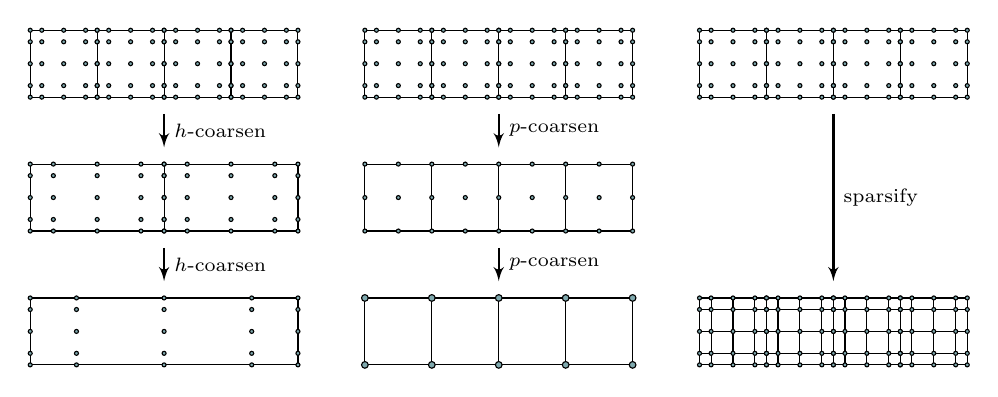
\begin{tikzpicture}[scale=0.85]
		% homg
		\draw (-5,4) grid +(4,1);
		\foreach \e in {-5,...,-2}
		\foreach \x in {0,0.1727,0.5,0.8273, 1.0} {
			\draw[fill=utsecblue] (\e+\x, 4) circle (0.03);
			\draw[fill=utsecblue] (\e+\x, 4.1727) circle (0.03);
			\draw[fill=utsecblue] (\e+\x, 4.5) circle (0.03);
			\draw[fill=utsecblue] (\e+\x, 4.8273) circle (0.03);
			\draw[fill=utsecblue] (\e+\x, 5) circle (0.03);
		}
		%\node at (5,4.5) {\small $p=4$};
		\draw[-latex',thick] (-3, 3.75) -- node[right] {{\scriptsize $h$-coarsen}} (-3, 3.25);
		\draw (-5,2) rectangle +(4,1);
		\draw (-3,2) -- (-3,3);
		\foreach \e in {-5,-3}
		\foreach \x in {0,0.1727,0.5,0.8273, 1.0} {
			\draw[fill=utsecblue] (\e+2*\x, 2) circle (0.03);
			\draw[fill=utsecblue] (\e+2*\x, 2.1727) circle (0.03);
			\draw[fill=utsecblue] (\e+2*\x, 2.5) circle (0.03);
			\draw[fill=utsecblue] (\e+2*\x, 2.8273) circle (0.03);
			\draw[fill=utsecblue] (\e+2*\x, 3) circle (0.03);
		}
		%\node at (5,2.5) {\small $p=2$};
	
		\draw[-latex',thick] (-3, 1.75) -- node[right] {{\scriptsize $h$-coarsen}} (-3, 1.25);
	
		\draw (-5,0) rectangle +(4,1);
		\foreach \x in {0,0.1727,0.5,0.8273, 1.0} {
			\draw[fill=utsecblue] (-5+4*\x, 0) circle (0.03);
			\draw[fill=utsecblue] (-5+4*\x, 0.1727) circle (0.03);
			\draw[fill=utsecblue] (-5+4*\x, 0.5) circle (0.03);
			\draw[fill=utsecblue] (-5+4*\x, 0.8273) circle (0.03);
			\draw[fill=utsecblue] (-5+4*\x, 1) circle (0.03);
		}
		
	%% p-multigrid
		\draw (0,4) grid +(4,1);
		\foreach \e in {0,...,3}
		\foreach \x in {0,0.1727,0.5,0.8273, 1.0} {
			\draw[fill=utsecblue] (\e+\x, 4) circle (0.03);
			\draw[fill=utsecblue] (\e+\x, 4.1727) circle (0.03);
			\draw[fill=utsecblue] (\e+\x, 4.5) circle (0.03);
			\draw[fill=utsecblue] (\e+\x, 4.8273) circle (0.03);
			\draw[fill=utsecblue] (\e+\x, 5) circle (0.03);
		}
		%\node at (5,4.5) {\small $p=4$};
	
		\draw[-latex',thick] (2, 3.75) -- node[right] {{\scriptsize $p$-coarsen}} (2, 3.25);
	
		\draw (0,2) grid +(4,1);
		\foreach \x in {0,0.5,...,4} {
			\draw[fill=utsecblue] (\x, 2) circle (0.03);
			\draw[fill=utsecblue] (\x, 2.5) circle (0.03);
			\draw[fill=utsecblue] (\x, 3) circle (0.03);
		}
		%\node at (5,2.5) {\small $p=2$};
	
		\draw[-latex',thick] (2, 1.75) -- node[right] {{\scriptsize $p$-coarsen}} (2, 1.25);
	
		\draw (0,0) grid +(4,1);
		\foreach \x in {0,1,2,3,4} {
			\draw[fill=utsecblue] (\x, 0) circle (0.05);
			\draw[fill=utsecblue] (\x, 1) circle (0.05);
		}
		%\node at (5,0.5) {\small $p=1$};
		
		%% collocated
			\draw (5,4) grid +(4,1);
			\foreach \e in {5,...,8}
			\foreach \x in {0,0.1727,0.5,0.8273, 1.0} {
				\draw[fill=utsecblue] (\e+\x, 4) circle (0.03);
				\draw[fill=utsecblue] (\e+\x, 4.1727) circle (0.03);
				\draw[fill=utsecblue] (\e+\x, 4.5) circle (0.03);
				\draw[fill=utsecblue] (\e+\x, 4.8273) circle (0.03);
				\draw[fill=utsecblue] (\e+\x, 5) circle (0.03);
			}
			%\node at (2, 1.8) {\tiny $p=4$};
	
			\draw[-latex',thick] (7, 3.75) -- node[right] {{\scriptsize sparsify}} (7, 1.25);
	
			\draw[step=0.5] (4.99,0) grid +(4.01,1);
			\draw (5,0.1727) -- (9,0.1727);
			\draw (5,0.8273) -- (9,0.8273);
			\foreach \e in {5,...,8} {
				\draw (\e+0.1727,0) -- (\e+0.1727,1);
				\draw (\e+0.8273,0) -- (\e+0.8273,1);
				\foreach \x in {0,0.1727,0.5,0.8273, 1.0} {
					\draw[fill=utsecblue] (\e+\x, 0) circle (0.03);
					\draw[fill=utsecblue] (\e+\x, 0.1727) circle (0.03);
					\draw[fill=utsecblue] (\e+\x, 0.5) circle (0.03);
					\draw[fill=utsecblue] (\e+\x, 0.8273) circle (0.03);
					\draw[fill=utsecblue] (\e+\x, 1) circle (0.03);
				}
			}
			% \node at (2, -0.2) {\tiny $p=1$ collocated with $p=4$};
		\end{tikzpicture}
		\caption{\label{fig:approaches} Different approaches
                  for high-order multigrid: high-order $h$-multigrid
                  (left), $p$-multigrid (middle) and low-order
                  multigrid based on the nodes of the nodes of the
                  high-order discretization, which can be used to
                  precondition the high-order system.}
\end{figure}

\subsubsection{$h$-multigrid}\label{subsec:h}
A direct approach to high-order multigrid is to use high-order
restriction and prolongation operators, and use the high-order
discretization of the operator for the residual computation on each
multigrid level (\S\ref{sub:restriction_&_prolongation}).
%A potential difficulty in this approach is that it
%requires smoothers for matrices arising from high-order
%discretization, which usually have less favorable properties compared
%to their low order counterparts; For instance, high-order
%discretizations of scalar elliptic operators are usually not
%M-matrices, which is a useful property to prove the convergence of
%smoothers such as Jacobi of Gauss-Seidel.
Due to the decreased sparsity of high-order discretized systems, the
efficient computation of the residual as well as devising efficient
smoothers can be a challenge. As a remedy, one can use matrix-free
methods which do not require to assemble system matrices but rely on
element-local computations. The performance of these element-local
computations can often be speed up using tensorized finite element
basis functions as common in spectral element methods; see
e.g.~\cite{DevilleFischerMund02}. 

\subsubsection{$p$-multigrid}\label{subsec:p}
In the $p$-multigrid approach to high-order multigrid, one (initially)
does not coarsen the mesh geometrically, but coarsens the finite
element system by
reducing the polynomial order. Starting from an order-$p$ polynomial
basis (for simplicity, we assume here that $p$ is a power of 2), the
coarser grids correspond to polynomials of order $p/2, p/4,\ldots,1$,
followed by geometric coarsening of the $p=1$ grid (i.e., the standard
low-order geometric multigrid). 
%Decreasing the polynomial order is an element-local operation and is particularly simple for discretizations with nonconforming meshes. \gsnote{Is that actually true?}. 
As for high-order $h$-multigrid, devising smoothers can be a challenge for
$p$-multigrid.  Moreover, one often finds dependence of the
convergence factor on the order of the polynomial basis
\cite{MadayMunoz89}.

\subsubsection{Preconditioning using AMG hierarchy of lower-order operator} \label{subsec:low}
In this defect correction approach (see
\cite{TrottenbergOosterleeSchuller01, Hackbusch85}), the high-order
defect/residual is iteratively corrected using a low order operator
obtained by overlaying the high-order nodes with a low order
(typically linear) finite element mesh. While the resulting low-order
operator has the same number of degrees of freedom as the high-order
operator, it is much sparser and can thus be assembled efficiently and
then provided as input to an algebraic multigrid method, which
computes a grid hierarchy through algebraic point aggregation.  This
construction of a low-order preconditioner based on the nodes of the
high-order discretization is used, for instance in~\cite{Brown10,
  Kim07, DevilleMund90, HeysManteuffelMcCormickEtAl05}.  Due to the
black-box nature of algebraic multigrid, it is particularly attractive
for high-order discretizations on unstructured meshes.  Even for
structured meshes, the solution of the low-order system with a
geometric multigrid method is not straightforward due to the non
evenly spaced node points inherited from the high-order
discretization.  In principle, this approach only requires computation
of the residual for the high-order discretized operator. Smoothing on
the finest level uses the low-order discretized operator, and either
the high-order or the low-order residual can be used in the
smoother. Using the high-order residual in the smoother requires an
additional high-order residual computation per smoothing step.


% The resulting method is nearly independent of $p$, but this low-order
% preconditioning is not work optimal and the convergence factors can be
% lower than when multigrid is applied directly to the high-order
% operator. \gsnote{Reference or remove statement.} 


% and the
%fact that the low-order system matrix is sparse and can thus be
%assembled efficiently.
%, where the construction of a
%grid hierarchy from geometric coarsening can be very difficult.
% For structured grids such as the ones used for
% the test problems in Section~\ref{sec:numerics}, a geometric multigrid
% method can be devised that either copes with the non evenly spaced
% points (which can be challenging) or replaces them by evenly spaced
% points---we experiment with the latter option in
% Section~\ref{sec:numerics}.

% multigrid cycles are faster compared to high
%order $h$-multigrid or $p$-multigrid discussed in
%Section~\ref{subsec:h} and Section~\ref{subsec:p}, respectively.

%Standard multigrid is then used for the low order operator, which has
%more favorable sparsity properties and thus allows for standard
%smoothers.
%  Thus, the speedup for a full multigrid cycle when using the
%low order operator is limited.

%The advantages of doing
%this are mainly in the simplicity of the approach and the availability
%of parallel multigrid solvers capable of solving such lower-order
%operators.
% The sparsity of the lower-order operators also permits the
%use of AMG for solving the lower-order operators, possibly obtained
%via discretizations on unstructured meshes.


% **********************************************************
\subsection{Smoothers}\label{subsec:smoothers}
Next, we summarize different smoothing approaches. In our numerical
comparisons, we restrict ourselves to the point smoothers reviewed in
\S\ref{subsec:ptsmoothers}. For completeness of the
presentation, we briefly describe Schwarz-type smoothers in
\S\ref{subsec:schwarz}.


\subsubsection{Point smoothers}\label{subsec:ptsmoothers}
In our numerical tests, we compare the Jacobi and the symmetric successive over
relaxation (SSOR) smoothers, as well as a Chebyshev-accelerated Jacobi
smoother~\cite{Brandt77}. All of these smoothers require the diagonal of the
system matrix; if matrices are not assembled (i.e., in a matrix-free approach),
these diagonal entries must be precomputed in a setup step.  Note that the
parallelization of Gauss-Seidel smoothers (such as SSOR) requires coloring of
unknowns at parallel boundaries, and, compared to Jacobi smoothing, more
complex communication in a distributed memory implementation. The
Chebyshev-accelerated Jacobi method is an attractive alternative to SSOR; it
can significantly improve over Jacobi smoothing, while being as simple to
implement~\cite{AdamsBrezinaHuEtAl03}. The acceleration of Jacobi smoothing
with Chebyshev polynomials requires estimation of the maximum eigenvalues of
the system matrix, which has to be done in a setup. For our experiments, we
estimated the largest eigenvalue using 10 iterations of the Arnoldi algorithm.

In Figures~\ref{fig:smoothers} and~\ref{fig:smoothers-var}, we compare the
efficiency of these point smoothers for different polynomial orders. In our
tests, we compute the eigenvectors of the system matrix, choose a zero right
hand side and an initialization that has all unit coefficients in the basis
given by these eigenvectors. For the polynomial orders $p=1,4,16$, we compare
the performance of point smoothers with and without a multigrid step.  We
depict the coefficients after 6 smoothing steps on the left, and the results
obtained for a two-grid method\footnote{For simplicity, we chose two grids in
our tests; the results for a multigrid v-cycle are very similar.} with 3 pre
and 3 post smoothing steps (and thus overall 6 smoothing steps on the finest
grid) on the left. The SSOR smoother uses a lexicographic ordering of the
unknowns, and we use 2 pre and 1 post smoothing steps, which again amounts to
overall 6 smoothing steps on the finest grid. The Chebyshev smoother targets
the part of the spectrum given by $[\lambda_\text{max}/4,\lambda_\text{max}]$,
where $\lambda_\text{max}$ is the maximum eigenvalue of the system matrix. 

The results for the constant coefficient Laplacian operator on the
unit square (Figure~\ref{fig:smoothers}) show that all point
smoothers decrease the error compoments in the upper half of the
spectrum, but that this damping factor is smaller for high-order
elements. Note that Chebyshev accelerated Jacobi smoothing results in
a uniform damping of a larger part of the spectrum than Jacobi
smoothing.  Both, the Chebyshev and SSOR methods outperform Jacobi
smoothing, in particular for higher orders. Combining the smoothers
with a two-grid cycle, all error components are decreased for all
smoothers (and thus the resulting two-grid methods converge, see
Table~\ref{tab:box} in the section summarizing our numerical tests),
but the error decreases slower for higher polynomial degrees. For high
polynomial order, a two-grid iteration with SSOR smoothing results in a
significantly better error reduction than Jacobi or Chebyshev
smoothing.

In Figure~\ref{fig:smoothers-var}, we study the solution of
\eqref{eq:Poisson} with a smoothly (but highly) varying coefficient
$\mu$ on a deformed geometry. Note that, comparing with the constant
coefficient case, now Jacobi smoothing performs significantly worse,
both, when used as a solver and as a smoother. In particular, for
$p=16$ Jacobi smoothing does not lead to a converging two-grid
algorithm (compare with Table~\ref{tab:2d-fan}). SSOR smoothing
combined with the two-grid method still retains a satisfactory
convergence rate. \todo{Hari, Chebyshev-based multigrid also seems to
  have values larger than 1 but seems to converge in the tables in the
  back...any idea why?}

\begin{figure}
	\centering
		\begin{tikzpicture}[scale=0.8]
		\begin{semilogyaxis}[ymajorgrids,ymin=1e-5,ymax=2,xmin=0,xmax=961]
		\addplot[color=black]  table[x=dof, y=u]{data/smoother-const-box.dat};
		\addplot[color=blue!70, opacity=0.5,only marks, mark=*,mark size=1pt]   table[x=dof, y=jacobi1]{data/smoother-const-box.dat};
		\addplot[color=red!70!black, opacity=0.5,only marks, mark=*,mark size=1pt] table[x=dof, y=chebyshev1]{data/smoother-const-box.dat};
		\addplot[color=green!70!black,only marks, opacity=0.5,mark=*,mark size=1pt]  table[x=dof, y=ssor1]{data/smoother-const-box.dat};
		\end{semilogyaxis}
		\draw[black, fill=white] (4.0, 3.7) rectangle +(2.85,2);
		% \draw[black] (4.0, 5.375) -- (6.85,5.375);
		\node at (5.35, 5.53) {\bf \small{smooth, $p=1$}}; 
		\node[fill=blue!70, draw, circle,minimum width=0.1cm] at (4.3, 5.0) {}; 
		\node[fill=red!70!black, draw, circle,minimum width=0.1cm] at (4.3, 4.5) {};
		\node[fill=green!70!black, draw, circle,minimum width=0.1cm] at (4.3, 4.0) {};
		\node[text width=1.9cm] at (5.75, 5.0) {\small jacobi $(6)$};
		\node[text width=1.9cm] at (5.75, 4.5) {\small chebyshev $(6)$};
		\node[text width=1.9cm] at (5.75, 4.0) {\small ssor $(3)$};
		\end{tikzpicture}
		\begin{tikzpicture}[scale=0.8]
		\begin{semilogyaxis}[ymajorgrids,ymin=1e-5,ymax=2,xmin=0,xmax=961,yticklabels={,,}]
		\addplot[color=black]  table[x=dof, y=u]{data/vcycle-const-box.dat};
		\addplot[color=blue!70,opacity=0.5,only marks, mark=*,mark size=1pt]   table[x=dof, y=jacobi1]{data/vcycle-const-box.dat};
		\addplot[color=red!70!black,opacity=0.5,only marks, mark=*,mark size=1pt] table[x=dof, y=chebyshev1]{data/vcycle-const-box.dat};
		\addplot[color=green!70!black,opacity=0.5,only marks, mark=*,mark size=1pt]  table[x=dof, y=ssor1]{data/vcycle-const-box.dat};
		\end{semilogyaxis}
		\draw[black, fill=white] (3.7, 3.7) rectangle +(3.15,2);
		%\draw[black] (4.0, 5.375) -- (6.85,5.375);
		\node at (5.35, 5.53) {\bf \small{v-cycle, $p=1$}}; 
		\node[fill=blue!70, draw, circle,minimum width=0.1cm] at (4.0, 5.0) {}; 
		\node[fill=red!70!black, draw, circle,minimum width=0.1cm] at (4.0, 4.5) {};
		\node[fill=green!70!black, draw, circle,minimum width=0.1cm] at (4.0, 4.0) {};
		\node[text width=2.1cm] at (5.55, 5.0) {\small jacobi $(3,3)$};
		\node[text width=2.1cm] at (5.55, 4.5) {\small chebyshev $(3,3)$};
		\node[text width=2.1cm] at (5.55, 4.0) {\small ssor $(2,1)$};
		\end{tikzpicture}
	\\
		\begin{tikzpicture}[scale=0.8]
		\begin{semilogyaxis}[ymajorgrids,ymin=1e-5,ymax=2,xmin=0,xmax=961]
		\addplot[color=black]  table[x=dof, y=u]{data/smoother-const-box.dat};
		\addplot[color=blue!70,opacity=0.5,only marks, mark=*,mark size=1pt]   table[x=dof, y=jacobi4]{data/smoother-const-box.dat};
		\addplot[color=red!70!black,opacity=0.5,only marks, mark=*,mark size=1pt] table[x=dof, y=chebyshev4]{data/smoother-const-box.dat};
		\addplot[color=green!70!black,opacity=0.5,only marks, mark=*,mark size=1pt]  table[x=dof, y=ssor4]{data/smoother-const-box.dat};
		\end{semilogyaxis}
		\draw[black, fill=white] (4.0, 5.375) rectangle +(2.85,0.325);
		\node at (5.35, 5.53) {\bf \small{smooth, $p=4$}};
		\end{tikzpicture}
		\begin{tikzpicture}[scale=0.8]
		\begin{semilogyaxis}[ymajorgrids,ymin=1e-5,ymax=2,xmin=0,xmax=961,yticklabels={,,}]
		\addplot[color=black]  table[x=dof, y=u]{data/vcycle-const-box.dat};
		\addplot[color=blue!70,only marks,opacity=0.5, mark=*,mark size=1pt]   table[x=dof, y=jacobi4]{data/vcycle-const-box.dat};
		\addplot[color=red!70!black,only marks,opacity=0.5, mark=*,mark size=1pt] table[x=dof, y=chebyshev4]{data/vcycle-const-box.dat};
		\addplot[color=green!70!black,only marks,opacity=0.5, mark=*,mark size=1pt]  table[x=dof, y=ssor4]{data/vcycle-const-box.dat};
		\end{semilogyaxis}
			\draw[black, fill=white] (4.0, 5.375) rectangle +(2.85,0.325);
			\node at (5.35, 5.53) {\bf \small{v-cycle, $p=4$}};
		\end{tikzpicture}
	\\
		\begin{tikzpicture}[scale=0.8]
		\begin{semilogyaxis}[ymajorgrids,ymin=1e-5,ymax=2,xmin=0,xmax=961]
		\addplot[color=black]  table[x=dof, y=u]{data/smoother-const-box.dat};
		\addplot[color=blue!70,opacity=0.5,only marks, mark=*,mark size=1pt]   table[x=dof, y=jacobi16]{data/smoother-const-box.dat};
		\addplot[color=red!70!black,opacity=0.5,only marks, mark=*,mark size=1pt] table[x=dof, y=chebyshev16]{data/smoother-const-box.dat};
		\addplot[color=green!70!black,opacity=0.5,only marks, mark=*,mark size=1pt]  table[x=dof, y=ssor16]{data/smoother-const-box.dat};
		\end{semilogyaxis}
		\draw[black, fill=white] (3.9, 5.375) rectangle +(2.95,0.325);
		\node at (5.35, 5.53) {\bf \small{smooth, $p=16$}};
		\end{tikzpicture}
		\begin{tikzpicture}[scale=0.8]
		\begin{semilogyaxis}[ymajorgrids,ymin=1e-5,ymax=2,xmin=0,xmax=961,yticklabels={,,}]
		\addplot[color=black]  table[x=dof, y=u]{data/vcycle-const-box.dat};
		\addplot[color=blue!70,opacity=0.5,only marks, mark=square*,mark size=1pt]   table[x=dof, y=jacobi16]{data/vcycle-const-box.dat};
		\addplot[color=red!70!black,opacity=0.4,only marks, mark=*,mark size=1pt] table[x=dof, y=chebyshev16]{data/vcycle-const-box.dat};
		\addplot[color=green!70!black,opacity=0.6,only marks, mark=diamond*,mark size=1pt]  table[x=dof, y=ssor16]{data/vcycle-const-box.dat};
		\end{semilogyaxis}
		\draw[black, fill=white] (3.95, 5.375) rectangle +(2.9,0.325);
		\node at (5.35, 5.53) {\bf \small{v-cycle, $p=16$}};
		\end{tikzpicture}
	\caption{\label{fig:smoothers} Error decay for different
          point smoothers when used as solver (left column) and when used
          within a single two-grid step (right column) for a two-dimensional,
          constant coefficient Laplace problem on a unit square. To
          keep the number of unknowns the same for
          different polynomial orders, meshes of $32\times 32$,
          $8\times 8$ and $2\times 2$ elements are used for polynomial
          orders $p=1$, $p=4$ and $p=16$, respectively.
          Plotted are the coefficients of the error
          expanded in the eigenvectors of the system matrix $A_k$.
          The order of the eigenvectors is such that the
          corresponding eigenvalues are descending; thus, the
          smoothness of the eigenvectors decays from left to right.
          The initialization is chosen to have all unit coefficients in
          the eigenvector expansion.}
\end{figure}

%% Variable Coefficients ----- SHELL

\begin{figure}
	\centering
		\begin{tikzpicture}[scale=0.8]
		\begin{semilogyaxis}[ymajorgrids,ymin=1e-5,ymax=2,xmin=0,xmax=961]
		\addplot[color=black]  table[x=dof, y=u]{data/smoother-var-shell.dat};
		\addplot[color=blue!70, opacity=0.5,only marks, mark=*,mark size=1pt]   table[x=dof, y=jacobi1]{data/smoother-var-shell.dat};
		\addplot[color=red!70!black, opacity=0.5,only marks, mark=*,mark size=1pt] table[x=dof, y=chebyshev1]{data/smoother-var-shell.dat};
		\addplot[color=green!70!black,only marks, opacity=0.5,mark=*,mark size=1pt]  table[x=dof, y=ssor1]{data/smoother-var-shell.dat};
		\end{semilogyaxis}
		\draw[black, fill=white] (4.0, 3.7) rectangle +(2.85,2);
		\node at (5.35, 5.53) {\bf \small{smooth, $p=1$}}; 
		\node[fill=blue!70, draw, circle,minimum width=0.1cm] at (4.3, 5.0) {}; 
		\node[fill=red!70!black, draw, circle,minimum width=0.1cm] at (4.3, 4.5) {};
		\node[fill=green!70!black, draw, circle,minimum width=0.1cm] at (4.3, 4.0) {};
		\node[text width=1.9cm] at (5.75, 5.0) {\small jacobi $(6)$};
		\node[text width=1.9cm] at (5.75, 4.5) {\small chebyshev $(6)$};
		\node[text width=1.9cm] at (5.75, 4.0) {\small ssor $(3)$};
		\end{tikzpicture}
		\begin{tikzpicture}[scale=0.8]
		\begin{semilogyaxis}[ymajorgrids,ymin=1e-5,ymax=2,xmin=0,xmax=961,yticklabels={,,}]
		\addplot[color=black]  table[x=dof, y=u]{data/vcycle-var-shell.dat};
		\addplot[color=blue!70,opacity=0.5,only marks, mark=*,mark size=1pt]   table[x=dof, y=jacobi1]{data/vcycle-var-shell.dat};
		\addplot[color=red!70!black,opacity=0.5,only marks, mark=*,mark size=1pt] table[x=dof, y=chebyshev1]{data/vcycle-var-shell.dat};
		\addplot[color=green!70!black,opacity=0.5,only marks, mark=*,mark size=1pt]  table[x=dof, y=ssor1]{data/vcycle-var-shell.dat};
		\end{semilogyaxis}
		\draw[black, fill=white] (3.7, 3.7) rectangle +(3.15,2);
		\node at (5.35, 5.53) {\bf \small{v-cycle, $p=1$}}; 
		\node[fill=blue!70, draw, circle,minimum width=0.1cm] at (4.0, 5.0) {}; 
		\node[fill=red!70!black, draw, circle,minimum width=0.1cm] at (4.0, 4.5) {};
		\node[fill=green!70!black, draw, circle,minimum width=0.1cm] at (4.0, 4.0) {};
		\node[text width=2.1cm] at (5.55, 5.0) {\small jacobi $(3,3)$};
		\node[text width=2.1cm] at (5.55, 4.5) {\small chebyshev $(3,3)$};
		\node[text width=2.1cm] at (5.55, 4.0) {\small ssor $(2,1)$};
		\end{tikzpicture}
	\\
		\begin{tikzpicture}[scale=0.8]
		\begin{semilogyaxis}[ymajorgrids,ymin=1e-5,ymax=2,xmin=0,xmax=961]
		\addplot[color=black]  table[x=dof, y=u]{data/smoother-var-shell.dat};
		\addplot[color=blue!70,opacity=0.5,only marks, mark=*,mark size=1pt]   table[x=dof, y=jacobi4]{data/smoother-var-shell.dat};
		\addplot[color=red!70!black,opacity=0.5,only marks, mark=*,mark size=1pt] table[x=dof, y=chebyshev4]{data/smoother-var-shell.dat};
		\addplot[color=green!70!black,opacity=0.5,only marks, mark=*,mark size=1pt]  table[x=dof, y=ssor4]{data/smoother-var-shell.dat};
		\end{semilogyaxis}
		\draw[black, fill=white] (4.0, 5.375) rectangle +(2.85,0.325);
		\node at (5.35, 5.53) {\bf \small{smooth, $p=4$}};
		\end{tikzpicture}
		\begin{tikzpicture}[scale=0.8]
		\begin{semilogyaxis}[ymajorgrids,ymin=1e-5,ymax=2,xmin=0,xmax=961,yticklabels={,,}]
		\addplot[color=black]  table[x=dof, y=u]{data/vcycle-var-shell.dat};
		\addplot[color=blue!70,only marks, mark=*,opacity=0.5,mark size=1pt]   table[x=dof, y=jacobi4]{data/vcycle-var-shell.dat};
		\addplot[color=red!70!black,only marks, mark=*,opacity=0.5,mark size=1pt] table[x=dof, y=chebyshev4]{data/vcycle-var-shell.dat};
		\addplot[color=green!70!black,only marks, mark=*,opacity=0.5,mark size=1pt]  table[x=dof, y=ssor4]{data/vcycle-var-shell.dat};
		\end{semilogyaxis}
		\draw[black, fill=white] (4.0, 5.375) rectangle +(2.85,0.325);
		\node at (5.35, 5.53) {\bf \small{v-cycle, $p=4$}};
		\end{tikzpicture}
	\\
		\begin{tikzpicture}[scale=0.8]
		\begin{semilogyaxis}[ymajorgrids,ymin=1e-5,ymax=2,xmin=0,xmax=961]
		\addplot[color=black]  table[x=dof, y=u]{data/smoother-var-shell.dat};
		\addplot[color=blue!70,opacity=0.5,only marks, mark=*,mark size=1pt]   table[x=dof, y=jacobi16]{data/smoother-var-shell.dat};
		\addplot[color=red!70!black,opacity=0.5,only marks, mark=*,mark size=1pt] table[x=dof, y=chebyshev16]{data/smoother-var-shell.dat};
		\addplot[color=green!70!black,opacity=0.5,only marks, mark=*,mark size=1pt]  table[x=dof, y=ssor16]{data/smoother-var-shell.dat};
		\end{semilogyaxis}
		\draw[black, fill=white] (3.9, 5.375) rectangle +(2.95,0.325);
		\node at (5.35, 5.53) {\bf \small{smooth, $p=16$}};
		\end{tikzpicture}
		\begin{tikzpicture}[scale=0.8]
		\begin{semilogyaxis}[ymajorgrids,ymin=1e-5,ymax=2,xmin=0,xmax=961,yticklabels={,,}]
		\addplot[color=black]  table[x=dof, y=u]{data/vcycle-var-shell.dat};
		\addplot[color=blue!70,opacity=0.5,only marks, mark=square*,mark size=1pt]   table[x=dof, y=jacobi16]{data/vcycle-var-shell.dat};
		\addplot[color=red!70!black,opacity=0.5,only marks, mark=*,mark size=1pt] table[x=dof, y=chebyshev16]{data/vcycle-var-shell.dat};
		\addplot[color=green!70!black,opacity=0.5,only marks, mark=diamond*,mark size=1pt]  table[x=dof, y=ssor16]{data/vcycle-var-shell.dat};
		\end{semilogyaxis}
		\draw[black, fill=white] (3.95, 5.375) rectangle +(2.9,0.325);
		\node at (5.35, 5.53) {\bf \small{v-cycle, $p=16$}};
		\end{tikzpicture}
	\caption{\label{fig:smoothers-var} Same as
          Figure~\ref{fig:smoothers}, but for the two-dimensional warped
          geometry shown in Figure~\ref{fig:mesh} with varying coefficient
          $\mu(x,y) = 1 + 10^6(\cos^2(2\pi x) + \cos^2(2\pi y))$.}
\end{figure}


\subsubsection{Schwarz-based smoothers}\label{subsec:schwarz}
An alternative smoothing approach for high-order discretizations is
based on local block solves.  Schwarz-type domain decomposition
smoothers have successfully been used for spectral element
discretizations with orders significantly higher than 8. They are more
stable for anisotropic meshes or anisotropic problems than point
smoothers. A main challenge of Schwarz-type smoothers is that they
require the solution of dense local systems.  This is either done by
using direct methods or approximations that allow for a fast iterative
solution \cite{LottesFischer05, FischerLottes05}. However, the
coarse-grid solves can become fairly expensive. Moreover, depending on
how much overlap between the domains is used, it is not
straightforward to achieve good parallel scalability.

\subsection{Comparing computational cost}\label{subsec:complexity}
To compare the computational cost of the different methods, we focus
on matrix-vector multiplications on the finest multigrid level, which
dominate the overall computation. Denoting the number of unknowns on
the finest level by $N$, the cost for a matrix-vector product is
$Ng_p$, where $g_p>0$ is the cost per unknown for the application of
an operator originating from a discretization with polynomial order
$p$. Since high-order discretizations result in less sparse operators,
we have $g_1\le g_2\le \ldots$. The actual value of $g_p$ depends
strongly on the implementation and on the system architecture.
% To
%illustrate this, consider an elemental matrix for a hexahedral mesh in
%three dimensions, which is dense and of size $(p+1)^3\times
%(p+1)^3$. Its naive application to a vector amounts to $\mathcal
%O((p+1)^6)$ operations; for tensor bases, as common in spectral
%element methods, this can be reduced to $\mathcal O((p+1)^4)$
%operations \cite{DevilleFischerMund02}.
In general, high-order implementations allow more memory locality,
which often results in higher performance compared to low order
methods.

The dominant computational cost per iteration of the high-order
multigrid approaches discussed in \S\ref{sec:approaches} can
thus be summarized as
\begin{equation}\label{eq:compcost}
  g_p(1+m(s_\text{pre}+s_\text{post})).
\end{equation}
Here, we denote by $s_\text{pre}$ and $s_\text{post}$ the number of
pre and post smoothing steps on the finest multigrid level,
respectively. Moreover, $m$ denotes the number of necessary residual
computations (and thus matrix-vector computations) per smoothing step.
Jacobi smoothing and Chebyshev-accelerated Jacobi require $m=1$
matrix-vector multiplication per smoothing step, while SSOR requires
$m=2$ matrix-vector operations. If, in the approach discussed in
\S\ref{subsec:low}, the linear-order residual is used in the
smoother, then the cost \eqref{eq:compcost} reduces to
\begin{equation}\label{eq:compcost2}
  g_p+g_1m(s_\text{pre}+s_\text{post})).
\end{equation}
However, since the overall number of iterations increases (see
\S\ref{subsec:results}), this usually does not decrease the
solution time.

% note that  Jacobi, SSOR and
%Chebyshev-accelerated Jacobi require a matrix-vector product, and we
%denote by $m$ the number of such products per smoothing step.


%\begin{itemize}
%\item {\em high-order $h$-multigrid:} On the finest grid level, the
%  residual and the smoothing steps are all based on the order $p$
%  discretization. Thus, the cost based on the matrix-vector products
%  on the finest multigrid level is
%  $g_p(1+m(s_\text{pre}+s_\text{post}))$.
%
%\item {\em $p$-multigrid:} As for high-order $h$-multigrid, an
%  estimate for the computational cost on the finest level is
%  $g_p(1+m(s_\text{pre}+s_\text{post}))$.
%
%\item {\em high-order defect correction with linear-order operator:}
%  high-order defect correction requires the computation of the
%  high-order residual, but uses smoothing based on the low-order
%  operator. Using linear elements, the computational cost on the
%  finest grid level is thus
%  $g_p(1+m(s_\text{pre}+s_\text{post}))$.
%\end{itemize}


If the overall number of unknowns $N$ is kept fixed and the problem
solution is smooth, it is well known that the accuracy increases for
high-order discretizations. Due to the decreased sparsity of the
discretized operators, this does not automatically translate into more
accuracy per computation time; see, e.g.~\cite{Brown10}. However, note
that the complexity of most computations in a multigrid preconditioned
conjugate gradient algorithm, for instance, are of complexity
$\mathcal{O}(N)$ (see Algorithm~\ref{alg:pcg}) and thus independent of
$g_p$. Thus, the computational cost of these steps does not depend on
the order of the discretization. Even if these $\mathcal{O}(N)$ steps
do not dominate the computation, they contribute to making high-order
discretizations favorable not only in terms of accuracy per unknown,
but also in terms of accuracy per computation time.

\begin{algorithm}[ht] 
  % v-cycle 
  \caption{Multigrid preconditioned Conjugate Gradient Method} \label{alg:pcg} 
  \begin{algorithmic}[1]
    \Require rhs and guess
    \Ensure  solution
    \While {not converged} 
    \State $\bs{h} = A \bs{p}$ 											\Comment $~~\quad\quad\quad\quad\mathcal{O}(Ng_p)$
    \State $\rho_r = (\rho, \bs{r})$								\Comment $~~\quad\quad\quad\quad\mathcal{O}(N)~~~$
    \State $\alpha = \rho_r / ( \bs{p}, \bs{h} )$		\Comment $~~\quad\quad\quad\quad\mathcal{O}(N)~~~$
    \State $\bs{u} = \bs{u} + \alpha\bs{p}$					\Comment $~~\quad\quad\quad\quad\mathcal{O}(N)~~~$
    \State $\bs{r} = \bs{r} - \alpha\bs{h}$					\Comment $~~\quad\quad\quad\quad\mathcal{O}(N)~~~$
    \State Convergence Test
    \State $\rho = M\bs{r}$ 												\Comment V-cycle $\quad\mathcal{O}(Ng_p)$
    \State $\beta = (\rho, \bs{r}) / \rho_r$				\Comment $~~\quad\quad\quad\quad\mathcal{O}(N)~~~$
    \State $\bs{p} = \rho + \beta\bs{p}$						\Comment $~~\quad\quad\quad\quad\mathcal{O}(N)~~~$
    \EndWhile
  \end{algorithmic}
\end{algorithm}




% **************************************************
% **************************************************
\section{Numerical results}\label{sec:numerics}
In this section we present a comprehensive comparison of our
algorithms for the solution of high-order discretizations of
\eqref{eq:Poisson}.  After introducing our test problems in
\S\ref{subsec:tests}, in \S\ref{subsec:measures} we
describe how we compare our methods for high-order multigrid. The
results for our test problem are then presented and discussed
\S\ref{subsec:results}.


\subsection{Presentation of test problems}\label{subsec:tests}
We compare our algorithms for the solution of~\eqref{eq:Poisson} on a
unit square and a unit cube with constant coefficient $\mu\equiv 1$,
as well as on the warped two and three dimensional domains shown in
Figure~\ref{fig:mesh}, where we use a varying coefficient $\mu(\bs
x)$. \todo{How anisotropic is the 2d-fan mesh? Probably we also have
  to update the mesh plots.}  We use isoparametric elements for these
deformed geometries, i.e., the geometry transformation is approximated
using the same polynomial order as the finite element functions. The
Jacobians for this transformation are computed at every quadrature
point. The coefficient $\mu$ at the coarse grid quadrature points is
computed as the linear interpolation of the coefficient at the fine
grid quadrature points. In our tests, change the polynomial degree of
the finite element functions but keep the same mesh; this results in
an increasing number of unknowns as $p$ increases.

\begin{figure}
	% 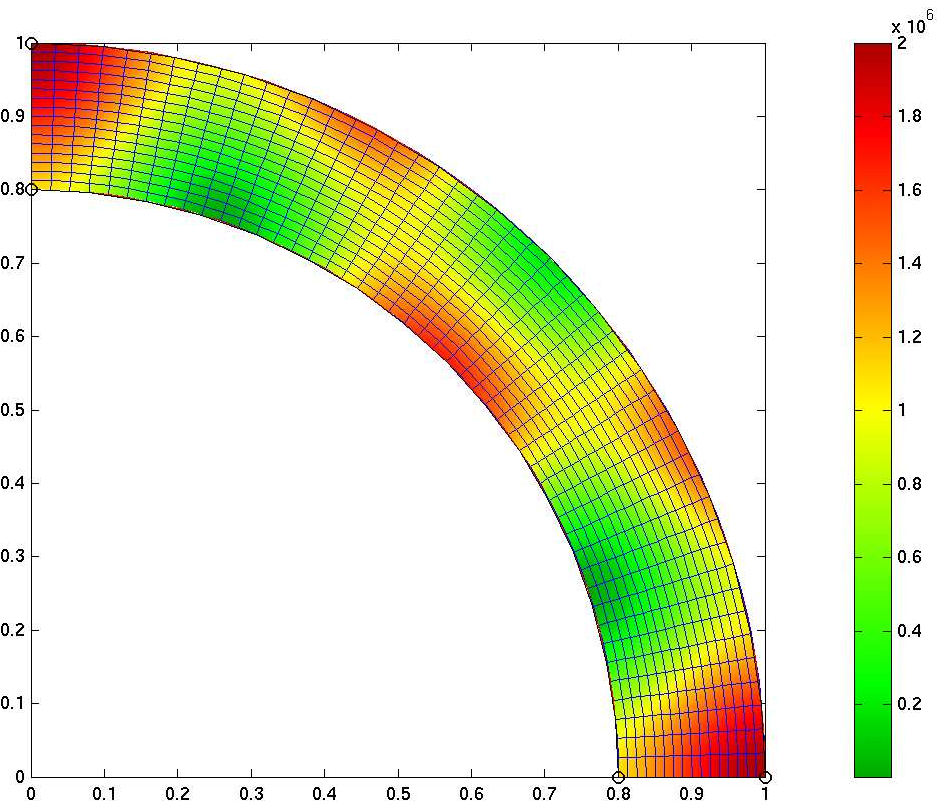
\includegraphics[width=0.48\textwidth]{figs/fan}
	% This file was created by matlab2tikz v0.3.3.
% Copyright (c) 2008--2013, Nico Schlömer <nico.schloemer@gmail.com>
% All rights reserved.
% 
% 
% 
\begin{tikzpicture}

\begin{axis}[%
width=1.8in,
height=2.0in,
view={0}{90},
scale only axis,
xmin=0,
xmax=0.8,
% xmajorgrids,
ymin=0.55,
ymax=1.05,
% ymajorgrids,
zmin=-1,
zmax=1,
% zmajorgrids,
axis x line*=bottom,
axis y line*=left,
axis z line*=left,
colormap/jet,
%colormap={traffic}{color(0cm)=(green); color(1cm)=(yellow); color(2cm)=(red)},
colorbar,
colorbar style={%title=$\mu$,
        width=0.15in, height=1.4in,
				at={(1.1,0.5)},anchor=east
    },
point meta min=3687.27158757943,
point meta max=2000001
]

\addplot3[%
surf,
colormap/jet,
%colormap={traffic}{color(0cm)=(green); color(1cm)=(yellow); color(2cm)=(red)},
shader=flat,
z buffer=sort,
point meta=explicit,
mesh/rows=65]
table[row sep=crcr,meta index=3,header=false] {
0 0.8 0 1095492.50281253\\
0.00981723062857594 0.799939761471316 0 1091470.11955702\\
0.0196329828183298 0.799759054956964 0 1079464.42475455\\
0.0294457783530871 0.79945790767068 0 1059658.73790523\\
0.0392541394619344 0.799036364964138 0 1032355.12786921\\
0.0490565890417669 0.79849449032012 0 997969.290417877\\
0.058851650879734 0.797832365342952 0 957023.521077331\\
0.0686378498755519 0.797050089746223 0 910137.92349953\\
0.0784137122636485 0.796147781337758 0 858020.028016915\\
0.0881777658351065 0.795125576001885 0 801453.025429382\\
0.097928540159373 0.793983627678968 0 741282.846764197\\
0.107664566805701 0.792722108342224 0 678404.340190066\\
0.117384379564289 0.791341207971825 0 613746.81104152\\
0.127086514667089 0.789841134526287 0 548259.199750399\\
0.136769511008241 0.788222113911153 0 482895.175268579\\
0.146431910364113 0.786484389944973 0 418598.418333033\\
0.156072257612903 0.784628224322584 0 356288.359850942\\
0.165689100953775 0.782653896575702 0 296846.625089343\\
0.175280992125496 0.780561704030823 0 241104.414690027\\
0.184846486624537 0.778351961764448 0 189831.029359803\\
0.194384143922611 0.776025002555635 0 143723.717069281\\
0.203892527683612 0.773581176835882 0 103398.990467864\\
0.213370205979919 0.771020852636352 0 69385.5287825629\\
0.222815751508043 0.768344415532453 0 42118.74354135\\
0.23222774180357 0.765552268585767 0 21937.051887418\\
0.241604759455383 0.762644832283355 0 9079.86585794335\\
0.250945392319113 0.759622544474429 0 3687.27158757943\\
0.26024823372981 0.756485860304417 0 5801.33971023018\\
0.269511882713776 0.753235252146417 0 15368.9779524042\\
0.278734944199548 0.74987120953006 0 32246.2096351285\\
0.287916029227991 0.746394239067791 0 56203.7380324736\\
0.29705375516147 0.742804864378573 0 86933.6366739991\\
0.306146745892072 0.739103626009029 0 124056.990018216\\
0.315193632048839 0.735291081352046 0 167132.297646148\\
0.324193051203992 0.731367804562825 0 215664.448299602\\
0.33314364807811 0.727334386472418 0 269114.067682562\\
0.342044074744226 0.723191434498755 0 326907.045820135\\
0.350892990830822 0.718939572555163 0 388444.055699444\\
0.359689063723685 0.714579440956412 0 453109.884590414\\
0.368430968766592 0.710111696322283 0 520282.412480874\\
0.377117389460798 0.705537011478684 0 589341.08802169\\
0.385747017663298 0.700856075356325 0 659674.770781799\\
0.394318553783827 0.696069592886969 0 730688.828947614\\
0.402830706980574 0.69117828489727 0 801811.403337476\\
0.411282195354577 0.686182888000218 0 872498.771206958\\
0.419671746142775 0.681084154484212 0 942239.766270842\\
0.427998095909678 0.675882852199766 0 1010559.23415821\\
0.436259990737637 0.670579764443871 0 1077020.52467328\\
0.444456186415682 0.665175689842036 0 1141227.0433196\\
0.452585448626891 0.65967144222802 0 1202822.9041664\\
0.460646553134276 0.654067850521267 0 1261492.74395132\\
0.468638285965151 0.648365758602076 0 1316960.77303442\\
0.476559443593947 0.642566025184516 0 1368989.15221189\\
0.48440883312346 0.636669523687107 0 1417375.79528847\\
0.492185272464501 0.630677142101285 0 1461951.70557531\\
0.499887590513909 0.624589782857676 0 1502577.9600611\\
0.507514627330917 0.61840836269019 0 1539142.45788661\\
0.515065234311833 0.612133812497967 0 1571556.54997335\\
0.522538274363021 0.605767077205188 0 1599751.66430049\\
0.529932622072137 0.599309115618768 0 1623676.03651431\\
0.537247163877615 0.592760900283967 0 1643291.64845463\\
0.544480798236363 0.58612341733793 0 1658571.46798795\\
0.551632435789654 0.579397666361174 0 1669497.07247182\\
0.558700999527178 0.572584660227055 0 1676056.72548753\\
0.565685424949238 0.565685424949238 0 1678243.96243677\\
0 0.802794162649704 0 1106059.01339602\\
0.00985151930250831 0.802733713725711 0 1101998.64441145\\
0.0197015550024464 0.802552376057117 0 1089879.79324566\\
0.0295486237206691 0.802250176952709 0 1069888.16138141\\
0.0393912425248479 0.80182716192256 0 1042329.71989186\\
0.0492279291527948 0.801283394671178 0 1007625.48722326\\
0.0590572022356859 0.80061895708791 0 966304.366046764\\
0.0688775815211497 0.799833949234612 0 918994.182975112\\
0.0786875880961881 0.798928489330581 0 866411.11020658\\
0.0884857446098949 0.797902713734746 0 809347.679275017\\
0.0982705754959396 0.796756776925139 0 748659.623359631\\
0.108040607194782 0.795490851475629 0 685251.805475526\\
0.117794368375586 0.794105128029933 0 620063.504901325\\
0.127530390157794 0.792599815272903 0 554053.343129032\\
0.137247206332338 0.790975139899104 0 488184.133324373\\
0.146943353582443 0.789231346578672 0 423407.933800245\\
0.156617371703999 0.787368697920466 0 360651.576520972\\
0.16626780382546 0.785387474432523 0 300802.926504708\\
0.175893196627246 0.783287974479813 0 244698.107642326\\
0.185492100560606 0.781070514239306 0 193109.905487777\\
0.195063070065915 0.778735427652357 0 146737.528681051\\
0.204604663790371 0.776283066374418 0 106197.878603358\\
0.214115444805055 0.773713799722076 0 72018.4424551889\\
0.223593980821329 0.771028014617439 0 44631.8890454495\\
0.233038844406536 0.768226115529865 0 24372.4100494098\\
0.242448613198959 0.76530852441505 0 11473.8131881888\\
0.25182187012203 0.762275680651484 0 6069.3385234226\\
0.261157203597734 0.759128040974282 0 8193.13561509826\\
0.270453207759189 0.755866079406401 0 17783.3083549916\\
0.27970848266236 0.752490287187256 0 34686.4064740009\\
0.28892163449689 0.749001172698738 0 58663.2185423479\\
0.298091275796003 0.745399261388654 0 89395.7011441975\\
0.307216025645447 0.741685095691598 0 126494.863107523\\
0.316294509891458 0.737859234947264 0 169509.412386431\\
0.325325361347702 0.733922255316206 0 217934.966493356\\
0.334307220001167 0.729874749693076 0 271223.625219318\\
0.343238733216979 0.725717327617332 0 328793.706615202\\
0.3521185559421 0.721450615181448 0 390039.453594435\\
0.36094535090789 0.71707525493662 0 454340.528732386\\
0.369717788831494 0.71259190579601 0 521071.128483408\\
0.37843454861603 0.708001242935506 0 589608.564657724\\
0.387094317549535 0.703303957692049 0 659341.180097982\\
0.395695791502662 0.698500757459518 0 729675.486539867\\
0.404237675125073 0.693592365582202 0 800042.435087385\\
0.412718682040512 0.688579521245863 0 869902.753033067\\
0.421137535040535 0.683462979366418 0 938751.304368454\\
0.429492966276847 0.678243510476256 0 1006120.45474383\\
0.437783717452236 0.672921900608191 0 1071582.44436269\\
0.446008540010072 0.667498951177096 0 1134750.79389021\\
0.454166195322331 0.661975478859207 0 1195280.78851669\\
0.46225545487613 0.65635231546914 0 1252869.10349947\\
0.470275100458732 0.650630307834617 0 1307252.6505189\\
0.478223924341014 0.64481031766894 0 1358206.73779087\\
0.486100729459336 0.638893221441221 0 1405542.64790557\\
0.49390432959582 0.632879910244387 0 1449104.74569174\\
0.50163354955699 0.626771289660985 0 1488767.23397542\\
0.509287225350749 0.620568279626806 0 1524430.67790573\\
0.516864204361677 0.614271814292345 0 1556018.41859838\\
0.524363345524604 0.607882841882121 0 1583472.99429014\\
0.531783519496454 0.601402324551879 0 1606752.68213478\\
0.539123608826322 0.59483123824369 0 1625828.26637138\\
0.546382508123754 0.588170572538983 0 1640680.12906118\\
0.553559124225214 0.581421330509514 0 1651295.748149\\
0.560652376358717 0.574584528566305 0 1657667.67451414\\
0.567661196306582 0.567661196306582 0 1659792.04520717\\
0 0.805598084480548 0 1117150.5969834\\
0.00988592773660569 0.805537424426398 0 1113052.23317079\\
0.0197703666888575 0.805355453399129 0 1100820.20750763\\
0.0296518282966072 0.805052198802908 0 1080642.63052473\\
0.0395288244480833 0.804627706306763 0 1052829.41922026\\
0.0493998677039961 0.8040820398377 0 1017806.97302782\\
0.0592634715215396 0.803415281571084 0 976110.871908486\\
0.0691181504782601 0.802627531918258 0 928376.744016492\\
0.0789624204957551 0.80171890951142 0 875329.48652106\\
0.0887947990631701 0.800689551185764 0 817771.055025297\\
0.0986138054604592 0.799539611958867 0 756567.063893577\\
0.108417960981376 0.798269265007347 0 692632.4611017\\
0.118205789156161 0.796878701640782 0 626916.556523361\\
0.127975815973895 0.7953681312729 0 560387.691582039\\
0.137726570104475 0.793737781390042 0 494017.840809911\\
0.147456583120196 0.791987897516904 0 428767.432106166\\
0.157164389716886 0.79011874317956 0 365570.662575316\\
0.166848527934582 0.788130599865779 0 305321.571099596\\
0.176507539377687 0.78602376698263 0 248861.107743159\\
0.186139969434608 0.783798561811396 0 196965.414305252\\
0.195744367496808 0.781455319459791 0 150335.500542782\\
0.205319287177268 0.778994392811493 0 109588.467558516\\
0.214863286528303 0.776416152473005 0 75250.3944466329\\
0.224374928258716 0.773720986717838 0 47750.967383899\\
0.233852779950249 0.77090930142804 0 27419.8928442179\\
0.2432954142733 0.767981520033075 0 14485.0993756032\\
0.252701409201872 0.764938083446051 0 9072.69625545298\\
0.262069348227727 0.761779449997323 0 11208.6231203139\\
0.271397820573705 0.75850609536547 0 20821.8930644021\\
0.280685421406185 0.75511851250566 0 37749.3033420358\\
0.289930752046643 0.751617211575412 0 61741.4632164648\\
0.299132420182293 0.748002719857764 0 92469.9680845844\\
0.308289040075758 0.744275581681877 0 129535.533070765\\
0.317399232773764 0.74043635834105 0 172476.888002443\\
0.3264616263148 0.736485628008195 0 220780.229116779\\
0.335474855935734 0.732423985648769 0 273889.020950046\\
0.344437564277337 0.728252042931171 0 331213.944471686\\
0.353348401588701 0.72397042813463 0 392142.794388316\\
0.362206025930503 0.719579786054584 0 456050.139318726\\
0.371009103377099 0.71508077790558 0 522306.572815655\\
0.379756308217405 0.710474081221698 0 590287.400511161\\
0.388446323154547 0.705760389754513 0 659380.628472728\\
0.397077839504239 0.700940413368622 0 728994.139629903\\
0.405649557391869 0.696014877934739 0 798561.968303927\\
0.414160185948253 0.690984525220383 0 867549.606881821\\
0.422608443504033 0.685850112778169 0 935458.302969024\\
0.430993057782698 0.680612413831726 0 1001828.32940163\\
0.439312766092178 0.675272217159249 0 1066241.23280404\\
0.447566315515003 0.669830326974715 0 1128321.08848591\\
0.455752463096991 0.664287562806767 0 1187734.80997771\\
0.463869976034425 0.658644759375303 0 1244191.58005514\\
0.471917631859717 0.652902766465763 0 1297441.48640473\\
0.479894218625499 0.647062448801157 0 1347273.45890097\\
0.487798535087147 0.641124685911846 0 1393512.61662509\\
0.495629390883674 0.635090372003077 0 1436017.14114092\\
0.503385606717002 0.628960415820331 0 1474674.79809628\\
0.511066014529557 0.622735740512461 0 1509399.2319356\\
0.518669457680172 0.616417283492672 0 1540126.15843819\\
0.526194791118277 0.61000599629735 0 1566809.57703065\\
0.533640881556335 0.603502844442763 0 1589418.11949898\\
0.541006607640517 0.596908807279662 0 1607931.64401974\\
0.548290860119567 0.590224877845787 0 1622338.17354753\\
0.555492542011855 0.583452062716327 0 1632631.26577499\\
0.562610568770578 0.576591381852326 0 1638807.88838059\\
0.569643868447089 0.569643868447089 0 1640866.8583786\\
0 0.808411799578459 0 1128758.6612471\\
0.0099204563491548 0.808350927656737 0 1124622.31046893\\
0.0198394187140737 0.808168321058658 0 1112277.14320249\\
0.0297553933355094 0.807864007284104 0 1091913.70651377\\
0.0396668869041577 0.807438032161611 0 1063845.90770985\\
0.0495724067855446 0.806890459841465 0 1028505.58640094\\
0.0594704612448111 0.806221372786043 0 986435.07100406\\
0.0693595596713638 0.805430871757395 0 938277.870887016\\
0.0792382128033544 0.804519075802067 0 884767.692372994\\
0.0891049329519579 0.803486122233178 0 826715.99944329\\
0.0989582342254126 0.802332166609734 0 764998.367456264\\
0.10879663275279 0.801057382713209 0 700539.899947234\\
0.11861864690746 0.799661962521368 0 634299.994140844\\
0.12842279753022 0.798146116179359 0 567256.749908305\\
0.138207608152047 0.796510071968065 0 500391.319417019\\
0.147971605216455 0.794754076269728 0 434672.490695912\\
0.157713318301399 0.792878393530839 0 371041.787985318\\
0.167431280340723 0.790883306222321 0 310399.355417933\\
0.177124027845087 0.788769114796982 0 253590.86879083\\
0.186790101122372 0.786536137644277 0 201395.693565653\\
0.196428044497495 0.784184711042349 0 154516.476507713\\
0.206036406531637 0.781715189107396 0 113570.32436044\\
0.215613740240816 0.779127943740339 0 79081.6865244692\\
0.225158603313804 0.776423364570812 0 51477.0207798929\\
0.234669558329332 0.77360185889849 0 31081.2825753586\\
0.244145172972558 0.770663851631749 0 18116.2402134318\\
0.253584020250771 0.767609785223677 0 12700.5812556264\\
0.262984678708289 0.764440119605441 0 14851.7404617046\\
0.272345732640528 0.761155332117023 0 24489.347298349\\
0.281665772307197 0.757755917435339 0 41440.1621412546\\
0.290943394144605 0.754242387499734 0 65444.3452859129\\
0.300177200977029 0.750615271434894 0 96162.8821952112\\
0.309365802227124 0.746875115471155 0 133185.972345622\\
0.31850781412534 0.743022482862248 0 176042.177765299\\
0.327601859918313 0.739057953800474 0 224208.120942899\\
0.336646570076197 0.734982125329327 0 277118.520165059\\
0.34564058249891 0.730795611253582 0 334176.353343672\\
0.354582542721266 0.726499042046859 0 394762.948752293\\
0.363471104116944 0.722093064756678 0 458247.812447794\\
0.372304928101295 0.717578342907011 0 523998.0170776\\
0.381082684332918 0.712955556398363 0 591386.994773971\\
0.389803050914013 0.708225401405379 0 659802.597379409\\
0.398464714589449 0.703388590272 0 728654.309766252\\
0.407066370944536 0.698445851404193 0 797379.525929546\\
0.415606724601466 0.69339792916025 0 865448.822265202\\
0.424084489414394 0.688245583738694 0 932370.187428312\\
0.432498388663121 0.682989591063793 0 997692.192856882\\
0.440847155245369 0.67763074266871 0 1061006.11193697\\
0.4491295318676 0.672169845576304 0 1121947.01841283\\
0.457344271234361 0.666607722177589 0 1180193.91559771\\
0.465490136236118 0.66094521010789 0 1235468.966861\\
0.473565900135565 0.655183162120696 0 1287535.91445788\\
0.481570346752364 0.64932244595924 0 1336197.78779432\\
0.489502270646297 0.643363944225818 0 1381294.01350695\\
0.497360477298802 0.637308554248874 0 1422697.04817384\\
0.505143783292861 0.631157187947865 0 1460308.66000088\\
0.512851016491221 0.624910771695931 0 1494055.98845272\\
0.520481016212912 0.618570246180381 0 1523887.51056866\\
0.528032633408041 0.612136566261036 0 1549769.0397221\\
0.535504730830835 0.605610700826428 0 1571679.87699165\\
0.542896183210907 0.598993632647887 0 1589609.22729121\\
0.550205877422717 0.59228635823154 0 1603552.98217132\\
0.557432712653203 0.585489887668245 0 1613510.95899488\\
0.564575600567562 0.578605244481467 0 1619484.67227417\\
0.571633465473148 0.571633465473149 0 1621475.69761759\\
0 0.811235342148411 0 1140873.76503478\\
0.00995510555990333 0.811174257619126 0 1136699.45225934\\
0.0199087119175271 0.810991013230378 0 1124241.2277503\\
0.0298593200963661 0.810685636578096 0 1103692.10303387\\
0.0398054315714298 0.810258173650881 0 1075370.02080811\\
0.0497455484949147 0.809708688823079 0 1039712.32096137\\
0.0596781739217748 0.809037264845083 0 997268.1525968\\
0.0696018120351558 0.808244002830873 0 948688.987108779\\
0.0795149683716599 0.807329022242793 0 894717.425289153\\
0.0894161500464063 0.806292460873552 0 836174.524836355\\
0.0993038659778542 0.80513447482548 0 773945.902744176\\
0.109176627112354 0.803855238487017 0 708966.889246603\\
0.119032946648394 0.80245494450645 0 642207.025832962\\
0.128871340260506 0.800933803762902 0 574654.209031998\\
0.138690326322802 0.799292045334573 0 507298.784074385\\
0.148488426132096 0.797529916464243 0 441117.888232126\\
0.158264164130598 0.79564768252204 0 377060.332819672\\
0.168016068128123 0.793645626965471 0 316032.295903292\\
0.177742669523799 0.791524051296739 0 258884.075224976\\
0.187442503527235 0.789283275017336 0 206398.123356055\\
0.197114109379107 0.786923635579928 0 159278.555412247\\
0.206756030571149 0.784445488337534 0 118142.284629374\\
0.216366815065495 0.781849206490013 0 83511.9036212271\\
0.225945015513353 0.779135181027863 0 55810.3901563053\\
0.235489189472965 0.776303820673334 0 35357.6767460209\\
0.24499789962684 0.773355551818882 0 22369.0841649384\\
0.254469713998204 0.77029081846295 0 16955.5811157208\\
0.263903206166653 0.767110082143111 0 19125.7964382811\\
0.273296955482966 0.763813821866554 0 28789.6772943715\\
0.282649547283048 0.760402534037951 0 45763.6572889673\\
0.291959573100976 0.756876732384703 0 69777.1730624125\\
0.301225630881107 0.753236947879569 0 100480.346927779\\
0.310446325189222 0.749483728660708 0 137452.636937324\\
0.319620267422675 0.745617639949128 0 180212.244515251\\
0.32874607601951 0.741639263963569 0 228226.063541276\\
0.337822376666519 0.737549199832821 0 280919.953441199\\
0.346847802506211 0.733348063505497 0 337689.12225474\\
0.355820994342652 0.729036487657275 0 397908.413523794\\
0.364740600846157 0.724615121595619 0 460942.302802458\\
0.373605278756796 0.720084631161995 0 526154.425185028\\
0.382413693086683 0.715445698631597 0 592916.473970096\\
0.391164517321019 0.710699022610601 0 660616.331873662\\
0.399856433617862 0.705845317930957 0 728665.319488201\\
0.40848813300659 0.700885315542735 0 796504.470360817\\
0.417058315585025 0.695819762404052 0 863609.767535379\\
0.425565690715194 0.690649421368576 0 929496.302089035\\
0.434008977217695 0.685375071070651 0 993721.339537437\\
0.442386903564637 0.67999750580803 0 1055886.30446709\\
0.45069820807113 0.674517535422262 0 1115637.71690545\\
0.458941639085285 0.66893598517673 0 1172667.13534045\\
0.467115955176714 0.66325369563237 0 1226710.18059054\\
0.47521992532348 0.657471522521086 0 1277544.7316038\\
0.48325232909749 0.651590336616882 0 1324988.39849537\\
0.491211956848279 0.64561102360472 0 1368895.38954266\\
0.499097609885186 0.639534483947148 0 1409152.8973376\\
0.50690810065787 0.633361632748685 0 1445677.13479356\\
0.514642252935149 0.627093399618018 0 1478409.15422801\\
0.522298901982139 0.620730728528 0 1507310.58234802\\
0.529876894735658 0.614274577673492 0 1532359.40076071\\
0.537375089977869 0.607725919327066 0 1553545.89576438\\
0.54479235850815 0.601085739692581 0 1570868.89283456\\
0.552127583313144 0.594355038756665 0 1584332.38062327\\
0.559379659734976 0.587534830138122 0 1593942.61668724\\
0.566547495637612 0.580626140935283 0 1599705.7928235\\
0.573630011571331 0.573630011571331 0 1601626.32210926\\
0 0.814068746514849 0 1153485.61186419\\
0.009989875790065 0.814007448635427 0 1149273.37928466\\
0.0199782471415817 0.813823564228395 0 1136702.23372315\\
0.0299636098425646 0.813517120986068 0 1115967.67954572\\
0.03994446013412 0.813088165057672 0 1087391.74064882\\
0.0499192949369066 0.812536761042391 0 1051417.31824921\\
0.0598866120774932 0.811862991979643 0 1008600.45547526\\
0.0698449105145812 0.811066959336569 0 959600.667752833\\
0.0797926905650555 0.810148782992758 0 905169.53684466\\
0.0897284541298312 0.80910860122219 0 846137.800593815\\
0.0996507049194623 0.807946570672413 0 783401.199162967\\
0.109557948679477 0.806662866340954 0 717905.361222627\\
0.119448693415405 0.805257681548963 0 650630.029654014\\
0.129321449617473 0.803731227912101 0 582572.93559821\\
0.13917473048491 0.802083735308671 0 514733.631982628\\
0.14900705214986 0.800315451845 0 448097.593045557\\
0.158816933900848 0.798426643818073 0 383620.875089978\\
0.168602898405765 0.79641759567543 0 322215.616122493\\
0.178363471934352 0.794288609972334 0 264736.628715114\\
0.188097184580138 0.792040007326198 0 211969.312041691\\
0.197802570481803 0.789672126368311 0 164619.076371916\\
0.207478168043927 0.787185323692835 0 123302.437226392\\
0.217122520157109 0.784579973803107 0 88539.89783927\\
0.226734174417395 0.781856469055235 0 60750.6985088291\\
0.236311683345008 0.779015219599018 0 40249.4708175443\\
0.245853604602331 0.776056653316173 0 27244.7945307393\\
0.255358501211122 0.772981215755899 0 21839.6161538663\\
0.264824941768913 0.76978937006778 0 24033.451495488\\
0.274251500664576 0.766481596932037 0 33726.2609148067\\
0.283636758293015 0.763058394487137 0 50723.8558971596\\
0.292979301268954 0.759520278254777 0 74744.6697526212\\
0.302277722639784 0.755867781062246 0 105427.704003156\\
0.311530622097449 0.752101452962188 0 142341.445715321\\
0.320736606189326 0.748221861149761 0 184993.539820795\\
0.329894288528073 0.74422958987722 0 232840.994389724\\
0.339002290000414 0.740125240365935 0 285300.695802508\\
0.348059238974829 0.735909430715846 0 341760.014609372\\
0.357063771508117 0.731582795812379 0 401587.291274762\\
0.3660145315508 0.727145987230835 0 464142.003584625\\
0.374910171151339 0.722599673138268 0 528784.433781532\\
0.38374935065913 0.717944538192856 0 594884.672956555\\
0.392530738926253 0.713181283440801 0 661830.822294058\\
0.401253013507936 0.708310626210746 0 729036.274833579\\
0.409914860861708 0.703333300005754 0 795945.986866308\\
0.41851497654522 0.698250054392845 0 862041.674309212\\
0.427052065412684 0.693061654890111 0 926845.895800439\\
0.435524841809917 0.687768882851431 0 989925.010266944\\
0.44393202976796 0.682372535348806 0 1050891.02179999\\
0.45227236319523 0.676873425052321 0 1109402.34835554\\
0.460544586068192 0.671272380107759 0 1165163.5726489\\
0.468747452620508 0.665570244011887 0 1217924.25327121\\
0.476879727530647 0.659767875485426 0 1267476.89121792\\
0.484940186107923 0.653866148343735 0 1313654.16145013\\
0.49292761447692 0.647865951365212 0 1356325.53063715\\
0.500840809760308 0.641768188157451 0 1395393.39074616\\
0.508678580259983 0.635573777021162 0 1430788.84360463\\
0.516439745636537 0.629283650811879 0 1462467.27397632\\
0.524123137087014 0.62289875679947 0 1490403.84812383\\
0.531727597520922 0.616420056525489 0 1514589.07139483\\
0.53925198173449 0.609848525658366 0 1535024.53221903\\
0.546695156583135 0.603185153846479 0 1551718.9512332\\
0.5540560011521 0.596430944569111 0 1564684.64328834\\
0.56133340692527 0.589586914985337 0 1573934.48709102\\
0.568526277952104 0.582654095780837 0 1579479.48246715\\
0.575633531012682 0.575633531012683 0 1581326.95900692\\
0 0.816912047122103 0 1166583.04461129\\
0.0100247674623247 0.816850535147374 0 1162332.9517384\\
0.0200480252315436 0.816666008486664 0 1149649.07342786\\
0.0300682638419051 0.81635849492901 0 1128729.43573705\\
0.0400839742823317 0.815928040784822 0 1099900.19032139\\
0.0500936482236719 0.815374710878911 0 1063609.8617628\\
0.0600957782458484 0.814698588540726 0 1020421.46170892\\
0.0700888580648708 0.813899775591803 0 971002.632866775\\
0.0800713827596758 0.812978392330435 0 916114.025717457\\
0.0900418489987628 0.811934577513551 0 856596.145825447\\
0.0999987552665905 0.810768488335824 0 793354.939009486\\
0.109940602089699 0.809480300405995 0 727346.404774053\\
0.119865892262527 0.808070207720426 0 659560.544791291\\
0.129773131072881 0.806538422633891 0 591004.96256875\\
0.139660826527039 0.804885175827589 0 522688.432618597\\
0.149527489574435 0.803110716274408 0 455604.752521702\\
0.159371634331906 0.801215311201429 0 390717.179496963\\
0.169191778307461 0.799199246049684 0 328943.734852257\\
0.17898644262354 0.797062824431171 0 271143.635572495\\
0.188754152239724 0.794806368083125 0 218105.082991974\\
0.198493436174872 0.792430216819574 0 170534.60481507\\
0.208202827728649 0.789934728480157 0 129048.109593184\\
0.2178808647024 0.787320278876239 0 94163.7731004306\\
0.227526089619356 0.784587261734314 0 66296.8348749769\\
0.237137049944122 0.781736088636711 0 45756.3415135087\\
0.246712298301425 0.778767188959611 0 32743.8321103512\\
0.256250392694082 0.775681009808383 0 27353.9214629918\\
0.265749896720164 0.772478015950258 0 29576.6991974342\\
0.275209379789304 0.769158689744328 0 39301.8285874587\\
0.284627417338147 0.765723531068911 0 56324.198234249\\
0.294002591044881 0.762173057246267 0 80350.9535017492\\
0.303333489042831 0.758507802964695 0 111009.713105757\\
0.312618706133078 0.754728320198007 0 147857.75983531\\
0.321856843996084 0.750835178122406 0 190391.983212912\\
0.331046511402267 0.746828963030769 0 238059.346012495\\
0.340186324421518 0.742710278244352 0 290267.64586069\\
0.349274906631614 0.738479744021935 0 346396.347439662\\
0.358310889325505 0.73413799746641 0 405807.269773256\\
0.367292911717435 0.729685692428838 0 467854.926303852\\
0.37621962114787 0.725123499409982 0 531896.332468335\\
0.385089673287205 0.720452105459328 0 597300.115709242\\
0.393901732338214 0.715672214071623 0 663454.785717575\\
0.402654471237217 0.710784545080928 0 729776.047574827\\
0.411346571853931 0.705789834552215 0 795713.06670958\\
0.419976725189975 0.700688834670518 0 860753.621578138\\
0.428543631576002 0.695482313627655 0 924428.107106821\\
0.437046000867421 0.690171055506545 0 986312.378613807\\
0.445482552638691 0.684755860163125 0 1046029.45162078\\
0.453852016376147 0.679237543105893 0 1103250.09717938\\
0.462153131669336 0.673616935373102 0 1157692.39464271\\
0.470384648400828 0.667894883407602 0 1209120.32383881\\
0.478545326934481 0.662072248929371 0 1257341.49604749\\
0.486633938302127 0.656149908805745 0 1302204.1378083\\
0.494649264388644 0.650128754919361 0 1343593.45322651\\
0.502590098115407 0.644009694033848 0 1381427.49899132\\
0.510455243622066 0.637793647657267 0 1415652.71173472\\
0.518243516446638 0.631481551903338 0 1446239.22965705\\
0.525953743703881 0.625074357350465 0 1473176.14959644\\
0.533584764261934 0.618573028898578 0 1496466.85704311\\
0.541135428917167 0.61197854562383 0 1516124.56015859\\
0.548604600567258 0.605291900631146 0 1532168.14985466\\
0.555991154382429 0.598514100904664 0 1544618.4966495\\
0.563293977974847 0.591646167156094 0 1553495.28161118\\
0.57051197156614 0.584689133670996 0 1558814.44350281\\
0.577644048153023 0.577644048153023 0 1560586.30756284\\
0 0.819765278534805 0 1180154.04144407\\
0.0100597810008437 0.819703551716998 0 1175866.1651713\\
0.0201180470356715 0.819518380559409 0 1163069.79473\\
0.0301732833666157 0.819209792948134 0 1141965.50720976\\
0.0402239757120709 0.81877783535533 0 1112883.62936768\\
0.0502686104747393 0.818222572832224 0 1076278.37221287\\
0.0603056749695727 0.817544088999309 0 1032719.79160873\\
0.0703336576515774 0.816742486033754 0 982883.742092434\\
0.0803510483434473 0.815817884654017 0 927540.031915781\\
0.090356338462991 0.814770424101665 0 867539.023153586\\
0.100348021250319 0.813600262120405 0 803796.950785684\\
0.110324591994756 0.812307574932326 0 737280.258270982\\
0.120284548261444 0.810892557211365 0 668989.26380443\\
0.130226390117605 0.809355422053984 0 599941.480870676\\
0.140148620358425 0.807696400947086 0 531154.91876139\\
0.150049744732526 0.805915743733146 0 463631.683475811\\
0.159928272166996 0.804013718572591 0 398342.187129412\\
0.169782714991941 0.801990611903413 0 336210.255080687\\
0.179611589164517 0.799846728398037 0 278099.395036684\\
0.189413414492429 0.797582390917431 0 224800.462139\\
0.199186714856836 0.795197940462491 0 177020.919304756\\
0.208930018434652 0.792693736122686 0 135375.853833795\\
0.218641857920196 0.790070155021977 0 100380.87048956\\
0.228320770746165 0.787327592262028 0 72446.93894731\\
0.23796529930389 0.784466460862704 0 51877.2307169107\\
0.247573991162845 0.781487191699867 0 38865.9384044458\\
0.25714539928938 0.778390233440497 0 33499.0294465905\\
0.266678082264636 0.775176052475115 0 35756.8481323216\\
0.276170604501623 0.771845132847551 0 45518.4446248854\\
0.285621536461407 0.768397976182051 0 62567.4785107369\\
0.295029454868398 0.764835101607727 0 86599.5177065308\\
0.30439294292469 0.761157045680385 0 117230.531793244\\
0.313710590523423 0.75736436230172 0 154006.362323399\\
0.322980994461141 0.753457622635897 0 196412.941529443\\
0.332202758649111 0.74943741502354 0 243887.025178175\\
0.341374494323566 0.745304344893129 0 295827.204966655\\
0.35049482025485 0.741059034669821 0 351604.970616657\\
0.359562362955424 0.736702123681721 0 410575.601365692\\
0.368575756886712 0.732234268063598 0 472088.680445286\\
0.377533644664742 0.727656140658074 0 535498.043875026\\
0.386434677264562 0.722968430914296 0 600170.995914342\\
0.395277514223405 0.71817184478411 0 665496.647188639\\
0.404060823842551 0.713267104615743 0 730893.257199927\\
0.412783283387878 0.708254949045023 0 795814.48999172\\
0.421443579289064 0.703136132884144 0 859754.519515631\\
0.4300404073374 0.69791142700799 0 922251.949114995\\
0.438572472882204 0.692581618238049 0 982892.536903701\\
0.447038491025788 0.687147509223916 0 1041310.74512498\\
0.45543718681696 0.681609918322422 0 1097190.15632692\\
0.463767295443028 0.675969679474387 0 1150262.82195092\\
0.472027562420272 0.670227642079034 0 1200307.6293232\\
0.480216743782869 0.664384670866076 0 1247147.79076249\\
0.488333606270229 0.658441645765484 0 1290647.57333436\\
0.496376927512716 0.652399461774978 0 1330708.39952619\\
0.504345496215738 0.646259028825243 0 1367264.45768689\\
0.512238112342159 0.640021271642894 0 1400277.96643565\\
0.52005358729302 0.63368712961122 0 1429734.23941542\\
0.527790744086543 0.62725755662871 0 1455636.69582794\\
0.535448417535373 0.620733520965406 0 1478001.95826271\\
0.543025454422056 0.614116005117083 0 1496855.17259233\\
0.550520713672708 0.607406005657285 0 1512225.67535812\\
0.557933066528856 0.60060453308725 0 1524143.12235284\\
0.565261396717423 0.593712611683729 0 1532634.178288\\
0.572504600618839 0.586731279344735 0 1537719.85180165\\
0.579661587433239 0.579661587433239 0 1539413.54292462\\
0 0.822628475438312 0 1194185.71305455\\
0.0100949168312647 0.822566533027044 0 1189860.14769463\\
0.0201883134051865 0.82238071512154 0 1176951.57817133\\
0.0302786696933681 0.822071049705292 0 1155663.16245512\\
0.0403644661252675 0.821637583412774 0 1126329.45055902\\
0.0504441838170406 0.821080381522415 0 1089410.40404671\\
0.0605163048002791 0.820399527946769 0 1045483.1999452\\
0.0705793122506112 0.819595125219881 0 995231.990526275\\
0.0806316907161295 0.818667294481843 0 939435.832231322\\
0.0906719263456126 0.81761617546055 0 878955.033711552\\
0.100698507116506 0.816441926450662 0 814716.203697178\\
0.110709923062625 0.81514472428976 0 747696.303510932\\
0.120704666501554 0.813724764331718 0 678906.025999018\\
0.130681232261695 0.812182260417282 0 609372.832150344\\
0.140638117908941 0.810517444841869 0 540123.978592778\\
0.150573823972937 0.80873056832058 0 472169.863568852\\
0.160486854172897 0.806821899950447 0 406488.006168255\\
0.170375715642935 0.804791727169905 0 344007.953975757\\
0.180238919156889 0.802640355715508 0 285597.388488741\\
0.190074979352589 0.800368109575884 0 232049.666420043\\
0.199882414955549 0.797975330942943 0 184072.999199846\\
0.209659749002042 0.795462380160346 0 142281.433588846\\
0.219405509061524 0.792829635669237 0 107187.754341889\\
0.229118227458378 0.790077493951253 0 79198.3863800748\\
0.238796441492941 0.787206369468813 0 58610.3300087813\\
0.248438693661777 0.784216694602704 0 45610.119405229\\
0.258043531877176 0.781108919586964 0 40274.7528881945\\
0.267609509685834 0.777883512441078 0 42574.5042963159\\
0.277135186486678 0.774540958899499 0 52377.4889663152\\
0.286619127747821 0.771081762338495 0 69455.8260314237\\
0.296059905222593 0.767506443700345 0 93493.2116387637\\
0.305456097164632 0.763815541414884 0 124093.695661217\\
0.314806288541994 0.76000961131842 0 160791.437860445\\
0.32410907125025 0.756089226570027 0 203061.208405925\\
0.333363044324543 0.752054977565227 0 250329.392191742\\
0.342566814150566 0.747907471847081 0 301985.256405718\\
0.351718994674438 0.743647334014695 0 357392.246056944\\
0.360818207611436 0.739275205629157 0 415899.082308279\\
0.369863082653561 0.734791745116918 0 476850.453043388\\
0.378852257675902 0.730197627670642 0 539597.103595565\\
0.387784378941766 0.725493545147516 0 603505.157387536\\
0.396658101306543 0.720680205965066 0 667964.520741687\\
0.405472088420287 0.715758334994467 0 732396.252655876\\
0.414225012928959 0.710728673451385 0 796258.808228839\\
0.422915556674322 0.705591978784346 0 859053.092995426\\
0.431542410892457 0.700349024560674 0 920326.294051666\\
0.440104276410848 0.695000600349989 0 979674.481904394\\
0.448599863844043 0.689547511605304 0 1036744.00390719\\
0.457027893787823 0.683990579541727 0 1091231.71543725\\
0.465387097011879 0.678330641012786 0 1142884.11818221\\
0.473676214650954 0.672568548384404 0 1191495.49566506\\
0.48189399839442 0.666705169406538 0 1236905.15413379\\
0.490039210674273 0.660741387082493 0 1278993.89194394\\
0.498110624851505 0.654678099535951 0 1317679.83240406\\
0.506107025400829 0.648516219875715 0 1352913.76363854\\
0.514027208093735 0.642256676058195 0 1384674.13431932\\
0.521869980179844 0.635900410747667 0 1412961.85615466\\
0.529634160566525 0.629448381174305 0 1437795.06288504\\
0.537318579996773 0.622901558990032 0 1459203.97135487\\
0.544922081225287 0.616260930122187 0 1477225.98318174\\
0.552443519192749 0.609527494625052 0 1491901.1558459\\
0.559881761198267 0.602702266529244 0 1503268.159919\\
0.567235687069956 0.59578627368901 0 1511360.82491488\\
0.57450418933363 0.588780557627432 0 1516205.3601723\\
0.581686173379582 0.581686173379582 0 1517818.31958176\\
0 0.825501672639127 0 1208664.30124068\\
0.0101301753807169 0.825439513881394 0 1204301.15853237\\
0.0202588251942832 0.825253046969076 0 1191280.73543294\\
0.030384424103293 0.824942299983404 0 1169808.80116879\\
0.0405054472297955 0.82450731972173 0 1140224.17800523\\
0.050620370384936 0.823948171690483 0 1102992.64329425\\
0.0607276702984929 0.823264940095298 0 1058698.57347604\\
0.0708258248482768 0.822457727828341 0 1008034.50587483\\
0.0809133132893563 0.821526656452811 0 951788.836970478\\
0.0909886164830771 0.820471866184632 0 890831.913400937\\
0.101050217125838 0.819293515871338 0 826100.803389073\\
0.111096599977591 0.817991782968152 0 758583.060888211\\
0.121126252090034 0.816566863511261 0 689299.811987202\\
0.131137663034449 0.815018972088295 0 619288.502685761\\
0.141129325129173 0.813348341806007 0 549585.64892483\\
0.151099733666647 0.811555224255174 0 481209.923817134\\
0.16104738714002 0.809639889472702 0 415145.903648407\\
0.170970787469268 0.807602625900966 0 352328.77387329\\
0.180868440226803 0.805443740344365 0 293630.269643275\\
0.190738854862527 0.803163557923123 0 239846.093155992\\
0.2005805449283 0.800762422024325 0 191685.013206983\\
0.210392028301801 0.798240694250206 0 149759.811753327\\
0.220171827409722 0.795598754363693 0 114580.199124738\\
0.229918469450292 0.792837000231216 0 86547.7748391183\\
0.239630486615068 0.789955847762786 0 65953.0658973623\\
0.24930641630999 0.786955730849371 0 52974.6300232102\\
0.258944801375637 0.783837101297539 0 47680.1686018491\\
0.268544190306671 0.780600428761432 0 50029.5540020798\\
0.278103137470428 0.777246200672027 0 59879.6393872137\\
0.287620203324626 0.773774922163738 0 76990.686757911\\
0.297093954634153 0.770187115998338 0 101034.221421747\\
0.306522964686909 0.76648332248624 0 131602.098803718\\
0.315905813508664 0.762664099405122 0 168216.552805765\\
0.325241088076897 0.758730021915934 0 210340.983950381\\
0.334527382533597 0.754681682476273 0 257391.240316496\\
0.343763298396975 0.750519690751168 0 308747.144670299\\
0.352947444772076 0.746244673521265 0 363764.026956336\\
0.362078438560237 0.741857274588433 0 421784.032077472\\
0.37115490466738 0.737358154678813 0 482146.988189177\\
0.380175476211095 0.732747991343316 0 544200.640015106\\
0.389138794726488 0.728027478855581 0 607310.074344339\\
0.39804351037076 0.723197328107426 0 670866.190238351\\
0.406888282126489 0.718258266501787 0 734293.093873567\\
0.415671778003583 0.713211037843174 0 797054.326681076\\
0.42439267523987 0.708056402225658 0 858657.864834728\\
0.433049660500305 0.702795135918404 0 918659.857522628\\
0.441641430074751 0.697428031248763 0 976667.100192485\\
0.450166690074312 0.691955896482959 0 1032338.26651494\\
0.458624156626191 0.686379555704358 0 1085383.94864555\\
0.467012556067035 0.68069984868937 0 1135565.57903565\\
0.475330625134742 0.674917630780981 0 1182693.32816499\\
0.483577111158707 0.669033772759938 0 1226623.09083751\\
0.491750772248469 0.663049160713617 0 1267252.68886228\\
0.499850377480731 0.656964695902579 0 1304517.42987341\\
0.507874707084738 0.650781294624844 0 1338385.17063304\\
0.515822552625969 0.644499888077901 0 1368851.03838619\\
0.523692717188119 0.63812142221847 0 1395931.965729\\
0.531484015553353 0.631646857620047 0 1419661.19310476\\
0.539195274380797 0.625077169328247 0 1440082.88859545\\
0.546825332383235 0.618413346713961 0 1457247.02731376\\
0.554373040501998 0.611656393324363 0 1471204.66264438\\
0.561837262080006 0.604807326731778 0 1482003.70908624\\
0.569216873032944 0.597867178380445 0 1489685.34178901\\
0.576510762018547 0.590836993431175 0 1494281.10135872\\
0.583717830603964 0.583717830603964 0 1495810.77444623\\
0 0.828384905065322 0 1223575.17888965\\
0.0101655570778216 0.828322529205491 0 1219174.58797362\\
0.0203295832601391 0.82813541101957 0 1206042.70919516\\
0.0304905478819957 0.827823578686872 0 1184387.95395729\\
0.0406469207394943 0.827387079168197 0 1154553.46664733\\
0.0507971723202407 0.826825978198769 0 1117010.90678787\\
0.0609397740336824 0.826140360278329 0 1072351.92983532\\
0.0710731984413086 0.825330328658414 0 1021277.54695708\\
0.0811959194866774 0.824396005326807 0 964585.588015771\\
0.0913064127252336 0.823337530989164 0 903156.530459937\\
0.101403155553885 0.822155065047828 0 837937.988971401\\
0.1114846274403 0.820848785577819 0 769928.185829107\\
0.121549310151895 0.819418889300022 0 700158.739487902\\
0.131595687984474 0.817865591551556 0 629677.118509927\\
0.14162224799049 0.816189126253348 0 559529.10960746\\
0.151627480206887 0.814389745874906 0 490741.642248397\\
0.161609877882494 0.812467721396296 0 424306.298331129\\
0.171567937704939 0.810423342267335 0 361163.814337067\\
0.181500160027043 0.808256916363999 0 302189.855771845\\
0.191405049092657 0.805968769942062 0 248182.310418025\\
0.20128111326192 0.803559247587958 0 199850.308875331\\
0.211126865235897 0.80102871216689 0 157805.139089574\\
0.220940822280554 0.798377544768185 0 122553.1771647\\
0.23072150645006 0.795606144647902 0 94490.9108456348\\
0.240467444809356 0.792714929168704 0 73902.085787704\\
0.250177169655971 0.789704333737007 0 60956.9591994266\\
0.259849218741061 0.786574811737411 0 55713.6017117527\\
0.269482135489608 0.783326834464417 0 58121.1473591185\\
0.279074469219785 0.779960891051454 0 68024.8542225343\\
0.288624775361413 0.776477488397222 0 85172.805326185\\
0.298131615673517 0.772877151089345 0 109224.051403051\\
0.307593558460915 0.769160421325379 0 139757.974611515\\
0.317009178789827 0.765327858831157 0 176284.635500635\\
0.326377058702464 0.761380040776491 0 218255.85464078\\
0.33569578743057 0.757317561688261 0 265076.775362836\\
0.344963961607875 0.753141033360873 0 316117.654845186\\
0.354180185481439 0.748851084764131 0 370725.637083804\\
0.363343071121847 0.744448361948515 0 428236.272690558\\
0.372451238632225 0.739933527947886 0 487984.566499986\\
0.381503316356048 0.735307262679637 0 549315.354054458\\
0.390497941083707 0.730570262842301 0 611592.831546164\\
0.399433758257803 0.72572324181063 0 674209.090041561\\
0.408309422177139 0.720766929528162 0 736591.533094037\\
0.417123596199374 0.715702072397296 0 798209.086450754\\
0.425874952942324 0.710529433166886 0 858577.138777718\\
0.434562174483851 0.705249790817374 0 917261.182486697\\
0.443183952560346 0.699863940443478 0 973879.153212639\\
0.451738988763745 0.694372693134452 0 1028102.494676\\
0.460225994737062 0.688776875851944 0 1079656.00204729\\
0.468643692368416 0.683077331305453 0 1128316.52105563\\
0.476990813983507 0.677274917825424 0 1173910.6015661\\
0.485266102536521 0.671370509233983 0 1216311.22288469\\
0.493468311799443 0.665364994713346 0 1255433.7234021\\
0.501596206549727 0.65925927867191 0 1291231.07920117\\
0.50964856275632 0.653054280608052 0 1323688.68483999\\
0.517624167763997 0.646750934971657 0 1352818.79466506\\
0.52552182047598 0.640350191023393 0 1378654.78474773\\
0.53334033153482 0.633853012691753 0 1401245.39397174\\
0.541078523501511 0.627260378427897 0 1420649.0980782\\
0.548735231032806 0.620573281058294 0 1436928.76278795\\
0.556309301056714 0.613792727635212 0 1450146.71170023\\
0.56379959294615 0.606919739285055 0 1460360.33176982\\
0.571204978690706 0.599955351054588 0 1467618.32407944\\
0.578524343066528 0.592900611755061 0 1471957.69065601\\
0.585756583804264 0.585756583804264 0 1473401.52955143\\
0 0.831278207766962 0 1238902.85141307\\
0.0102010623526969 0.831215614046758 0 1234464.95877585\\
0.020400588462926 0.83102784231253 0 1221222.0744452\\
0.0305970423195718 0.83071492084201 0 1199385.28348669\\
0.040788888374189 0.830276896760021 0 1169302.1031848\\
0.0509745917722504 0.829713836031378 0 1131450.1428069\\
0.0611526185842902 0.829025823450957 0 1086428.41783523\\
0.0713214360369082 0.82821296263092 0 1034946.50360515\\
0.0814795127436 0.827275375985118 0 977811.758268991\\
0.0916253189353777 0.82621320471065 0 915914.884394534\\
0.101757326691148 0.825026608766604 0 850214.131386162\\
0.111874010167812 0.823715766849964 0 781718.466545061\\
0.121973845830049 0.822280876368702 0 711470.060418992\\
0.13205531267976 0.820722153412044 0 640526.441797673\\
0.142116892485118 0.819039832717937 0 569942.67916859\\
0.152157070009215 0.817234167637687 0 500753.938757074\\
0.162174333238247 0.815305430097815 0 433958.754739681\\
0.172167173609216 0.813253910559099 0 370503.325343867\\
0.182134086237121 0.811079917972835 0 311267.120010447\\
0.192073570141581 0.808783779734312 0 257050.048435069\\
0.201984128472879 0.806365841633501 0 208561.403086471\\
0.211864268737385 0.803826467802986 0 166410.743787459\\
0.221712503022318 0.801166040663127 0 131100.847271921\\
0.231527348219818 0.798384960864464 0 103022.797464864\\
0.2413073262503 0.795483647227386 0 82453.2447422011\\
0.251050964285048 0.792462536679054 0 69553.8157529259\\
0.260756794968012 0.789322084187604 0 64372.6106100371\\
0.270423356636793 0.78606276269363 0 66847.6823739629\\
0.280049193542759 0.782685063038961 0 76812.3556506138\\
0.28963285607028 0.77918949389274 0 94002.2075650638\\
0.29917290095503 0.775576581674824 0 118063.505968103\\
0.308667891501341 0.771846870476501 0 148562.876951257\\
0.318116397798561 0.768000921978561 0 184997.956893128\\
0.327516996936397 0.764039315366701 0 226808.773485109\\
0.336868273219197 0.759962647244303 0 273389.595482033\\
0.346168818379148 0.755771531542593 0 324100.992141718\\
0.355417231788361 0.751466599428179 0 378281.850170033\\
0.364612120669794 0.747048499208002 0 435261.108068728\\
0.373752100307002 0.742517896231705 0 494368.984581977\\
0.382835794252673 0.737875472791431 0 554947.498860263\\
0.39186183453591 0.733121928019074 0 616360.104347939\\
0.400828861868246 0.728257977780991 0 678000.285550119\\
0.40973552584835 0.723284354570198 0 739298.996017267\\
0.418580485165387 0.718201807396056 0 799730.846368472\\
0.427362407801018 0.713011101671474 0 858818.982235686\\
0.436079971229997 0.707713019097641 0 916138.622958349\\
0.444731862619337 0.702308357546305 0 971319.262040823\\
0.453316779026018 0.696797930939615 0 1024045.55920811\\
0.461833427593208 0.691182569127551 0 1074056.98082662\\
0.47028052574496 0.685463117762945 0 1121146.27003528\\
0.478656801379362 0.679640438174135 0 1165156.84977227\\
0.486960993060115 0.67371540723525 0 1205979.28067635\\
0.495191850206496 0.667688917234156 0 1243546.91135864\\
0.503348133281694 0.661561875738079 0 1277830.87062704\\
0.511428613979481 0.655335205456932 0 1308834.55982008\\
0.519432075409184 0.649009844104356 0 1336587.80845634\\
0.527357312278952 0.642586744256503 0 1361140.8579809\\
0.535203131077264 0.636066873208585 0 1382558.33659605\\
0.542968350252667 0.629451212829199 0 1400913.38315811\\
0.550651800391716 0.622740759412465 0 1416282.07010397\\
0.558252324395084 0.615936523527984 0 1428738.26457731\\
0.56576877765181 0.609039529868652 0 1438349.05362257\\
0.573200028211684 0.602050817096346 0 1445170.84379683\\
0.580544956955704 0.594971437685501 0 1449246.22812828\\
0.587802457764619 0.587802457764619 0 1450601.69435308\\
0 0.834181615916531 0 1254630.95968414\\
0.0102366916369634 0.834118803575033 0 1250155.92906901\\
0.0204718416658198 0.833930376009846 0 1236802.54128225\\
0.0307039087106227 0.83361636159747 0 1214784.58712345\\
0.0409313518597116 0.833176807627319 0 1184454.00848751\\
0.0511526308977678 0.832611780294605 0 1146294.43319714\\
0.061366206537765 0.831921364690365 0 1100912.31923104\\
0.0715705406527802 0.83110566478865 0 1049025.89801409\\
0.0817640965076302 0.830164803430864 0 991452.152527035\\
0.0919453389902982 0.829098922307268 0 929092.106323684\\
0.102112734843116 0.827908181935638 0 862914.73316739\\
0.112264752893666 0.826592761637094 0 793939.823155495\\
0.122399864285373 0.825152859509095 0 723220.159333367\\
0.13251654270774 0.823588692395605 0 651823.36856818\\
0.14261326462621 0.821900495854437 0 580813.811739228\\
0.1526885095116 0.820088524121781 0 511234.871211288\\
0.16274076006909 0.818153050073914 0 444091.978410933\\
0.172768502466721 0.816094365186111 0 380336.701646155\\
0.182770226563374 0.813912779488741 0 320852.184803814\\
0.192744426136187 0.811608621520586 0 266440.192094762\\
0.202689599107394 0.809182238279362 0 217809.973592011\\
0.212604247770526 0.806633995169459 0 175569.122024128\\
0.222486879015964 0.803964275946917 0 140216.544313514\\
0.232336004555794 0.80117348266163 0 112137.62289136\\
0.242150141147936 0.798262035596801 0 91601.5930831662\\
0.25192781081952 0.795230373205651 0 78761.1150139682\\
0.261667541089457 0.792078952045383 0 73653.9726424002\\
0.271367865190195 0.788808246708432 0 76206.7897190458\\
0.281027322288605 0.785418749750991 0 86240.6135855712\\
0.290644457705978 0.781910971618836 0 103478.183562254\\
0.300217823137095 0.778285440570449 0 127552.671840123\\
0.309745976868336 0.774542702597471 0 158017.66176963\\
0.319227483994795 0.770683321342474 0 194358.111526954\\
0.328660916636376 0.766707878014079 0 236002.040485131\\
0.338044854152821 0.762616971299428 0 282332.6712044\\
0.347377883357657 0.758411217274025 0 332700.761618439\\
0.356658598731016 0.754091249308956 0 386436.869426259\\
0.365885602631299 0.749657717975507 0 442863.303476257\\
0.37505750550566 0.745111290947189 0 501305.53451695\\
0.384172926099261 0.740452652899189 0 561102.85947021\\
0.39323049166329 0.735682505405261 0 621618.138674324\\
0.402228838161691 0.730801566832072 0 682246.453618424\\
0.411166610476578 0.725810572231017 0 742422.562795874\\
0.420042462612317 0.720710273227526 0 801627.064687045\\
0.428855057898224 0.715501437907867 0 859391.20880128\\
0.437603069189865 0.71018485070348 0 915300.327454005\\
0.446285179068917 0.704761312272843 0 968995.891864047\\
0.454900080041566 0.699231639380893 0 1020176.22562134\\
0.463446474735415 0.693596664776029 0 1068595.93605633\\
0.471923076094859 0.687857237064698 0 1114064.14907358\\
0.480328607574913 0.682014220583603 0 1156441.6552049\\
0.488661803333454 0.676068495269534 0 1195637.09368426\\
0.496921408421852 0.670020956526852 0 1231602.31702004\\
0.505106178973961 0.663872515092648 0 1264327.09068983\\
0.513214882393445 0.657624096899587 0 1293833.29113399\\
0.521246297539392 0.651276642936464 0 1320168.77017098\\
0.529199214910225 0.644831109106498 0 1343401.05535702\\
0.537072436825839 0.638288466083376 0 1363611.05378059\\
0.544864777607976 0.631649699165072 0 1380886.92148275\\
0.552575063758775 0.624915808125463 0 1395318.25233586\\
0.560202134137502 0.618087807063772 0 1406990.7290398\\
0.567744840135414 0.611166724251842 0 1415981.36518155\\
0.575202045848731 0.604153601979288 0 1422354.45134903\\
0.582572628249703 0.597049496396528 0 1426158.30041226\\
0.589855477355731 0.589855477355731 0 1427422.86761603\\
0 0.83709516480936 0 1270742.28452535\\
0.0102724453637491 0.837032133082989 0 1266230.29680922\\
0.0205433437350114 0.836843047396221 0 1252766.95926927\\
0.0308111483542716 0.836527936224667 0 1230568.80111659\\
0.041074312927922 0.836086847022909 0 1199992.24154169\\
0.0513312918611286 0.835519846217358 0 1161526.99701487\\
0.0615805404905922 0.83482701919625 0 1115787.05199877\\
0.071820515317169 0.834008470296786 0 1063499.38759052\\
0.0820496742383157 0.83306432278942 0 1005490.70984059\\
0.0922664767803245 0.831994718859294 0 942672.460789017\\
0.102469384330313 0.830799819584824 0 876024.429645037\\
0.112656860367933 0.829479804913447 0 806577.308231433\\
0.122827370696767 0.828034873634516 0 735394.553250334\\
0.132979383675368 0.826465243349367 0 663553.927754877\\
0.143111370447924 0.824771150438548 0 592129.095315543\\
0.153221805174495 0.82295285002622 0 522171.632863821\\
0.163309165260802 0.821010615941736 0 454693.812415413\\
0.173371931587519 0.818944740678406 0 390652.478365057\\
0.18340858873905 0.816755535349446 0 330934.316539285\\
0.193417625231747 0.814443329641124 0 276342.774590662\\
0.203397533741531 0.812008471763117 0 227586.851651619\\
0.213346811330887 0.809451328396064 0 185271.929575889\\
0.223263959675209 0.80677228463635 0 149892.769788465\\
0.233147485288433 0.803971743938112 0 121828.74998286\\
0.242995899747956 0.801050128052478 0 101341.364889036\\
0.252807719918786 0.798007876964052 0 88573.9662940085\\
0.262581468176897 0.79484544882466 0 83553.6705719833\\
0.27231567263175 0.791563319884345 0 86195.3182198611\\
0.282008867347961 0.788161984419655 0 96307.3302269034\\
0.29165959256606 0.7846419546592 0 113599.27132567\\
0.301266394922326 0.781003760706512 0 137690.900912858\\
0.310827827667662 0.777247950460219 0 168122.469167741\\
0.320342450885466 0.77337508953153 0 204365.998938101\\
0.329808831708479 0.769385761159055 0 245837.283446048\\
0.339225544534569 0.765280566120972 0 291908.325762407\\
0.348591171241421 0.761060122644554 0 341919.948126999\\
0.357904301400103 0.756725066313065 0 395194.307230271\\
0.36716353248747 0.752276049970044 0 451047.065070706\\
0.376367470097378 0.747713743620985 0 508798.983406207\\
0.385514728150678 0.743038834332445 0 567786.73248388\\
0.394603929103953 0.738252026128565 0 627372.730952861\\
0.403633704156972 0.733354039885055 0 686953.86288737\\
0.412602693458827 0.728345613220627 0 745968.948897249\\
0.421509546312718 0.723227500385913 0 803904.880604378\\
0.430352921379369 0.718000472149881 0 860301.360555443\\
0.439131486879023 0.712665315683756 0 914754.222198044\\
0.447843920792005 0.707222834442479 0 966917.336190096\\
0.456488911057815 0.701673848043704 0 1016503.13942385\\
0.465065155772718 0.696019192144374 0 1063281.85117788\\
0.473571363385806 0.690259718314866 0 1107079.4662921\\
0.482006252893501 0.684396293910755 0 1147774.6378016\\
0.490368554032468 0.678429801942188 0 1185294.58075861\\
0.498657007470915 0.672361140940909 0 1219610.14479202\\
0.506870364998241 0.666191224824944 0 1250730.21515737\\
0.515007389713014 0.659920982760964 0 1278695.6105464\\
0.523066856209243 0.65355135902436 0 1303572.65075772\\
0.531047550760918 0.647083312857038 0 1325446.56854372\\
0.538948271504794 0.64051781832296 0 1344414.93766727\\
0.54676782862139 0.633855864161451 0 1360581.2835992\\
0.554505044514165 0.627098453638305 0 1374049.0345798\\
0.562158753986866 0.62024660439469 0 1384915.9592072\\
0.569727804419 0.6133013482939 0 1393269.2225852\\
0.577211055939411 0.606263731265956 0 1399181.17666657\\
0.584607381597947 0.599134813150097 0 1402705.98209047\\
0.591915667535169 0.591915667535169 0 1403877.1388704\\
0 0.840018889864057 0 1287218.75279476\\
0.0103083239676947 0.839955637986567 0 1282670.00582996\\
0.0206150955397169 0.839765891879595 0 1269097.32337894\\
0.0309187625541791 0.839449680118208 0 1246720.00636906\\
0.0412177733167288 0.839007050322733 0 1215899.00497781\\
0.0515105768342278 0.838438069151591 0 1177130.1957436\\
0.0617956230483265 0.837742822291252 0 1131035.17517437\\
0.0720713630688962 0.836921414443336 0 1078349.76934923\\
0.082336249407287 0.835973969308844 0 1019910.50740492\\
0.0925887362093736 0.834900629569528 0 956639.349078651\\
0.102827279488355 0.833701556866404 0 889526.991642686\\
0.113050337357274 0.832376931775412 0 819615.108810272\\
0.123256370261219 0.830926953780218 0 747977.892933076\\
0.133443841209176 0.829351841242174 0 675703.281693877\\
0.143611216005491 0.827651831367434 0 603874.251409362\\
0.153756963480919 0.825827180171233 0 533550.551118896\\
0.16387955572321 0.82387816243933 0 465751.235197894\\
0.173977468307205 0.821805071686625 0 401438.327866004\\
0.184049180524412 0.819608220112961 0 341501.921422791\\
0.194093175612018 0.817287938556103 0 286746.972268417\\
0.204107940981309 0.814844576441921 0 237882.015824243\\
0.214091968445455 0.81227850173176 0 195509.974534959\\
0.224043754446646 0.809590100867034 0 160121.183456623\\
0.233961800282514 0.806779778711023 0 132088.706795129\\
0.24384461233184 0.803847958487908 0 111665.967436242\\
0.253690702279479 0.80079508171903 0 98986.661244022\\
0.263498587340502 0.797621608156401 0 94066.8798724917\\
0.273266790483496 0.794328015713466 0 96809.3211107181\\
0.282993840652998 0.790914800393132 0 107009.425315743\\
0.29267827299103 0.787382476213073 0 124363.241088527\\
0.302318629057705 0.783731575128317 0 148476.793663565\\
0.311913457050859 0.779962646951137 0 178876.705991886\\
0.32146131202469 0.776076259268255 0 215021.805504088\\
0.330960756107357 0.77207299735536 0 256315.439175427\\
0.340410358717523 0.767953464088971 0 302118.215740479\\
0.349808696779795 0.763718279855644 0 351760.896523295\\
0.359154354939029 0.759368082458549 0 404557.165017686\\
0.368445925773482 0.75490352702141 0 459816.019600236\\
0.377682010006765 0.750325285889855 0 516853.553005548\\
0.386861216718565 0.745634048530159 0 575003.905771092\\
0.395982163554114 0.740830521425411 0 633629.208033633\\
0.405043476932368 0.735915427969125 0 692128.354053587\\
0.414043792252864 0.730889508356298 0 749944.485858921\\
0.422981754101219 0.725753519471934 0 806571.095637561\\
0.431856016453255 0.720508234777069 0 861556.690186744\\
0.440665242877705 0.715154444192285 0 914507.994105652\\
0.449408106737472 0.70969295397875 0 965091.70080179\\
0.458083291389417 0.704124586616801 0 1013034.81114308\\
0.466689490382642 0.698450180682082 0 1058123.6281708\\
0.475225407655234 0.692670590719254 0 1100201.50221796\\
0.483689757729449 0.686786687113306 0 1139165.44366096\\
0.492081265905301 0.680799355958479 0 1174961.74006428\\
0.500398668452525 0.674709498924821 0 1207580.73043601\\
0.508640712800891 0.668518033122402 0 1237050.90155736\\
0.516806157728836 0.662225890963197 0 1263432.47982011\\
0.52489377355039 0.655834020020671 0 1286810.69671154\\
0.532902342300359 0.649343382887078 0 1307288.90710233\\
0.540830657917746 0.642754957028494 0 1324981.73695126\\
0.548677526427382 0.63606973463762 0 1340008.43112451\\
0.556441766119732 0.629288722484359 0 1352486.56296165\\
0.564122207728859 0.622412941764197 0 1362526.25526634\\
0.571717694608506 0.61544342794442 0 1370225.04784584\\
0.579227082906288 0.608381230608173 0 1375663.52988217\\
0.586649241735949 0.601227413296399 0 1378901.83661759\\
0.59398305334767 0.59398305334767 0 1379977.08942073\\
0 0.842952826622937 0 1304041.44511707\\
0.0103443278849592 0.842889353825404 0 1299456.15353702\\
0.0206870979521883 0.842698944991576 0 1285774.7815807\\
0.031026752618559 0.842381628796323 0 1263219.43584518\\
0.0413617347701107 0.841937453026296 0 1232155.65222763\\
0.0516904879965464 0.841366484572732 0 1193085.54013085\\
0.0620114568256225 0.840668809421381 0 1146638.3953017\\
0.0723230869573966 0.839844532639554 0 1093558.9859054\\
0.0826238254983001 0.838893778360303 0 1034693.76603103\\
0.092912121194998 0.837816689763724 0 970975.31411372\\
0.103186424668001 0.836613429055399 0 903405.329718107\\
0.113445188644999 0.835284177441964 0 833036.549931191\\
0.123686868193872 0.833829135103824 0 760953.965662139\\
0.13390992095535 0.832248521165001 0 688255.728081335\\
0.144112807375292 0.830542573660141 0 616034.13613799\\
0.154293990936532 0.828711549498664 0 545357.087706026\\
0.164451938390274 0.826755724426073 0 477250.359790196\\
0.174585119986997 0.82467539298243 0 412681.057969021\\
0.184692009706824 0.822470868457998 0 352542.542649251\\
0.19477108548934 0.820142482846062 0 297641.100723394\\
0.204820829462806 0.81769058679293 0 248684.586965166\\
0.214839728172745 0.81511554954513 0 206273.211183796\\
0.224826272809863 0.812417758893799 0 170892.596074482\\
0.234778959437273 0.809597621116286 0 142909.178170351\\
0.244696289216976 0.806655560914967 0 122567.971639085\\
0.254576768635587 0.803592021353287 0 109992.663153167\\
0.264418909729248 0.800407463789034 0 105187.95690206\\
0.274221230307713 0.797102367804865 0 108044.043109982\\
0.283982254177559 0.793677231136078 0 118343.022147946\\
0.293700511364494 0.790132569595655 0 135767.080307495\\
0.303374538334733 0.786468916996588 0 159908.183194513\\
0.313002878215399 0.782686825071481 0 190279.028987856\\
0.32258408101392 0.778786863389466 0 226324.986791676\\
0.332116703836398 0.774769619270429 0 267436.735115791\\
0.341599311104899 0.770635697696555 0 312963.312094299\\
0.351030474773649 0.76638572122123 0 362225.292184987\\
0.36040877454409 0.762020329875277 0 414527.813417823\\
0.369732798078772 0.757540181070576 0 469173.194285446\\
0.379001141214048 0.752945949501057 0 525472.899486666\\
0.388212408171532 0.748238327041096 0 582758.638250846\\
0.397365211768303 0.74341802264132 0 640392.407126245\\
0.406458173625806 0.73848576222184 0 697775.320105495\\
0.415489924377432 0.733442288562934 0 754355.101963118\\
0.424459103874739 0.728288361193183 0 809632.154871608\\
0.433364361392285 0.723024756275092 0 863164.142943989\\
0.442204355831045 0.717652266488199 0 914569.073560741\\
0.450977755920372 0.712171700909706 0 963526.887471317\\
0.459683240418484 0.706583884892629 0 1009779.6010752\\
0.468319498311437 0.700889659941508 0 1053130.07342167\\
0.476885229010559 0.695089883585673 0 1093439.49684084\\
0.485379142548314 0.689185429250113 0 1130623.73333844\\
0.493799959772565 0.68317718612393 0 1164648.63864815\\
0.502146412539214 0.677066059026441 0 1195524.53192087\\
0.510417243903174 0.670852968270907 0 1223299.98130644\\
0.518611208307664 0.664538849525942 0 1248055.08409553\\
0.526727071771786 0.658124653674605 0 1269894.42465649\\
0.534763612076353 0.651611346671197 0 1288939.89420768\\
0.542719618947956 0.644999909395795 0 1305323.5536529\\
0.550593894241226 0.638291337506534 0 1319180.71446752\\
0.558385252119266 0.631486641289665 0 1330643.4031911\\
0.566092519232239 0.624586845507409 0 1339834.3627263\\
0.573714534894068 0.617592989243629 0 1346861.72866202\\
0.58125015125723 0.610506125747356 0 1351814.50154802\\
0.588698233485619 0.603327322274162 0 1354758.91678359\\
0.596057659925446 0.596057659925447 0 1355735.79289148\\
0 0.845897010752451 0 1321190.60530467\\
0.0103804575532247 0.845833316263269 0 1316569.0002926\\
0.0207593518477243 0.845642242387876 0 1302779.64411375\\
0.0311351198601945 0.845323817901297 0 1280047.48365922\\
0.0415061990381377 0.844878090757086 0 1248742.69635563\\
0.0518710275351776 0.844305128080114 0 1209373.69869068\\
0.0622280444462673 0.843605016156451 0 1162577.57453562\\
0.0725756900427561 0.842777860420378 0 1109108.13310904\\
0.0829124060072789 0.841823785438507 0 1049821.85724398\\
0.0932366356684327 0.840742934891019 0 985662.04694508\\
0.103546824235206 0.839535471550033 0 917641.499994609\\
0.113841419031125 0.838201577255085 0 846824.099739666\\
0.124118869728079 0.836741452885751 0 774305.699553943\\
0.134377628579798 0.835155318331389 0 701194.703449273\\
0.144616150654932 0.833443412458028 0 628592.742803374\\
0.154832894069717 0.831605993072398 0 557575.840311526\\
0.165026320220176 0.829643336883098 0 489176.434447258\\
0.175194894013824 0.827555739458931 0 424366.611545195\\
0.185337084100851 0.825343515184391 0 364042.858919284\\
0.195451363104736 0.823006997212316 0 309012.612202016\\
0.205536207852264 0.820546537413719 0 259982.824481402\\
0.215590099602911 0.817962506324795 0 217550.735079708\\
0.22561152427756 0.815255293091121 0 182196.963290502\\
0.235598972686518 0.812425305409052 0 154280.998431788\\
0.24555094075679 0.809472969464323 0 134039.103540213\\
0.255465929758591 0.806398729867869 0 121584.597240133\\
0.265342446531049 0.803203049588864 0 116910.428009846\\
0.275179003707065 0.799886409885004 0 119893.908366273\\
0.284974119937311 0.796449310230029 0 130303.434394834\\
0.294726320113311 0.792892268238504 0 147806.979403951\\
0.304434135589591 0.789215819587869 0 171982.119952097\\
0.314096104404848 0.785420517937768 0 202327.328566807\\
0.323710771502117 0.78150693484667 0 238274.250449858\\
0.333276688947901 0.777475659685792 0 279200.671456335\\
0.342792416150216 0.773327299550346 0 324443.881583603\\
0.35225652007555 0.769062479168108 0 373314.141877708\\
0.361667575464661 0.764681840805342 0 425107.97267469\\
0.371024165047225 0.760186044170072 0 479120.996924308\\
0.380324879755267 0.755575766312734 0 534660.093361518\\
0.389568318935363 0.750851701524215 0 591054.639775255\\
0.398753090559571 0.746014561231296 0 647666.655786244\\
0.407877811435071 0.741065073889513 0 703899.686555883\\
0.416941107412462 0.736003984873454 0 759206.302857775\\
0.425941613592705 0.730832056364508 0 813094.128107546\\
0.434877974532678 0.725550067236085 0 865130.338444126\\
0.443748844449294 0.72015881293632 0 914944.617008305\\
0.452552887422172 0.714659105368278 0 962230.577451289\\
0.461288777594824 0.709051772767691 0 1006745.70377673\\
0.469955199374324 0.703337659578223 0 1048309.88330377\\
0.47855084762943 0.697517626324301 0 1086802.6363521\\
0.487074427887131 0.691592549481526 0 1122159.16979904\\
0.495524656527592 0.685563321344677 0 1154365.4016404\\
0.503900260977464 0.679430849893333 0 1183452.11988856\\
0.512199979901523 0.673196058655138 0 1209488.45143578\\
0.520422563392628 0.66685988656672 0 1232574.82485133\\
0.528566773159952 0.660423287832288 0 1252835.61549655\\
0.536631382715458 0.653887231779937 0 1270411.66192475\\
0.544615177558613 0.647252702715665 0 1285452.83943696\\
0.55251695535928 0.640520699775147 0 1298110.8700904\\
0.560335526138787 0.633692236773263 0 1308532.53864901\\
0.568069712449133 0.626768342051425 0 1316853.47120139\\
0.57571834955031 0.619750058322708 0 1323192.61775532\\
0.583280285585702 0.612638442514829 0 1327647.5623751\\
0.590754381755559 0.605434565610967 0 1330290.76469717\\
0.598139512488488 0.598139512488488 0 1331166.81529234\\
0 0.848851478043627 0 1338645.65151191\\
0.0104167134117023 0.848787561088491 0 1333987.98053152\\
0.0208318581046805 0.848595819848741 0 1320091.39448975\\
0.0312438655964537 0.848276283199902 0 1297183.71588903\\
0.0416511678769921 0.847828999263019 0 1265639.82060896\\
0.0520521976448532 0.847254035397407 0 1225974.50791628\\
0.0624453885432121 0.84655147819051 0 1178832.7404447\\
0.0728291753957485 0.845721433444858 0 1124977.46936678\\
0.0832019944423571 0.844764026162137 0 1065275.31205421\\
0.0935622835746437 0.843679400524363 0 1000680.39490626\\
0.103908482571173 0.842467719872166 0 932216.711629857\\
0.114239033332433 0.841129166680196 0 860959.376208365\\
0.124552380115476 0.839663942529641 0 788015.169472186\\
0.134846969768215 0.838072268077867 0 714502.78820837\\
0.145121251963312 0.836354383025193 0 641533.206009769\\
0.155373679431661 0.834510546078788 0 570190.545717389\\
0.165602708195398 0.832541034913715 0 501513.844756767\\
0.175806797800414 0.830446146131111 0 436480.067550145\\
0.185984411548351 0.82822619521352 0 375988.684353584\\
0.196134016728012 0.825881516477386 0 320848.094358562\\
0.206254084846192 0.8234124630227 0 271764.123897568\\
0.216343091857856 0.820819406679833 0 229330.779402124\\
0.226399518395659 0.818102737953531 0 194023.380752587\\
0.236421849998754 0.815262865964111 0 166194.145237432\\
0.246408577340868 0.81230021838585 0 146070.236904378\\
0.256358196457595 0.809215241382575 0 133754.241989714\\
0.266269208972896 0.806008399540475 0 129226.979627631\\
0.276140122324741 0.802680175798136 0 132352.509327509\\
0.285969449989887 0.799231071373812 0 142885.153782926\\
0.295755711707742 0.795661605689942 0 160478.318299012\\
0.30549743370329 0.791972316294928 0 184694.857173434\\
0.315193148909029 0.788163758782184 0 215018.713231557\\
0.324841397185915 0.784236506706461 0 250867.539695854\\
0.334440725543245 0.780191151497477 0 291606.003770195\\
0.343989688357477 0.776028302370845 0 336559.468663428\\
0.353486847589937 0.771748586236333 0 385027.755013349\\
0.362930773003376 0.767352647603448 0 436298.693394768\\
0.372320042377365 0.762841148484379 0 489661.196259991\\
0.381653241722473 0.758214768294299 0 544417.599607424\\
0.390928965493209 0.753474203749047 0 599895.051154086\\
0.400145816799691 0.748620168760205 0 655455.751984315\\
0.409302407618015 0.74365339432759 0 710505.891701949\\
0.418397358999284 0.738574628429162 0 764503.152152434\\
0.427429301277274 0.733384635908383 0 816962.690935699\\
0.436396874274701 0.728084198359037 0 867461.552358681\\
0.445298727508056 0.722674114007522 0 915641.489381665\\
0.454133520390985 0.717155197592642 0 961210.214760217\\
0.462899922436178 0.711528280242908 0 1003941.13231318\\
0.471596613455732 0.705794209351377 0 1043671.62947957\\
0.480222283759967 0.699953848448032 0 1080300.03957562\\
0.488775634354666 0.694008077069744 0 1113781.40603331\\
0.497255377136688 0.687957790627812 0 1144122.20109384\\
0.505660235087963 0.681803900273118 0 1171374.16773508\\
0.513988942467797 0.675547332758916 0 1195627.46591172\\
0.522240245003497 0.669189030301258 0 1217003.31244248\\
0.530412900079249 0.662729950437107 0 1235646.30812846\\
0.538505676923261 0.656171065880134 0 1251716.6460339\\
0.546517356793108 0.649513364374225 0 1265382.39146926\\
0.554446733159271 0.642757848544739 0 1276812.01729785\\
0.562292611886836 0.635905535747512 0 1286167.3679948\\
0.570053811415325 0.628957457915646 0 1293597.2127081\\
0.577729162936638 0.621914661404105 0 1299231.53171623\\
0.585317510571067 0.614778206832138 0 1303176.66247808\\
0.592817711541371 0.607549168923554 0 1305511.41127298\\
0.600228636344872 0.600228636344872 0 1306284.21458665\\
0 0.851816264412496 0 1356385.18916419\\
0.0104530959011369 0.851752124214399 0 1351691.71565161\\
0.0209046176044805 0.851559713279386 0 1337688.70226671\\
0.0313529911493062 0.851239060583835 0 1314606.88315657\\
0.0417966430489901 0.850790214416865 0 1282825.8907281\\
0.052234000527971 0.850213242373055 0 1242866.98424522\\
0.0626634917586042 0.849508231342274 0 1195383.09755664\\
0.0730835460978729 0.84867528749659 0 1141146.42669441\\
0.0834925943239217 0.847714536274282 0 1081033.83144564\\
0.0938890688723752 0.84662612236095 0 1016010.37146734\\
0.104271404072408 0.845410209667726 0 947111.335967423\\
0.114638036382527 0.844066981306589 0 875423.155520335\\
0.124987404626039 0.84259663956279 0 802063.60457878\\
0.135317950226155 0.840999405864386 0 728161.713305051\\
0.145628117440704 0.839275520748899 0 654837.807367912\\
0.15591635359643 0.837425243827085 0 583184.084496286\\
0.166181109322809 0.835448853743842 0 514246.117271807\\
0.176420838785387 0.833346648136248 0 449005.643544599\\
0.18663399991857 0.831118943588735 0 388364.969855622\\
0.196819054657859 0.828766075585413 0 333133.27041871\\
0.206974469171474 0.826288398459548 0 284015.015783967\\
0.217098714091344 0.823686285340204 0 241600.712614712\\
0.227190264743424 0.820960128096043 0 206360.080480176\\
0.237247601377305 0.81811033727632 0 178637.734645305\\
0.247269209395083 0.81513734204905 0 158651.386968265\\
0.257253579579454 0.812041590136378 0 146492.521587369\\
0.267199208320994 0.808823547747154 0 142129.449399017\\
0.277104597844596 0.805483699506727 0 145412.596585096\\
0.286968256435034 0.802022548383956 0 156081.838684554\\
0.296788698661605 0.79844061561547 0 173775.653793603\\
0.306564445601832 0.794738440627167 0 198041.837110955\\
0.316294025064184 0.790916580952983 0 228349.494712964\\
0.325975971809783 0.786975612150927 0 264102.017442717\\
0.33560882777306 0.782916127716406 0 304650.726224704\\
0.345191142281342 0.778738738992842 0 349308.877879877\\
0.354721472273308 0.774444075079612 0 397365.725344968\\
0.364198382516319 0.770032782737304 0 448100.337664386\\
0.373620445822549 0.765505526290319 0 500794.902652569\\
0.382986243263922 0.760862987526826 0 554747.258031891\\
0.392294364385794 0.756105865596085 0 609282.424356772\\
0.401543407419362 0.751234876903161 0 663762.944292847\\
0.410731979492765 0.746250755001035 0 717597.866945045\\
0.419858696840847 0.741154250480131 0 770250.252018761\\
0.428922185013547 0.735946130855285 0 821243.105761291\\
0.437921079082883 0.730627180450154 0 870163.698003106\\
0.44685402384851 0.725198200279106 0 916666.246386292\\
0.455719674041804 0.719660007926584 0 960472.989281239\\
0.464516694528455 0.714013437423986 0 1001373.70228078\\
0.473243760509537 0.70825933912406 0 1039223.74393913\\
0.481899557721014 0.702398579572845 0 1073940.74410039\\
0.490482782631664 0.696432041379171 0 1105500.07234401\\
0.498992142639387 0.690360623081743 0 1133929.24446563\\
0.507426356265867 0.684185239013825 0 1159301.4413084\\
0.515784153349553 0.677906819165543 0 1181728.32655072\\
0.524064275236948 0.671526309043832 0 1201352.3582124\\
0.532265474972152 0.665044669530046 0 1218338.79271087\\
0.540386517484651 0.658462876735256 0 1232867.58039699\\
0.548426179775316 0.651781921853247 0 1245125.34780079\\
0.556383251100576 0.645002811011249 0 1255297.65454271\\
0.564256533154759 0.638126565118419 0 1263561.70228076\\
0.572044840250547 0.631154219712096 0 1270079.65946139\\
0.57974699949754 0.624086824801853 0 1274992.74934385\\
0.587361850978886 0.616925444711366 0 1278416.23011003\\
0.594888247925961 0.609671157918135 0 1280435.37520614\\
0.602325056891069 0.602325056891069 0 1281102.53974637\\
0 0.854791405900535 0 1374387.02570155\\
0.0104896054638128 0.854727041679756 0 1369658.02871759\\
0.0209776312316265 0.854533958710433 0 1355549.43763411\\
0.0314624978453385 0.854212186070151 0 1332294.93501534\\
0.0419426263226032 0.853761772216686 0 1300278.96905848\\
0.0524164383946209 0.853182784980708 0 1260029.33781798\\
0.062882356743819 0.852475311555564 0 1212207.04068752\\
0.0733388052413911 0.851639458484151 0 1157593.62354186\\
0.0837842091846552 0.850675351642867 0 1097076.29862298\\
0.0942169955341985 0.849583136222655 0 1031631.1678326\\
0.104635593150772 0.84836297670714 0 962304.917414702\\
0.115038433031896 0.847015056847857 0 890195.382158893\\
0.125423948548151 0.84553957963658 0 816431.397569483\\
0.1357905756791 0.843936767274748 0 742152.368538847\\
0.146136753248829 0.842206861140008 0 668487.982832522\\
0.156460923161051 0.84035012174986 0 596538.487310289\\
0.166761530633754 0.838366828722428 0 527355.924714878\\
0.177037024433341 0.836257280734346 0 461926.699751187\\
0.187285857108242 0.834021795475781 0 401155.80597258\\
0.197506485221953 0.83166070960259 0 345853.000800306\\
0.207697369585476 0.829174378685622 0 296721.166098001\\
0.21785697548911 0.826563177157167 0 254347.037493948\\
0.227983772933577 0.823827498254571 0 219194.428553017\\
0.23807623686043 0.820967753961013 0 191600.017442814\\
0.248132847381725 0.817984374943465 0 171771.705398989\\
0.258152090008909 0.814877810487834 0 159789.499504476\\
0.268132455880895 0.811648528431299 0 155608.818398924\\
0.278072441991295 0.808297015091861 0 159066.069745785\\
0.287970551414761 0.804823775195099 0 169886.303671554\\
0.297825293532423 0.801229331798168 0 187692.707845352\\
0.307635184256367 0.797514226211022 0 212017.678086162\\
0.317398746253133 0.793679017914895 0 242315.173866734\\
0.327114509166197 0.789724284478052 0 277974.051117947\\
0.336781009837403 0.7856506214688 0 318332.055412863\\
0.346396792527306 0.781458642365806 0 362690.156817364\\
0.355960409134401 0.777148978465702 0 410326.913143804\\
0.365470419413205 0.772722278788019 0 460512.560580632\\
0.374925391191153 0.768179209977447 0 512522.549096724\\
0.38432390058427 0.763520456203438 0 565650.263917372\\
0.393664532211614 0.758746719057173 0 619218.702929987\\
0.402945879408419 0.753858717445908 0 672590.912225737\\
0.412166544437936 0.748857187484706 0 725179.017203562\\
0.421325138701929 0.743742882385582 0 776451.723826621\\
0.430420282949789 0.738516572344072 0 825940.202810691\\
0.439450607486247 0.733179044423244 0 873242.307854684\\
0.448414752377644 0.727731102435171 0 918025.116662958\\
0.457311367656732 0.722173566819877 0 960025.819693999\\
0.466139113525974 0.716507274521782 0 999051.015618231\\
0.474896660559314 0.710733078863666 0 1034974.50378844\\
0.48358268990238 0.704851849418154 0 1067733.69212604\\
0.492195893471104 0.698864471876769 0 1097324.76331172\\
0.500734974148711 0.692771847916544 0 1123796.76274683\\
0.509198645981058 0.686574895064239 0 1147244.788226\\
0.517585634370301 0.680274546558158 0 1167802.47352842\\
0.525894676266836 0.673871751207611 0 1185633.96617643\\
0.534124520359519 0.667367473250028 0 1200925.6034846\\
0.5422739272641 0.660762692205744 0 1213877.49085699\\
0.550341669709875 0.65405840273049 0 1224695.18226993\\
0.558326532724508 0.6472556144656 0 1233581.65523649\\
0.566227313816999 0.640355351885966 0 1240729.76156051\\
0.574042823158777 0.633358654145749 0 1246315.32115632\\
0.581771883762882 0.626266574921894 0 1250491.00946393\\
0.589413331661218 0.619080182255446 0 1253381.16987078\\
0.596966016079839 0.611800558390706 0 1255077.66141755\\
0.604428799612251 0.604428799612251 0 1255636.82927684\\
0 0.857776938675104 0 1392628.18717413\\
0.0105262425435592 0.857712349649197 0 1387863.96101606\\
0.0210508998737098 0.857518592298347 0 1373650.68784667\\
0.0315723870157708 0.857195695801699 0 1350225.03618258\\
0.0420891194724796 0.856743708786276 0 1317976.33050132\\
0.0525995134626118 0.856162699319661 0 1277438.98806845\\
0.0631019861594927 0.855452754899743 0 1229282.17009405\\
0.0735949559293653 0.854613982441539 0 1174296.87943049\\
0.0840768425695785 0.853646508261097 0 1113380.79305855\\
0.0945460675465597 0.852550478056469 0 1047521.16632318\\
0.105001054233536 0.851326056885773 0 977776.186089097\\
0.115440228147969 0.849973429142333 0 905255.180746937\\
0.125862017188666 0.848492798526913 0 831098.115637818\\
0.136264851872531 0.846884388017036 0 756454.812584499\\
0.146647165570925 0.845148439833409 0 682464.331718487\\
0.157007394745595 0.843285215403444 0 610234.942859581\\
0.167343979184135 0.841294995321886 0 540825.092800483\\
0.177655362234949 0.839178079308559 0 475225.744695551\\
0.187939991041678 0.836934786163227 0 414344.427303367\\
0.198196316777055 0.834565453717587 0 358991.286241082\\
0.208422794876148 0.83207043878439 0 309867.377989334\\
0.218617885268972 0.829450117103708 0 267555.39157523\\
0.228780052612414 0.826704883286348 0 232512.924168272\\
0.238907766521452 0.823835150754424 0 205068.37679227\\
0.248999501799623 0.8208413516791 0 185419.476513741\\
0.259053738668716 0.817723936915505 0 173634.373286985\\
0.26906896299764 0.814483375934836 0 169655.20449617\\
0.279043666530449 0.811120156753656 0 173303.969383963\\
0.288976347113483 0.807634785860404 0 184290.510084598\\
0.29886550892158 0.804027788139115 0 202222.356794482\\
0.308709662683347 0.800299706790379 0 226616.162424207\\
0.318507325905437 0.796451103249534 0 256910.427381676\\
0.328257023095808 0.792482557102117 0 292479.198223272\\
0.337957285985925 0.788394665996581 0 332646.414855194\\
0.347606653751877 0.784188045554289 0 376700.579645292\\
0.357203673234371 0.779863329276807 0 423909.427904995\\
0.366746899157575 0.775421168450498 0 473534.292240764\\
0.376234894346767 0.770862232048444 0 524843.87262872\\
0.385666229944771 0.766187206629698 0 577127.14898727\\
0.395039485627138 0.761396796235891 0 629705.202670074\\
0.404353249816038 0.756491722285209 0 681941.746768476\\
0.413606119892844 0.751472723463745 0 733252.201453678\\
0.422796702409357 0.746340555614263 0 783111.18884792\\
0.431923613297656 0.741095991622361 0 831058.361147865\\
0.440985478078532 0.735739821300085 0 876702.51502577\\
0.449980932068481 0.730272851266986 0 919723.983854246\\
0.458908620585221 0.724695904828641 0 959875.336260795\\
0.467767199151699 0.719009821852669 0 996980.44422653\\
0.476555333698568 0.713215458642253 0 1030932.01580275\\
0.485271700765091 0.707313687807177 0 1061687.71603333\\
0.493914987698447 0.701305398132422 0 1089265.02444835\\
0.502483892851419 0.695191494444312 0 1113734.99824582\\
0.510977125778408 0.688972897474254 0 1135215.12681516\\
0.519393407429776 0.682650543720079 0 1153861.47548326\\
0.527731470344465 0.676225385305004 0 1169860.32427446\\
0.535990058840868 0.669698389834256 0 1183419.51113943\\
0.544167929205937 0.663070540249343 0 1194759.68866383\\
0.552263849882474 0.656342834680033 0 1204105.69891355\\
0.560276601654605 0.649516286294039 0 1211678.26305381\\
0.568204977831386 0.642591923144438 0 1217686.17097871\\
0.576047784428528 0.63557078801485 0 1222319.14172081\\
0.583803840348205 0.6284539382624 0 1225741.50821032\\
0.591471977556925 0.621242445658483 0 1228086.86037294\\
0.599051041261429 0.613937396227359 0 1229453.75895358\\
0.606539890082603 0.606539890082603 0 1229902.60919484\\
0 0.860772899029883 0 1411084.93672459\\
0.0105630075857553 0.860708084413671 0 1406285.79049676\\
0.0211244244214221 0.860513650325881 0 1391968.77554221\\
0.0316826599964726 0.860189626047569 0 1368373.58465182\\
0.0422361242794658 0.8597360603756 0 1335894.48033956\\
0.052783227957499 0.859153021615297 0 1295072.58118274\\
0.0633223826755539 0.858440597570152 0 1246585.30848566\\
0.0738520012756959 0.857598895528605 0 1191233.23144002\\
0.0843704980360947 0.856628042247888 0 1129924.60637701\\
0.0948762889098284 0.855528183934935 0 1063657.9555837\\
0.105367791763435 0.85429948622436 0 993503.072272424\\
0.115843426615175 0.852942134153521 0 920580.869676532\\
0.126301615872972 0.851456332134646 0 846042.513209089\\
0.136740784571993 0.849842303924054 0 771048.284761628\\
0.147159360611829 0.848100292588457 0 696746.627439543\\
0.157555774993252 0.846230560468354 0 624253.807525989\\
0.167928462054496 0.844233389138525 0 554634.608722116\\
0.178275859707045 0.842109079365626 0 488884.442478557\\
0.188596409670871 0.839857951062896 0 427913.218501542\\
0.198888557709114 0.837480343241976 0 372531.272482003\\
0.209150753862135 0.834976613961858 0 323437.595118369\\
0.219381452680941 0.832347140274963 0 281210.549066872\\
0.229579113459922 0.829592318170356 0 246301.200116969\\
0.239742200468875 0.826712562514113 0 219029.327244189\\
0.249869183184277 0.823708306986843 0 199582.114812683\\
0.259958536519784 0.820580004018378 0 188015.470599941\\
0.270008741055893 0.817328124719638 0 184257.856911847\\
0.280018283268769 0.813953158811685 0 188116.470127151\\
0.289985655758173 0.810455614551969 0 199285.557670898\\
0.299909357474472 0.806836018657793 0 217356.62159123\\
0.309787893944687 0.803094916226982 0 241830.225321432\\
0.319619777497564 0.799232870655803 0 272129.095350942\\
0.329403527487604 0.795250463554113 0 307612.19268641\\
0.339137670518046 0.791148294657773 0 347589.42022186\\
0.348820740662754 0.786926981738329 0 391336.631312929\\
0.358451279686982 0.78258716050998 0 438110.611629449\\
0.368027837266976 0.778129484533841 0 487163.720236152\\
0.377548971208391 0.773554625119515 0 537757.896166996\\
0.387013247663476 0.768863271224005 0 589177.762735757\\
0.396419241347009 0.764056129347949 0 640742.592590827\\
0.405765535750941 0.759133923429233 0 691816.931136844\\
0.415050723357711 0.754097394733963 0 741819.713433906\\
0.42427340585222 0.748947301744833 0 790231.749061648\\
0.433432194332407 0.743684420046906 0 836601.489731838\\
0.442525709518418 0.738309542210806 0 880549.034720439\\
0.451552581960312 0.732823477673365 0 921768.368599544\\
0.460511452244304 0.727227052615723 0 960027.863489145\\
0.469400971197482 0.721521109838908 0 995169.113416189\\
0.47821980009099 0.715706508636914 0 1027104.20076115\\
0.486966610841636 0.709784124667296 0 1055811.52369266\\
0.495640086211892 0.703754849819294 0 1081330.33854856\\
0.504238920008273 0.697619592079522 0 1103754.19203262\\
0.512761817278037 0.69137927539523 0 1123223.43468007\\
0.521207494504205 0.685034839535157 0 1139917.01921571\\
0.529574679798852 0.678587239948005 0 1154043.79519098\\
0.53786211309465 0.672037447618558 0 1165833.5147229\\
0.546068546334629 0.665386448921447 0 1175527.76341999\\
0.554192743660128 0.658635245472612 0 1183371.0258781\\
0.562233481596913 0.65178485397846 0 1189602.08671985\\
0.570189549239426 0.644836306082752 0 1194445.95632959\\
0.578059748433146 0.637790648211242 0 1198106.49552558\\
0.585842893955023 0.63064894141409 0 1200759.89575459\\
0.59353781369197 0.62341226120607 0 1202549.15134982\\
0.601143348817378 0.616081697404603 0 1203579.63832377\\
0.608658353965633 0.608658353965633 0 1203915.89044333\\
0 0.863779323385315 0 1429732.79499004\\
0.0105999010373362 0.86371428239088 0 1424899.0521327\\
0.0211982057685656 0.863519169202506 0 1410479.27897634\\
0.0317933181279794 0.863194013203525 0 1386716.23171885\\
0.0423836425306282 0.862738863361231 0 1354009.17397243\\
0.0529675841126111 0.862153788219519 0 1312906.00946032\\
0.0635435489712567 0.861438875888551 0 1264092.51993109\\
0.0741099444051589 0.860594234031496 0 1208378.95258057\\
0.0846651791540314 0.85961998984831 0 1146684.26011392\\
0.0952076636383463 0.858516290056584 0 1080018.34764986\\
0.105735810198719 0.857283300869447 0 1009462.72271131\\
0.116248033335002 0.855921207970534 0 936149.976567552\\
0.126742749945059 0.854430216486026 0 861242.54648432\\
0.13721837956317 0.852810550953757 0 785911.218592839\\
0.147673344598049 0.851062455289399 0 711313.830011486\\
0.158106070570416 0.849186192749727 0 638574.616754506\\
0.168514986350115 0.847182045892979 0 568764.631347931\\
0.178898524392716 0.845050316536301 0 502883.621725036\\
0.189255120975585 0.842791325710291 0 441843.721919601\\
0.199583216433369 0.84040541361066 0 386455.256553786\\
0.209881255392883 0.837892939546993 0 337414.906536536\\
0.22014768700734 0.835254281888642 0 295296.424281407\\
0.230380965189899 0.832489838007746 0 260544.024730092\\
0.240579548846509 0.829600024219385 0 233468.515169407\\
0.250741902107984 0.826585275718884 0 214246.16387675\\
0.260866494561303 0.82344604651628 0 202920.24658003\\
0.270951801480083 0.820182809367943 0 199405.152026019\\
0.280996304054199 0.816796055705385 0 203492.87492748\\
0.29099848961851 0.813286295561249 0 214861.677343118\\
0.300956851880661 0.809654057492504 0 233086.659077525\\
0.310869891147925 0.805899888500843 0 257651.944698343\\
0.320736114553052 0.802024353950305 0 287964.169758309\\
0.330554036279087 0.798028037482141 0 323366.932056221\\
0.340322177783132 0.793911540926909 0 363155.865325639\\
0.350039068019006 0.78967548421385 0 406593.99244208\\
0.359703243658782 0.785320505277523 0 452927.022730296\\
0.369313249313154 0.780847259961738 0 501398.272697734\\
0.378867637750622 0.776256421920783 0 551262.910831765\\
0.388364970115428 0.771548682517983 0 601801.254164969\\
0.397803816144254 0.766724750721576 0 652330.876228247\\
0.407182754381606 0.761785352997944 0 702217.321803676\\
0.416500372393884 0.756731233202218 0 750883.262550599\\
0.425755266982088 0.751563152466248 0 797815.968094794\\
0.434946044393136 0.746281889083983 0 842573.008547193\\
0.444071320529755 0.740888238394262 0 884786.145703775\\
0.453129721158925 0.735383012661041 0 924163.41048491\\
0.462119882118831 0.729767040951064 0 960489.402694196\\
0.4710404495243 0.724041169009013 0 993623.885202025\\
0.479890079970694 0.718206259130143 0 1023498.77757946\\
0.488667440736219 0.712263190030418 0 1050113.68352476\\
0.497371209982629 0.706212856714185 0 1073530.1117501\\
0.50600007695429 0.700056170339385 0 1093864.57105176\\
0.514552742175577 0.693794058080341 0 1111280.73690037\\
0.523027917646566 0.687427462988125 0 1125980.89898501\\
0.531424327037005 0.680957343848541 0 1138196.90674155\\
0.539740705878525 0.67438467503773 0 1148180.83308764\\
0.547975801755062 0.667710446375441 0 1156195.57553964\\
0.556128374491468 0.66093566297596 0 1162505.60882222\\
0.564197196340276 0.654061345096746 0 1167368.09427046\\
0.572181052166596 0.647088527984788 0 1171024.53907212\\
0.580078739631107 0.640018261720695 0 1173693.18303758\\
0.587889069371127 0.632851611060558 0 1175562.27246892\\
0.595610865179726 0.625589655275607 0 1176784.3601893\\
0.603242964182857 0.61823348798967 0 1177471.74826019\\
0.610784217014484 0.610784217014484 0 1177693.1657265\\
0 0.866796248289052 0 1448546.56245334\\
0.0106369233467975 0.86673098012572 0 1443678.56022894\\
0.0212722448120647 0.866535185464867 0 1429157.05420393\\
0.0319043627555086 0.866208893792451 0 1405227.90395147\\
0.042531676019275 0.865752154246796 0 1372295.43858934\\
0.0531525841690767 0.865165035611198 0 1330914.43260867\\
0.0637654877352131 0.864447626303564 0 1281779.13069138\\
0.0743687884534445 0.863600034363098 0 1225709.57208233\\
0.0849608895056847 0.862622387434026 0 1163635.52538169\\
0.0955401957604761 0.861514832746382 0 1096578.39691136\\
0.10610511401321 0.860277537093827 0 1025631.51879913\\
0.11665405322606 0.858910686808534 0 951939.255591992\\
0.12718542476758 0.857414487733131 0 876675.389831874\\
0.137697642651956 0.855789165189693 0 801021.257189233\\
0.148189123777839 0.854034963945817 0 726144.100360047\\
0.158658288166765 0.852152148177758 0 653176.098214148\\
0.169103559201083 0.850141001430646 0 583194.503167714\\
0.179523363861398 0.848001826575783 0 517203.286252901\\
0.189916132963453 0.845734945765034 0 456116.646939727\\
0.200280301394451 0.843340700382309 0 400744.694712843\\
0.210614308348748 0.840819450992158 0 351781.553175803\\
0.220916597562908 0.838171577285465 0 309796.076632656\\
0.23118561755007 0.83539747802227 0 275225.305343731\\
0.241419821833596 0.832497570971718 0 248370.720660306\\
0.251617669179966 0.829472292849145 0 229397.296681432\\
0.261777623830881 0.826322099250307 0 218335.282547888\\
0.27189815573454 0.823047464582774 0 215084.590484995\\
0.281977740776065 0.819648881994481 0 219421.610571777\\
0.292014861007025 0.816126863299465 0 231008.225112329\\
0.302008004874033 0.812481938900787 0 249402.754375826\\
0.311955667446379 0.808714657710654 0 274072.532090791\\
0.321856350642671 0.804825587067756 0 304407.783931959\\
0.331708563456437 0.800815312651827 0 339736.46559323\\
0.341510822180667 0.796684438395443 0 379339.708937038\\
0.351261650631251 0.792433586393071 0 422467.524967932\\
0.360959580369292 0.788063396807389 0 468354.420613144\\
0.370603150922244 0.783574527772873 0 516234.601940947\\
0.380190910003852 0.778967655296688 0 565356.458790074\\
0.389721413732865 0.774243473156883 0 614996.053974326\\
0.399193226850479 0.769402692797912 0 664469.373325089\\
0.408604922936476 0.764446043223492 0 713143.129834398\\
0.417955084624047 0.759374270886815 0 760443.955022805\\
0.427242303813233 0.754188139578141 0 805865.852335043\\
0.436465181882985 0.748888430309769 0 848975.829840875\\
0.445622329901791 0.74347594119842 0 889417.671814292\\
0.454712368836841 0.737951487345046 0 926913.849975359\\
0.463733929761708 0.732315900712076 0 961265.614485464\\
0.472685654062501 0.726570029998129 0 992351.341467007\\
0.481566193642466 0.720714740510199 0 1020123.24725974\\
0.490374211125008 0.714750914033345 0 1044602.60932833\\
0.499108380055093 0.708679448697899 0 1065873.65931469\\
0.507767385099006 0.702501258844206 0 1084076.33491248\\
0.516349922242439 0.696217274884934 0 1099398.0938667\\
0.524854698986866 0.689828443164953 0 1112065.00540572\\
0.533280434544193 0.683335725818819 0 1122332.34182529\\
0.541625860029638 0.676740100625884 0 1130474.89587395\\
0.549889718652819 0.67004256086304 0 1136777.24821541\\
0.558070765907023 0.66324411515514 0 1141524.2038028\\
0.566167769756628 0.656345787323102 0 1144991.60677454\\
0.574179510822636 0.649348616229722 0 1147437.73078951\\
0.582104782566313 0.64225365562323 0 1149095.42590335\\
0.589942391470884 0.635061973978596 0 1150165.18450765\\
0.597691157221279 0.627774654336622 0 1150809.26787827\\
0.605349912881877 0.620392794140841 0 1151147.01188243\\
0.612917505072247 0.612917505072247 0 1151251.40574871\\
0 0.869823710416393 0 1467500.3437706\\
0.0106740749642017 0.86975821429073 0 1462598.43270708\\
0.0213465424519762 0.869561735777217 0 1447976.25923467\\
0.0320157952289761 0.869234304464796 0 1423882.82713035\\
0.0426802265449779 0.868775969663417 0 1390727.59681096\\
0.0533382303758523 0.868186800396616 0 1349072.30100011\\
0.0639882016654254 0.867466885391117 0 1299619.75200843\\
0.0746285365671949 0.866616333063473 0 1243199.89763304\\
0.0852576326858627 0.865635271503734 0 1180753.44447386\\
0.0958738893186502 0.864523848456164 0 1113313.42100208\\
0.106475707696358 0.863282231296985 0 1041985.09667239\\
0.117061491224135 0.861910607009174 0 967924.706698059\\
0.127629645721921 0.860409182154304 0 892317.454062068\\
0.138178579664519 0.858778182841435 0 816355.27049994\\
0.14870670442128 0.857017854693065 0 741214.816471407\\
0.159212434495342 0.855128462808137 0 668036.18677752\\
0.169694187762398 0.85311029172212 0 597902.764031869\\
0.180150385708961 0.850963645364156 0 531822.627504706\\
0.190579453670082 0.848688847011291 0 470711.8810344\\
0.200979821066486 0.846286239239788 0 415380.212071371\\
0.2113499216411 0.843756183873542 0 366518.935993396\\
0.22168819369492 0.841099061929583 0 324691.71724577\\
0.231993080322204 0.838315273560703 0 290328.093331623\\
0.242263029644928 0.835405237995191 0 263719.860950528\\
0.252496495046502 0.832369393473699 0 245020.317376855\\
0.262691935404676 0.829208197183245 0 234246.286131295\\
0.272847815323636 0.825922125188362 0 231282.795660978\\
0.28296260536522 0.822511672359406 0 235890.224482558\\
0.293034782279255 0.818977352298029 0 247713.677247698\\
0.303062829232946 0.815319697259832 0 266294.314437995\\
0.313045236039307 0.811539258074208 0 291082.324632255\\
0.322980499384591 0.807636604061394 0 321451.203018474\\
0.332867123054683 0.80361232294673 0 356712.983307835\\
0.342703618160425 0.799467020772148 0 396134.06247329\\
0.352488503361835 0.795201321804909 0 438951.258579048\\
0.362220305091193 0.790815868443587 0 484387.750980179\\
0.371897557774956 0.786311321121326 0 531668.568758914\\
0.381518804054464 0.781688358206384 0 580035.31667368\\
0.391082595005418 0.776947675899973 0 628759.857247686\\
0.400587490356079 0.772089988131409 0 677156.701939065\\
0.410032058704169 0.767116026450603 0 724593.902573136\\
0.419414877732435 0.762026539917887 0 770502.275306016\\
0.428734534422843 0.756822294991214 0 814382.832252353\\
0.437989625269377 0.751504075410727 0 855812.339499781\\
0.447178756489398 0.746072682080732 0 894446.963551163\\
0.456300544233544 0.740528932949087 0 930024.010358337\\
0.465353614794134 0.734873662884018 0 962361.801203653\\
0.474336604812041 0.729107723548398 0 991357.767017705\\
0.48324816148201 0.72323198327148 0 1016984.87667568\\
0.492086942756387 0.717247326918137 0 1039286.54489098\\
0.500851617547223 0.711154655755604 0 1058370.19114237\\
0.509540865926733 0.704954887317746 0 1074399.6423657\\
0.518153379326073 0.698648955266886 0 1087586.58875968\\
0.526687860732404 0.692237809253196 0 1098181.31394744\\
0.53514302488422 0.685722414771683 0 1106462.92794353\\
0.543517598464899 0.679103753016791 0 1112729.33402499\\
0.551810320294463 0.672382820734634 0 1117287.15888768\\
0.560019941519509 0.665560630072893 0 1120441.86963681\\
0.568145225801278 0.658638208428387 0 1122488.29150894\\
0.576184949501843 0.651616598292354 0 1123701.7270817\\
0.584137901868388 0.644496857093453 0 1124329.86144894\\
0.59200288521554 0.637280057038518 0 1124585.61879269\\
0.599778715105736 0.629967284951094 0 1124641.11434191\\
0.607464220527597 0.622559642107758 0 1124622.82225208\\
0.615058244072275 0.615058244072275 0 1124608.0548412\\
0 0.872861746570733 0 1486567.57409859\\
0.0107113563411831 0.872796021686535 0 1481632.1173892\\
0.0214210995915007 0.872598856931867 0 1466910.38018667\\
0.0321276169030128 0.872270281999016 0 1442654.55218565\\
0.042829295913594 0.871810346370159 0 1409279.29232256\\
0.0535245249897491 0.871219119309908 0 1367353.38091605\\
0.0642116934693195 0.870496689854885 0 1317588.30487538\\
0.0748891919040425 0.869643166800309 0 1260824.03959005\\
0.0855554123019289 0.868658678683611 0 1198012.35443569\\
0.0962087483694201 0.867543373765082 0 1130198.02364674\\
0.106847595753291 0.866297420005538 0 1058498.36925193\\
0.117470352282257 0.864921005041034 0 984081.5967656\\
0.128075418208259 0.863414336154601 0 908144.406617718\\
0.138661196447378 0.86177764024503 0 831889.374459959\\
0.149226092820348 0.860011163792705 0 756502.591421066\\
0.159768516292636 0.858115172822483 0 683132.041356235\\
0.170286879214044 0.85608995286363 0 612867.166721076\\
0.180779597557808 0.853935808906821 0 546720.03878184\\
0.191245091159139 0.851653065358215 0 485608.502598559\\
0.201681783953196 0.849242065990591 0 430341.613964744\\
0.212088104212434 0.846703173891586 0 381607.625816283\\
0.222462484783298 0.844036771409013 0 339964.717226147\\
0.232803363322236 0.841243260093277 0 305834.590752293\\
0.243109182530975 0.838323060636907 0 279498.995401578\\
0.253378390391052 0.835276612811199 0 261099.164583614\\
0.263609440397534 0.832104375399991 0 250638.092849673\\
0.273800791791924 0.828806826130568 0 247985.513515339\\
0.283950909794188 0.825384461601721 0 252885.382861911\\
0.294058265833891 0.821837797208959 0 264965.626715389\\
0.304121337780391 0.818167367066895 0 283749.862807034\\
0.314138610172068 0.814373723928807 0 308670.778180217\\
0.324108574444544 0.810457439103396 0 339084.815530019\\
0.334029729157875 0.806419102368754 0 374287.805998979\\
0.343900580222653 0.802259321883537 0 413531.178613578\\
0.353719641125014 0.797978724095387 0 456038.378008155\\
0.363485433150506 0.793577953646584 0 501021.131908834\\
0.373196485606769 0.789057673276971 0 547695.227413535\\
0.382851336045024 0.784418563724145 0 595295.479618053\\
0.392448530480309 0.77966132362094 0 643089.606685099\\
0.401986623610443 0.774786669390218 0 690390.761019664\\
0.411464179033684 0.769795335136974 0 736568.50572237\\
0.420879769465047 0.764688072537789 0 781058.067835547\\
0.430231976951246 0.759465650727624 0 823367.743967732\\
0.439519393084234 0.754128856183993 0 863084.378604824\\
0.448740619213302 0.748678492608524 0 899876.87976919\\
0.457894266655715 0.743115380805925 0 933497.77972835\\
0.466978956905837 0.73744035856037 0 963782.88933442\\
0.475993321842732 0.731654280509334 0 990649.13255504\\
0.484936003936199 0.72575801801489 0 1014090.68221445\\
0.493805656451208 0.71975245903248 0 1034173.54840044\\
0.502600943650715 0.713638507977198 0 1051028.79703313\\
0.51132054099682 0.707417085587583 0 1064844.59747825\\
0.519963135350236 0.701089128786963 0 1075857.31467927\\
0.528527425168043 0.694655590542356 0 1084341.8730416\\
0.537012120699696 0.688117439720957 0 1090601.62628551\\
0.545415944181257 0.681475660944232 0 1094957.96983254\\
0.553737630027823 0.674731254439633 0 1097739.93021162\\
0.561975925024113 0.667885235889971 0 1099273.95973162\\
0.570129588513205 0.66093863628046 0 1099874.15457648\\
0.578197392583367 0.653892501743448 0 1099833.1008791\\
0.586178122252984 0.64674789340088 0 1099413.53658348\\
0.594070575653523 0.63950588720449 0 1098840.99738875\\
0.601873564210531 0.632167573773776 0 1098297.59316287\\
0.609585912822634 0.624734058231746 0 1097917.03730108\\
0.617206460038499 0.617206460038499 0 1097781.02596066\\
0 0.875910393684012 0 1505721.04744251\\
0.0107487679309534 0.875844439242293 0 1500752.42030175\\
0.0214959171369934 0.875646585849634 0 1485932.25945863\\
0.0322398291369808 0.875316863302027 0 1461515.98315012\\
0.0429788859372876 0.874855321254475 0 1427923.51752092\\
0.053711470275461 0.874262029213513 0 1385730.7818011\\
0.0644359658637772 0.87353707652674 0 1335658.04681168\\
0.0751507576326485 0.872680572369363 0 1278555.43719124\\
0.0858542319738465 0.87169264572776 0 1215385.91262603\\
0.0965447769835058 0.870573445380047 0 1147206.11948998\\
0.107220782704871 0.869323139873681 0 1075145.55025626\\
0.11788064137075 0.867941917500072 0 1000384.48272157\\
0.128522747645638 0.866429986266228 0 924131.193710727\\
0.139145498867474 0.864787573863433 0 847598.952067946\\
0.149747295288998 0.863014927632952 0 771983.293314276\\
0.160326540318665 0.861112314528789 0 698440.063627022\\
0.170881640761088 0.859080021077477 0 628064.694383078\\
0.181411007056964 0.856918353334936 0 561873.131319394\\
0.191913053522459 0.854627636840376 0 500784.795592967\\
0.202386198588006 0.852208216567276 0 445607.899097474\\
0.21282886503648 0.849660456871428 0 397027.37492827\\
0.223239480240726 0.846984741436073 0 355595.617631606\\
0.233616476400387 0.844181473214112 0 321726.158656583\\
0.243958290778011 0.841251074367428 0 295690.332103451\\
0.254263365934392 0.838193986203309 0 277616.916252806\\
0.264530149963119 0.835010669107988 0 267494.669209461\\
0.274757096724279 0.83170160247731 0 265177.613916091\\
0.284942666077309 0.828267284644538 0 270392.870229639\\
0.295085324112928 0.824708232805304 0 282750.780948754\\
0.305183543384146 0.821024982939726 0 301757.035644294\\
0.315235803136283 0.817218089731684 0 326826.461639561\\
0.325240589535997 0.813288126485293 0 357298.126017764\\
0.335196395899255 0.809235685038562 0 392451.376346233\\
0.34510172291824 0.805061375674267 0 431522.440893115\\
0.354955078887137 0.800765827028044 0 473721.211225894\\
0.364754979926781 0.796349685993718 0 518247.840756435\\
0.374499950208123 0.791813617625887 0 564308.811374912\\
0.384188522174482 0.78715830503976 0 611132.145971692\\
0.393819236762558 0.78238444930829 0 657981.476426841\\
0.403390643622159 0.777492769356591 0 704168.713499583\\
0.412901301334618 0.772484001853669 0 749065.105860157\\
0.422349777629866 0.767358901101488 0 792110.519131435\\
0.431734649602128 0.762118238921369 0 832820.811108704\\
0.441054503924204 0.756762804537759 0 870793.225198397\\
0.450307937060316 0.751293404459378 0 905709.769515623\\
0.459493555477468 0.745710862357761 0 937338.593043924\\
0.468609975855317 0.740016018943212 0 965533.411927176\\
0.477655825294484 0.734209731838203 0 990231.077585205\\
0.486629741523318 0.728292875448215 0 1011447.41329637\\
0.495530373103043 0.722266340830056 0 1029271.47667421\\
0.504356379631284 0.716131035557673 0 1043858.43171044\\
0.51310643194392 0.709887883585471 0 1055421.23551571\\
0.521779212315259 0.703537825109175 0 1064221.36143271\\
0.530373414656479 0.697081816424232 0 1070558.7918001\\
0.538887744712317 0.690520829781805 0 1074761.52038291\\
0.547320920255988 0.683855853242348 0 1077174.80651212\\
0.555671671282272 0.677087890526811 0 1078150.42051773\\
0.563938740198782 0.670217960865487 0 1078036.11337709\\
0.572120882015348 0.663247098844511 0 1077165.53295791\\
0.580216864531508 0.656176354250064 0 1075848.79516677\\
0.588225468522075 0.649006791910274 0 1074363.90109356\\
0.596145487920747 0.641739491534856 0 1072949.17125418\\
0.603975730001732 0.634375547552517 0 1071796.84566504\\
0.611715015559377 0.626916068946132 0 1071047.97411814\\
0.619362179085743 0.619362179085743 0 1070788.69504364\\
0 0.87896968881716 0 1524932.94704098\\
0.0107863101883071 0.878903504016145 0 1519931.53601626\\
0.021570995997975 0.878704959580285 0 1505014.12593807\\
0.03235243329499 0.878374085409644 0 1480439.40714646\\
0.0431289984345524 0.877910931332654 0 1446632.643193\\
0.0538990685055914 0.877315567098616 0 1404176.98554565\\
0.0646610215751699 0.876588082367192 0 1353801.60066271\\
0.075413236932741 0.875728586694909 0 1296366.88678507\\
0.0861540953342218 0.874737209518652 0 1232847.12429222\\
0.0968819792458449 0.873614100136178 0 1164310.96093083\\
0.107595273087754 0.872359427683628 0 1091900.18021121\\
0.118292363477302 0.87097338111006 0 1016807.23664129\\
0.128971639472024 0.869456169148988 0 940252.06443195\\
0.139631492812236 0.867808020286954 0 863458.676422793\\
0.150270318163236 0.866029182729113 0 787632.067168523\\
0.160886513357058 0.864119924361859 0 713935.918680729\\
0.171478479633756 0.862080532712479 0 643471.579870543\\
0.182044621882168 0.859911314905854 0 577258.752237468\\
0.192583348880138 0.857612597618206 0 516218.266036333\\
0.203093073534143 0.855184727027904 0 461157.274507015\\
0.21357221311831 0.852628068763329 0 412757.130440724\\
0.22401918951276 0.84994300784781 0 371564.141190471\\
0.234432429441278 0.847129948641645 0 337983.327099867\\
0.244810364708232 0.844189314781204 0 312275.236135116\\
0.255151432434745 0.841121549115129 0 294555.796137447\\
0.265454075294053 0.837927113637645 0 284799.117358877\\
0.275716741746039 0.834606489418986 0 282843.09345924\\
0.285937886270884 0.831160176532944 0 288397.590406401\\
0.296115969601818 0.827588693981564 0 301054.961001411\\
0.306249458956931 0.823892579616981 0 320302.579074398\\
0.316336828269999 0.820072390060422 0 345537.052535745\\
0.326376558420308 0.816128700618384 0 376079.748924579\\
0.336367137461426 0.812062105195989 0 411193.2511084\\
0.346307060848898 0.807873216207552 0 450098.354329059\\
0.356194831666823 0.803562664484345 0 491991.218590065\\
0.366028960853287 0.799131099179602 0 536060.301942773\\
0.375807967424607 0.794579187670758 0 581502.719860122\\
0.385530378698363 0.789907615458943 0 627539.702725682\\
0.395194730515179 0.785117086065748 0 673430.856518324\\
0.40479956745922 0.780208320927279 0 718486.96994772\\
0.414343443077372 0.77518205928551 0 762081.153440023\\
0.423824920097071 0.770039058076957 0 803658.140307812\\
0.433242570642754 0.764780091818684 0 842741.626992091\\
0.44259497645089 0.759405952491664 0 878939.576303282\\
0.451880729083564 0.753917449421515 0 911947.454044146\\
0.461098430140587 0.748315409156608 0 941549.414289257\\
0.470246691470083 0.742600675343604 0 967617.491048182\\
0.479324135377548 0.736774108600392 0 990108.893296772\\
0.488329394833317 0.730836586386493 0 1009061.53579527\\
0.497261113678441 0.724789002870913 0 1024587.96922696\\
0.506117946828916 0.718632268797484 0 1036867.8996226\\
0.514898560478245 0.712367311347711 0 1046139.50854621\\
0.523601632298313 0.705995074001142 0 1052689.80198992\\
0.532225851638515 0.699516516393282 0 1056844.22735133\\
0.54076991972314 0.692932614171078 0 1058955.80433526\\
0.549232549846963 0.686244358845986 0 1059394.01730646\\
0.557612467569016 0.679452757644657 0 1058533.71376238\\
0.565908410904512 0.67255883335725 0 1056744.24649326\\
0.574119130514901 0.665563624183406 0 1054379.08598934\\
0.582243389896011 0.658468183575895 0 1051766.11510828\\
0.590279965564261 0.651273580081973 0 1049198.80031622\\
0.598227647240918 0.643980897182464 0 1046928.4133537\\
0.606085238034355 0.636591233128587 0 1045157.45434742\\
0.6138515546203 0.629105700776567 0 1044034.40257802\\
0.621525427420044 0.621525427420044 0 1043649.89470145\\
0 0.882039669160554 0 1544174.87780124\\
0.0108239835696275 0.881973253195664 0 1539141.08004014\\
0.0216463370871431 0.881774015302996 0 1524127.62725873\\
0.0324654307459149 0.881441985487043 0 1499396.52642278\\
0.0432796352302336 0.880977213750274 0 1465378.45024093\\
0.0540873219606816 0.880379770085604 0 1422663.87781224\\
0.0648868633393912 0.879649744465849 0 1371990.98543981\\
0.0756766329951544 0.878787246830184 0 1314230.57209707\\
0.0864550060283492 0.87779240706758 0 1250368.37217622\\
0.0972203592556426 0.876665374997246 0 1181485.16698228\\
0.107971071454437 0.875406320346066 0 1108735.15447715\\
0.118705523607018 0.87401543272304 0 1033323.07285793\\
0.129422099144378 0.872492921590726 0 956480.596858499\\
0.140119184189659 0.870839016233703 0 879442.535744867\\
0.150795167801199 0.869053965724032 0 803423.358765745\\
0.161448442215137 0.867138038883755 0 729594.557623717\\
0.172077403087532 0.865091524244406 0 659063.327011395\\
0.182680449735971 0.862914730003563 0 592853.004402193\\
0.193255985380632 0.860607983978431 0 531885.660381384\\
0.203802417384746 0.858171633556477 0 476967.172382561\\
0.214318157494447 0.855606045643113 0 428775.04948591\\
0.224801622077952 0.852911606606441 0 387849.205806429\\
0.235251232364058 0.85008872221907 0 354585.806901571\\
0.245665414679892 0.847137817597004 0 329234.239529152\\
0.256042600687904 0.844059337135627 0 311897.181921217\\
0.266381227622051 0.840853744442771 0 302533.681349469\\
0.276679738523145 0.837521522268904 0 300965.079842761\\
0.286936582473325 0.834063172434431 0 306883.568991794\\
0.297150214829621 0.830479215754114 0 319863.10213416\\
0.307319097456568 0.826770191958648 0 339372.347899735\\
0.317441698957846 0.822936659613372 0 364789.333890245\\
0.327516494906904 0.818979196034157 0 395417.403669966\\
0.337541968076529 0.814898397200462 0 430502.094481844\\
0.347516608667338 0.810694877665581 0 469248.537131457\\
0.357438914535149 0.806369270464093 0 510838.983003361\\
0.367307391417195 0.801922227016532 0 554450.075663054\\
0.377120553157156 0.797354417031285 0 599269.50522313\\
0.386876921928969 0.792666528403732 0 644511.711714224\\
0.396575028459386 0.787859267112659 0 689432.33806532\\
0.406213412249234 0.782933357113933 0 733341.172831661\\
0.415790621793367 0.77788954023148 0 775613.366319662\\
0.425305214799257 0.772728576045571 0 815698.750030864\\
0.434755758404194 0.767451241778429 0 853129.137175919\\
0.444140829391072 0.762058332177183 0 887523.530232291\\
0.453459014402722 0.756550659394181 0 918591.20904254\\
0.462708910154756 0.750929052864687 0 946132.718774149\\
0.471889123646899 0.745194359181966 0 970038.820298386\\
0.480998272372765 0.739347441969792 0 990287.505431174\\
0.490034984528062 0.733389181752391 0 1006939.21538319\\
0.498997899217179 0.727320475821835 0 1020130.432196\\
0.507885666658133 0.721142238102916 0 1030065.83953869\\
0.516696948385838 0.714855399015508 0 1037009.27077848\\
0.525430417453678 0.708460905334453 0 1041273.67861611\\
0.534084758633333 0.701959720046979 0 1043210.37180003\\
0.542658668612857 0.695352822207676 0 1043197.77060961\\
0.551150856192943 0.688641206791058 0 1041629.93411751\\
0.559560042481379 0.681825884541718 0 1038905.10896526\\
0.56788496108564 0.674907881822119 0 1035414.54182785\\
0.576124358303607 0.667888240458024 0 1031531.78625694\\
0.584276993312366 0.660768017581602 0 1027602.71955895\\
0.592341638355071 0.653548285472228 0 1023936.46717828\\
0.600317078925844 0.646230131395001 0 1020797.41111961\\
0.60820211395267 0.638814657437008 0 1018398.43565352\\
0.615995555978279 0.631302980341349 0 1016895.53829863\\
0.623696231338966 0.623696231338966 0 1016383.90724031\\
0 0.88512037203446 0 1563417.90079375\\
0.0108617885328915 0.88505372409831 0 1558352.12326665\\
0.0217219413203828 0.884853790326795 0 1543243.86411676\\
0.0325788228634108 0.884520600829204 0 1518358.49244587\\
0.04343079815555 0.884054205782651 0 1484132.16346357\\
0.0542762329292379 0.883454675424513 0 1441162.78141678\\
0.0651134939018903 0.882722100041859 0 1390197.64921288\\
0.0759409490218674 0.881856589957845 0 1332118.09654595\\
0.0867569677142546 0.880858275515108 0 1267921.44816647\\
0.0975599211264212 0.879727307056128 0 1198700.75417162\\
0.10834818237332 0.878463854900598 0 1125622.75331079\\
0.119120126782489 0.877068109319764 0 1049904.57709934\\
0.129874132138723 0.875540280507776 0 972789.726179266\\
0.140608578928371 0.873880598550034 0 895523.860404511\\
0.151321850583232 0.872089313388535 0 819330.940498783\\
0.162012333724 0.870166694784238 0 745390.242158163\\
0.172678418403238 0.86811303227643 0 674814.733840155\\
0.183318498347826 0.865928635139132 0 608631.268227064\\
0.19393097120086 0.863613832334518 0 547762.985807524\\
0.204514238762966 0.861168972463375 0 493014.268773505\\
0.215066707232977 0.858594423712608 0 445058.516269705\\
0.225586787447956 0.855890573799789 0 404428.939888904\\
0.236072895122519 0.853057829914768 0 371512.503192671\\
0.246523451087421 0.850096618658356 0 346547.05298311\\
0.256936881527373 0.847007385978074 0 329621.615048861\\
0.267311618218055 0.843790597101002 0 320679.755050459\\
0.277646098762284 0.840446736463713 0 319525.837840749\\
0.287938766825301 0.836976307639318 0 325833.957386289\\
0.298188072369157 0.833379833261633 0 339159.255885919\\
0.308392471886135 0.829657854946472 0 358951.305735696\\
0.318550428631204 0.825810933210076 0 384569.192450291\\
0.328660412853442 0.821839647384711 0 415297.911019886\\
0.338720902026412 0.817744595531413 0 450365.672671601\\
0.348730381077451 0.81352639434993 0 488961.713552452\\
0.35868734261583 0.809185679085842 0 530254.201132724\\
0.368590287159767 0.804723103434903 0 573407.847584074\\
0.37843772336224 0.800139339444591 0 617600.861248017\\
0.388228168235577 0.795435077412902 0 662040.896637502\\
0.397960147374794 0.790611025784395 0 705979.699129714\\
0.407632195179628 0.785667911043501 0 748726.181438411\\
0.417242855075257 0.780606477605117 0 789657.713865485\\
0.426790679731652 0.775427487702503 0 828229.457970434\\
0.436274231281539 0.770131721272487 0 863981.622423286\\
0.445692081536938 0.764719975838014 0 896544.569228999\\
0.455042812204241 0.759193066388041 0 925641.747111702\\
0.464325015097806 0.753551825254802 0 951090.475606929\\
0.473537292352018 0.747797101988461 0 972800.647427642\\
0.482678256631809 0.741929763229174 0 990771.457174901\\
0.491746531341582 0.735950692576577 0 1005086.30082441\\
0.50074075083252 0.729860790456718 0 1015906.02214622\\
0.509659560608253 0.723660973986454 0 1023460.708957\\
0.518501617528833 0.717352176835343 0 1028040.26364847\\
0.527265590013012 0.710935349085029 0 1029983.98869239\\
0.53595015823877 0.704411457086168 0 1029669.43881817\\
0.544554014342077 0.697781483312899 0 1027500.79741812\\
0.553075862613851 0.691046426214886 0 1023897.03566754\\
0.561514419695089 0.684207300066953 0 1019280.10913156\\
0.569868414770133 0.677265134816341 0 1014063.43859848\\
0.578136589758053 0.670220975927604 0 1008640.90990137\\
0.586317699502109 0.663075884225158 0 1003376.61195894\\
0.594410511957266 0.655830935733533 0 998595.51359066\\
0.602413808375736 0.648487221515322 0 994575.258248471\\
0.610326383490517 0.641045847506875 0 991539.232062157\\
0.618147045696901 0.633507934351745 0 989651.034911115\\
0.625874617231926 0.625874617231927 0 989010.456991611\\
0 0.888211834889498 0 1582632.56981125\\
0.010899725537676 0.888144954171881 0 1577535.22848924\\
0.0217978096167784 0.887944322091019 0 1562333.42665104\\
0.0326926110259312 0.887609968861367 0 1537295.94205831\\
0.0435824890481163 0.88714194483529 0 1502864.48740127\\
0.0544658037077597 0.886540320495485 0 1459644.49177216\\
0.0653409160177058 0.885805186444365 0 1408392.50406406\\
0.0762061882260423 0.884936653390414 0 1350000.51761872\\
0.0870599840627405 0.883934852131516 0 1285477.58700631\\
0.0979006689860705 0.882799933535254 0 1215929.16949392\\
0.108726610428758 0.881532068516195 0 1142534.67397575\\
0.119536178043843 0.880131448010148 0 1066523.73766766\\
0.130327743950203 0.878598282945408 0 989151.774855959\\
0.141099682977708 0.876932804210995 0 911675.35197706\\
0.151850372911961 0.87513526262188 0 835327.939233337\\
0.162578194738604 0.873205928881215 0 761296.571164615\\
0.173281532887128 0.871145093539564 0 690699.91781578\\
0.18395877547418 0.86895306695115 0 624568.225442285\\
0.194608314546298 0.866630179227113 0 563825.532460053\\
0.205228546322071 0.864176780185801 0 509274.504219766\\
0.215817871433658 0.861593239300085 0 461584.161018067\\
0.226374695167648 0.85887994564172 0 421280.699545505\\
0.236897427705217 0.856037307822749 0 388741.530789899\\
0.247384484361551 0.853065753933974 0 364192.579358347\\
0.257834285824492 0.849965731480478 0 347708.812300953\\
0.268245258392376 0.846737707314241 0 339217.891760436\\
0.278615834211031 0.843382167563828 0 338506.776924016\\
0.288944451509882 0.839899617561184 0 345231.038404899\\
0.299229554837158 0.836290581765528 0 358926.593677928\\
0.309469595294128 0.832555603684377 0 379023.526617173\\
0.319663030768365 0.828695245791692 0 404861.618324457\\
0.329808326165981 0.824710089443171 0 435707.190793823\\
0.339903953642808 0.820600734788702 0 470770.849728218\\
0.34994839283448 0.81636780068198 0 509225.707927038\\
0.359940131085403 0.812011924587313 0 550225.675743724\\
0.369877663676549 0.807533762483617 0 592923.41957678\\
0.379759494052062 0.802933988765634 0 636487.612398273\\
0.389584134044635 0.798213296142366 0 680119.130958833\\
0.399350104099625 0.793372395532758 0 723065.891416712\\
0.409055933497863 0.788412015958637 0 764636.057503022\\
0.418700160577141 0.783332904434919 0 804209.401681056\\
0.428281332952337 0.778135825857118 0 841246.648791429\\
0.437798007734133 0.772821562886151 0 875296.682122162\\
0.447248751746312 0.767390915830475 0 906001.542481098\\
0.456632141741588 0.76184470252556 0 933099.200534839\\
0.465946764615942 0.756183758210731 0 956424.130376322\\
0.475191217621433 0.750408935403377 0 975905.757078097\\
0.48436410857744 0.744521103770572 0 991564.892102948\\
0.493464056080327 0.738521149998103 0 1003508.30724498\\
0.502489689711471 0.732409977656939 0 1011921.62977712\\
0.511439650243648 0.726188507067156 0 1017060.7683449\\
0.52031258984572 0.719857675159339 0 1019242.10066981\\
0.529107172285622 0.713418435333488 0 1018831.67023603\\
0.537822073131587 0.706871757315435 0 1016233.64987501\\
0.546455979951603 0.700218627010809 0 1011878.33567841\\
0.555007592511062 0.693460046356562 0 1006209.9351908\\
0.563475622968566 0.686597033170079 0 999674.409656909\\
0.571858796069878 0.679630620995904 0 992707.621575181\\
0.580155849339964 0.672561858950085 0 985724.026324802\\
0.58836553327312 0.665391811562185 0 979106.130596593\\
0.596486611521144 0.658121558614967 0 973194.921186386\\
0.604517861079523 0.650752194981783 0 968281.445820541\\
0.612458072471614 0.643284830461689 0 964599.703486094\\
0.62030604993079 0.635720589612315 0 962320.975628595\\
0.62806061158051 0.62806061158051 0 961549.701937846\\
0 0.891314095307089 0 1601788.96999258\\
0.0109377950451628 0.891246980994968 0 1596660.48898077\\
0.0218739428986241 0.891045648165773 0 1581366.43288851\\
0.0328067966167436 0.890710127139488 0 1556179.03570065\\
0.0437347097519655 0.890240468444345 0 1521545.64424585\\
0.0546560366007676 0.889636742809216 0 1478079.31439685\\
0.0655691324514984 0.888899041152961 0 1426545.96310618\\
0.0764723538320642 0.888027474570736 0 1367848.38331012\\
0.0873640587574303 0.887022174317262 0 1303007.5020654\\
0.0982426069768978 0.88588329178706 0 1233141.32542658\\
0.109106360221119 0.88461099849165 0 1159442.06491132\\
0.119953682448816 0.883205486033722 0 1083151.97867335\\
0.130782940093161 0.881666966078283 0 1005538.48483321\\
0.141592502307785 0.879995670320778 0 927869.114339969\\
0.152380741212379 0.878191850452201 0 851386.866203208\\
0.163146032137847 0.87625577812119 0 777286.509306813\\
0.173886753870974 0.874187744893115 0 706692.343048326\\
0.184601288898573 0.871988062206175 0 640637.884856783\\
0.195288023651082 0.869657061324491 0 580047.897662924\\
0.205945348745554 0.867195093288222 0 525723.106333354\\
0.216571659228031 0.864602528860697 0 478327.880849032\\
0.227165354815242 0.861879758472584 0 438381.087670684\\
0.237724840135598 0.859027192163088 0 406250.231433039\\
0.24824852496945 0.856045259518203 0 382148.929004982\\
0.258734824488572 0.852934409606016 0 366137.679153838\\
0.269182159494826 0.849695110909082 0 358127.815559265\\
0.279588956657991 0.846327851253869 0 357888.460571911\\
0.289953648752692 0.842833137737296 0 365056.233529111\\
0.300274674894424 0.839211496650363 0 379147.411999375\\
0.310550480774615 0.835463473398898 0 399572.198125877\\
0.320779518894695 0.831589632421415 0 425650.70607489\\
0.330960248799149 0.827590557104116 0 456630.260960919\\
0.341091137307502 0.823466849693034 0 491703.584702901\\
0.351170658745208 0.819219131203338 0 530027.439958468\\
0.361197295173414 0.814848041325807 0 570741.309203279\\
0.371169536617555 0.8103542383305 0 612985.701538607\\
0.38108588129475 0.805738398967617 0 655919.704075193\\
0.390944835839966 0.801001218365588 0 698737.426728594\\
0.400744915530913 0.796143409926388 0 740683.027805091\\
0.410484644511637 0.791165705218098 0 781064.051595457\\
0.420162556014778 0.786068853864738 0 819262.857008264\\
0.429777192582463 0.780853623433375 0 854745.966732056\\
0.43932710628579 0.775520799318529 0 887071.218206074\\
0.448810858942882 0.770071184623894 0 915892.649548969\\
0.458227022335473 0.7645056000414 0 940963.104376798\\
0.467574178423993 0.758824883727612 0 962134.588079318\\
0.476850919561114 0.753029891177512 0 979356.453690746\\
0.486055848703745 0.747121495095662 0 992671.537204182\\
0.495187579623416 0.741100585264779 0 1002210.39940479\\
0.504244737115037 0.734968068411738 0 1008183.8635555\\
0.513225957204008 0.72872486807102 0 1010874.06523007\\
0.522129887351617 0.72237192444563 0 1010624.25206446\\
0.530955186658736 0.715910194265511 0 1007827.58713317\\
0.53970052606775 0.709340650643461 0 1002915.22011549\\
0.548364588562713 0.702664282928584 0 996343.895562194\\
0.556946069367682 0.695882096557301 0 988583.367657852\\
0.565443676143213 0.688995112901931 0 980103.886214476\\
0.573856129180982 0.682004369116881 0 971364.009599198\\
0.582182161596505 0.674910917982452 0 962798.987294101\\
0.590420519519926 0.667715827746292 0 954809.938233458\\
0.598569962284845 0.660420181962525 0 947754.031391647\\
0.606629262615156 0.653025079328571 0 941935.852729823\\
0.614597206809876 0.645531633519685 0 937600.117965023\\
0.622472594925917 0.637940973021243 0 934925.864099624\\
0.630254240958795 0.630254240958796 0 934022.224619997\\
0 0.894427190999916 0 1620856.75850743\\
0.0109759975181444 0.894359842277415 0 1615697.56913377\\
0.0219503420914355 0.89415780625238 0 1600312.56925091\\
0.0329213810239472 0.893821113350695 0 1574977.49769569\\
0.0438874621175712 0.893349814277072 0 1540145.41381336\\
0.054846933920831 0.892743980007418 0 1496437.10448735\\
0.0657981459775852 0.892003701778144 0 1444627.97956567\\
0.0767394490755798 0.891129091072431 0 1385631.77062702\\
0.0876691954948135 0.890120279603432 0 1320481.42317645\\
0.0985857392556783 0.888977419294445 0 1250307.63700899\\
0.109487436366838 0.887700682256028 0 1176315.56196525\\
0.120372645072807 0.886290260760083 0 1099760.19533111\\
0.131239726101194 0.8847463672109 0 1021921.05180738\\
0.142087042909568 0.883069234113167 0 944076.686823848\\
0.152912961931916 0.881259114036961 0 867479.648952846\\
0.163715852824656 0.879316279579706 0 793332.41767518\\
0.174494088712155 0.877241023325126 0 722764.849553263\\
0.185246046431733 0.87503365779918 0 656813.610134217\\
0.195970106778107 0.872694515422996 0 596404.012128926\\
0.206664654747235 0.870223948462812 0 542334.614357606\\
0.217328079779531 0.867622328976924 0 495264.862599207\\
0.227958776002407 0.864890048759659 0 455705.974962091\\
0.238555142472115 0.862027519282366 0 424015.192919341\\
0.249115583414842 0.859035171631455 0 400393.436949412\\
0.259638508467026 0.855913456443476 0 384886.324963522\\
0.27012233291486 0.852662843837254 0 377388.43444121\\
0.280565477932945 0.849283823343091 0 377650.61731851\\
0.290966370822055 0.845776903829043 0 385290.111842216\\
0.301323445245977 0.842142613424291 0 399803.139221419\\
0.3116351414674 0.838381499439601 0 420579.626087083\\
0.321899906582802 0.834494128284905 0 446919.657316167\\
0.332116194756313 0.830481085384 0 478051.238176373\\
0.342282467452514 0.826342975086386 0 513148.930173161\\
0.35239719366813 0.822080420576252 0 551352.921301224\\
0.362458850162598 0.817694063778628 0 591788.098204115\\
0.37246592168746 0.813184565262715 0 633582.704359029\\
0.382416901214554 0.808552604142401 0 675886.193938745\\
0.392310290162964 0.803798877973994 0 717885.924387804\\
0.402144598624707 0.798924102651168 0 758822.370772614\\
0.411918345589101 0.793929012297157 0 798002.590316774\\
0.421630059165804 0.788814359154194 0 834811.714850926\\
0.431278276806473 0.783580913470229 0 868722.300816892\\
0.440861545525022 0.778229463382934 0 899301.419621643\\
0.450378422116431 0.772760814801005 0 926215.424253092\\
0.459827473374092 0.767175791282806 0 949232.379954596\\
0.46920727630564 0.761475233912333 0 968222.196333253\\
0.478516418347257 0.75566000117256 0 983154.54461025\\
0.487753497576393 0.749730968816146 0 994094.686020457\\
0.496917122922892 0.743689029733555 0 1001197.37500079\\
0.506005914378483 0.737535093818589 0 1004699.03329869\\
0.515018503204605 0.731270087831362 0 1004908.41816442\\
0.523953532138532 0.72489495525873 0 1002196.02919098\\
0.532809655597771 0.71841065617221 0 996982.51409739\\
0.541585539882705 0.711818167083392 0 989726.343896747\\
0.550279863377441 0.705118480796884 0 980911.032638487\\
0.55889131674884 0.698312606260798 0 971032.176535667\\
0.567418603143701 0.691401568414804 0 960584.582123721\\
0.575860438384058 0.684386408035783 0 950049.743534991\\
0.584215551160576 0.677268181581082 0 939883.91543432\\
0.592482683224002 0.670047961029423 0 930507.01108276\\
0.600660589574658 0.662726833719463 0 922292.534819702\\
0.608748038649927 0.655305902186046 0 915558.73541295\\
0.616743812509727 0.647786283994164 0 910561.141640125\\
0.624646707019924 0.640169111570658 0 907486.614532744\\
0.632455532033676 0.632455532033676 0 906449.022312512\\
0 0.89755115981238 0 1639805.20729325\\
0.0110143334210299 0.897483575860773 0 1634615.74715299\\
0.0220270081239606 0.897280834183844 0 1619141.13311453\\
0.0330363656404895 0.896942965313747 0 1593660.65858683\\
0.0440407480018702 0.896470020132288 0 1558633.17557254\\
0.0550384979885964 0.895862069863273 0 1514687.30854789\\
0.0660279593799731 0.895119206061777 0 1462608.0879249\\
0.0770074772035371 0.894241540600354 0 1403320.32615419\\
0.0879753979842899 0.893229205652197 0 1337869.13653504\\
0.0989300699937053 0.892082353671223 0 1267398.0609866\\
0.109869843498473 0.890801157369123 0 1193125.3266919\\
0.120793071008943 0.889385809689348 0 1116318.79132115\\
0.131698107527231 0.887836523778052 0 1038270.16155947\\
0.142583310794949 0.886153532951994 0 960269.079425131\\
0.153447041540523 0.884337090663402 0 883577.665337371\\
0.164287663726065 0.882387470461804 0 809406.08648162\\
0.175103544793747 0.88030496595283 0 738889.684548672\\
0.185893055911664 0.878089890754 0 673068.14960086\\
0.196654572219129 0.875742578447491 0 612867.168187864\\
0.207386473071371 0.873263382529902 0 559082.905727379\\
0.218087142283595 0.870652676359019 0 512369.60763078\\
0.228754968374379 0.867910853097589 0 473230.522893359\\
0.239388344808353 0.86503832565411 0 442012.270166425\\
0.249985670238138 0.862035526620648 0 418902.681978392\\
0.260545348745505 0.858902908207693 0 403932.080010062\\
0.271065790081712 0.855640942176054 0 396977.855268294\\
0.281545409906991 0.852250119765819 0 397772.153574496\\
0.291982630029143 0.84873095162237 0 405912.400691532\\
0.30237587864121 0.845083967719483 0 420874.344085072\\
0.312723590558179 0.841309717279522 0 442027.240883127\\
0.323024207452698 0.837408768690719 0 468650.784869839\\
0.33327617808975 0.833381709421582 0 499953.339808536\\
0.343477958560269 0.829229145932425 0 535091.032190537\\
0.35362801251364 0.824951703584035 0 573187.253494014\\
0.363724811389072 0.820550026543497 0 613352.129764037\\
0.373766834645793 0.816024777687181 0 654701.534081858\\
0.38375256999204 0.81137663850092 0 696375.244344399\\
0.393680513612799 0.806606308977379 0 737553.883604608\\
0.403549170396278 0.801714507510637 0 777474.321769257\\
0.413357054159067 0.796701970788002 0 815443.264356324\\
0.423102687869945 0.791569453679067 0 850848.804871214\\
0.432784603872325 0.786317729122028 0 883169.770753574\\
0.442401344105268 0.780947588007288 0 911982.747389867\\
0.451951460323069 0.775459839058345 0 936966.719065001\\
0.461433514313353 0.769855308710005 0 957905.318721274\\
0.470846078113668 0.764134840983924 0 974686.728911427\\
0.480187734226527 0.758299297361499 0 987301.323424301\\
0.489457075832881 0.752349556654136 0 995837.18193249\\
0.498652707003978 0.746286514870899 0 1000473.64803069\\
0.50777324291159 0.740111085083581 0 1001473.13373417\\
0.516817310036556 0.733824197289192 0 999171.400582569\\
0.525783546375634 0.727426798269909 0 993966.568788759\\
0.534670601646612 0.720919851450492 0 986307.12136901\\
0.543477137491654 0.714304336753198 0 976679.179993839\\
0.552201827678857 0.707581250450207 0 965593.333618858\\
0.560843358301969 0.700751605013587 0 953571.3000872\\
0.569400427978265 0.693816428962818 0 941132.695201477\\
0.577871748044526 0.686776766709906 0 928782.173652912\\
0.586256042751112 0.67963367840209 0 916997.192107228\\
0.594552049454078 0.672388239762196 0 906216.627133675\\
0.602758518805331 0.665041541926632 0 896830.459978091\\
0.610874214940772 0.657594691281069 0 889170.71686571\\
0.618897915666415 0.650048809293822 0 883503.827997845\\
0.626828412642444 0.642405032346963 0 880024.54107911\\
0.634664511565185 0.634664511565185 0 878851.496452651\\
0 0.900686039721062 0 1658603.24783016\\
0.0110528032198505 0.900618219718763 0 1653383.95978653\\
0.0221039419281914 0.900414769925308 0 1637821.07740958\\
0.0331517518641827 0.900075720979489 0 1612197.49951786\\
0.044194569268285 0.899601123940828 0 1576977.95271683\\
0.0552307311328158 0.898991050281896 0 1532799.00806664\\
0.0662585754523927 0.898245591877539 0 1480455.44711389\\
0.0772764414742246 0.897364860991053 0 1420883.30867286\\
0.0882826699482156 0.896348990257269 0 1355140.0266556\\
0.0992756033768415 0.895198132662583 0 1284382.13701436\\
0.110253586264763 0.893912461521915 0 1209841.08671229\\
0.121214965368138 0.892492170452611 0 1132797.71821453\\
0.132158089943592 0.890937473345281 0 1054556.02835336\\
0.143081311996817 0.88924860433159 0 976416.810083899\\
0.153982986530749 0.887425817749001 0 899651.779586085\\
0.164861471793303 0.885469388102467 0 825478.769814289\\
0.175715129524613 0.883379610023097 0 755038.535806701\\
0.186542325203748 0.881156798223784 0 689373.66809952\\
0.197341428294864 0.878801287451807 0 629410.050049716\\
0.208110812492758 0.876313432438426 0 575941.224650077\\
0.218848855967782 0.873693607845453 0 529615.958641807\\
0.229553941610087 0.870942208208836 0 490929.208668982\\
0.24022445727315 0.868059647879241 0 460216.608232227\\
0.250858796016564 0.865046360959649 0 437652.507651043\\
0.261455356348028 0.861902801239987 0 423251.514436588\\
0.272012542464535 0.858629442128786 0 416873.400580653\\
0.282528764492688 0.855226776581888 0 418231.168264042\\
0.29300243872813 0.851695317028208 0 426901.998119257\\
0.303431987874048 0.848035595292565 0 442340.745906994\\
0.313815841278702 0.844248162515591 0 463895.605429721\\
0.324152435171966 0.840333589070731 0 490825.518522468\\
0.334440212900818 0.836292464478346 0 522318.887506194\\
0.344677625163776 0.832125397316937 0 557513.131701292\\
0.354863130244208 0.82783301513149 0 595514.62729486\\
0.364995194242514 0.823415964338973 0 635418.578552914\\
0.375072291307125 0.818874910130988 0 676328.387317627\\
0.38509290386429 0.814210536373597 0 717374.115949532\\
0.395055522846615 0.809423545504329 0 757729.675197142\\
0.404958647920329 0.804514658426402 0 796628.411591262\\
0.41480078771122 0.799484614400154 0 833376.817462173\\
0.42458046002924 0.794334170931712 0 867366.139110027\\
0.434296192091708 0.789064103658919 0 898081.713562747\\
0.443946520745115 0.78367520623452 0 925109.92030894\\
0.453529992685461 0.778168290206647 0 948142.690047378\\
0.463045164677123 0.772544184896597 0 966979.566606237\\
0.472490603770199 0.766803737273942 0 981527.369642677\\
0.481864887516304 0.760947811828979 0 991797.553574921\\
0.491166604182787 0.754977290442541 0 997901.401626589\\
0.500394352965333 0.748893072253187 0 1000043.23224793\\
0.509546744198918 0.742696073521796 0 998511.828062638\\
0.518622399567086 0.736387227493585 0 993670.324578524\\
0.527619952309523 0.729967484257557 0 985944.817057727\\
0.536538047427881 0.723437810603433 0 975811.959170725\\
0.545375341889838 0.716799189876044 0 963785.836486502\\
0.554130504831355 0.710052621827255 0 950404.4017128\\
0.562802217757096 0.703199122465398 0 936215.757215196\\
0.571389174738992 0.696239723902267 0 921764.564096639\\
0.579890082612907 0.689175474197687 0 907578.846440792\\
0.588303661173385 0.682007437201679 0 894157.444670394\\
0.59662864336644 0.67473669239425 0 881958.353814452\\
0.604863775480377 0.667364334722823 0 871388.161280032\\
0.61300781733459 0.659891474437345 0 862792.774936584\\
0.621059542466333 0.652319236923089 0 856449.606370982\\
0.629017738315417 0.64464876253117 0 852561.346460604\\
0.636881206406819 0.636881206406819 0 851251.441311331\\
0 0.903831868835185 0 1677219.51793523\\
0.0110914073822648 0.903763811957739 0 1671970.84907657\\
0.0221811444393752 0.903559651574517 0 1656321.05724057\\
0.0332675410977216 0.903219418431321 0 1630556.69863582\\
0.0443489277867465 0.902743163766012 0 1595148.45826276\\
0.0554236356903747 0.90213095930079 0 1550740.96522191\\
0.0664899969983322 0.901382897231396 0 1498138.88573664\\
0.0775463451573112 0.900499090213225 0 1438289.63381845\\
0.0885910151219473 0.899479671344364 0 1372263.12037158\\
0.0996223436055695 0.898324794145546 0 1301229.03090931\\
0.110638669330684 0.897034632537027 0 1226432.17812837\\
0.121638333279159 0.8956093808124 0 1149166.51695682\\
0.132619678942063 0.894049253609334 0 1070748.43539576\\
0.143581052569132 0.892354485877246 0 992489.944025896\\
0.154520803417816 0.890525332841922 0 915672.380431158\\
0.165437284001878 0.888562069967082 0 841521.222456781\\
0.176328850339495 0.886464992912893 0 771182.567066578\\
0.18719386220084 0.884234417491446 0 705701.780899732\\
0.19803068335509 0.881870679619194 0 646004.766116072\\
0.208837681816842 0.879374135266367 0 592882.212723845\\
0.219613230091876 0.876745160403361 0 546977.128499217\\
0.23035570542226 0.873984150944121 0 508775.852183787\\
0.241063490030723 0.871091522686515 0 478602.667317538\\
0.251734971364288 0.868067711249718 0 456618.045267365\\
0.262368542337119 0.864913172008612 0 442820.459114444\\
0.272962601572542 0.861628380025201 0 437051.627298273\\
0.283515553644203 0.858213829977077 0 439004.96931385\\
0.294025809316338 0.854670036082917 0 448236.987101695\\
0.304491785783102 0.850997532025047 0 464181.226545323\\
0.314911906906935 0.847196870869068 0 486164.424859561\\
0.325284603455926 0.843268624980572 0 513424.412433809\\
0.335608313340126 0.839213385938939 0 545129.312354489\\
0.345881481846802 0.835031764448253 0 580397.567490117\\
0.356102561874564 0.83072439024533 0 618318.323469576\\
0.366270014166356 0.82629191200488 0 657971.705599712\\
0.376382307541261 0.821734997241823 0 698448.547959196\\
0.386437919125094 0.81705433221076 0 738869.162542929\\
0.396435334579737 0.812250621802628 0 778400.774196373\\
0.406373048331195 0.807324589438545 0 816273.291809349\\
0.416249563796333 0.802276976960866 0 851793.13637748\\
0.426063393608249 0.797108544521463 0 884354.900582989\\
0.435813059840272 0.791820070467251 0 913450.670991601\\
0.44549709422853 0.78641235122297 0 938676.901347222\\
0.455114038393064 0.780886201171246 0 959738.782389871\\
0.464662444057457 0.775242452529951 0 976452.108856278\\
0.474140873266937 0.769481955226872 0 988742.696716347\\
0.483547898604931 0.763605576771712 0 996643.452280165\\
0.492882103408024 0.757614202125452 0 1000289.2387775\\
0.502142081979306 0.751508733567076 0 999909.724739619\\
0.511326439800066 0.745290090557692 0 995820.431552704\\
0.520433793739799 0.738959209602062 0 988412.224624719\\
0.5294627722645 0.732517044107571 0 978139.513594222\\
0.538412015643216 0.725964564240647 0 965507.441936277\\
0.547280176152811 0.719302756780656 0 951058.355339865\\
0.556065918280931 0.712532624971297 0 935357.841602465\\
0.56476791892713 0.705655188369519 0 918980.632855744\\
0.573384867602118 0.698671482691976 0 902496.65411067\\
0.581915466625121 0.691582559659055 0 886457.490843498\\
0.590358431319303 0.684389486836491 0 871383.533112982\\
0.598712490205237 0.677093347474591 0 857752.034988118\\
0.606976385192384 0.669695240345106 0 845986.306351716\\
0.615148871768556 0.662196279575758 0 836446.229887192\\
0.623228719187335 0.654597594482456 0 829420.269685894\\
0.631214710653419 0.646900329399223 0 825119.109831436\\
0.639105643505869 0.63910564350587 0 823671.031893283\\
0 0.906988685397074 0 1695622.41055126\\
0.011130146377565 0.906920390817147 0 1690344.81110537\\
0.0222586165960254 0.906715517362278 0 1674609.47850364\\
0.0333837347487001 0.906374095885656 0 1648706.67949394\\
0.0445038254337166 0.9058961778041 0 1613113.14315202\\
0.0556172140063208 0.905281835090314 0 1568481.67059705\\
0.0667222268310718 0.904531160262053 0 1515626.9493115\\
0.0778171915338857 0.903644266368182 0 1455507.92075889\\
0.0889004372538887 0.902621286971662 0 1389207.13286285\\
0.0999702948950427 0.901462376129426 0 1317907.57993738\\
0.111025097377505 0.900167708369184 0 1242867.58997808\\
0.122063179888685 0.898737478663138 0 1165394.36139934\\
0.133082880133957 0.897171902398622 0 1086816.77734975\\
0.144082538586999 0.895471215345663 0 1008458.1351631\\
0.155060498739706 0.893635673621474 0 931609.421298641\\
0.166015107351661 0.891665553651888 0 857503.738771755\\
0.1769447146991 0.889561152129726 0 787292.455512231\\
0.187847674823359 0.887322785970117 0 722023.589670405\\
0.198722345778748 0.88495079226277 0 662622.883349124\\
0.209567089879821 0.882445528221213 0 609877.941605455\\
0.220380273948006 0.879807371128995 0 564425.731110276\\
0.231160269557557 0.877036718282872 0 526743.645006038\\
0.241905453280787 0.87413398693297 0 497144.249773441\\
0.252614206932551 0.871099614219953 0 475773.738818769\\
0.263284917813939 0.867934057109191 0 462614.028463175\\
0.273915978955142 0.86463779232194 0 457488.347345883\\
0.284505789357457 0.861211316263554 0 460070.092029059\\
0.295052754234389 0.857655144948722 0 469894.651634451\\
0.305555285251823 0.853969813923765 0 486373.844165916\\
0.316011800767218 0.850155878185978 0 508812.557956029\\
0.326420726067801 0.846213912100056 0 536427.154240171\\
0.336780493607707 0.842144509311591 0 568365.161666643\\
0.347089543244053 0.837948282657675 0 603725.780695848\\
0.357346322471881 0.833625864074607 0 641580.715084244\\
0.367549286657969 0.829177904502725 0 680994.85843147\\
0.377696899273438 0.824605073788382 0 721046.385253358\\
0.387787632125155 0.819908060583062 0 760845.827150762\\
0.397819965585869 0.815087572239677 0 799553.754102556\\
0.407792388823062 0.81014433470604 0 836396.727304617\\
0.417703400026477 0.805079092415542 0 870681.24179585\\
0.427551506634282 0.79989260817504 0 901805.432804285\\
0.437335225557846 0.794585663049982 0 929268.377761967\\
0.447053083405086 0.789159056246786 0 952676.884775756\\
0.456703616702356 0.783613604992473 0 971749.716588058\\
0.466285372114838 0.777950144411606 0 986319.255422367\\
0.475796906665413 0.772169527400516 0 996330.667435189\\
0.485236787951962 0.766272624498863 0 1001838.67480579\\
0.494603594363086 0.760260323758532 0 1003002.08798372\\
0.503895915292195 0.7541335306099 0 1000076.28966042\\
0.513112351349935 0.74789316772548 0 993403.895196475\\
0.522251514574938 0.741540174880967 0 983403.841259076\\
0.531312028642838 0.735075508813717 0 970559.175204545\\
0.540292529073543 0.728500143078659 0 955403.83232997\\
0.549191663436722 0.721815067901688 0 938508.696693036\\
0.558008091555473 0.715021290030535 0 920467.244046843\\
0.566740485708151 0.708119832583159 0 901881.062928099\\
0.575387530828317 0.701111734893665 0 883345.54250694\\
0.583947924702782 0.693998052355788 0 865436.003930288\\
0.592420378167715 0.686779856263951 0 848694.536065252\\
0.60080361530279 0.679458233651936 0 833617.777275149\\
0.60909637362333 0.672034287129177 0 820645.862627728\\
0.617297404270435 0.664509134714712 0 810152.7312103\\
0.625405472199054 0.656883909668816 0 802437.961445134\\
0.633419356363983 0.649159760322333 0 797720.273861865\\
0.641337849903743 0.641337849903743 0 796132.811054831\\
0 0.910156527782624 0 1713780.12450032\\
0.0111690206766824 0.910087994669991 0 1708474.04670658\\
0.0223363593399337 0.909882405652928 0 1692654.54847147\\
0.0335003342296281 0.909539791692384 0 1666615.66142537\\
0.0446592640922114 0.909060204384762 0 1630840.24632936\\
0.0558114684338921 0.908443715954145 0 1585989.39287684\\
0.0669552677737173 0.907690419241424 0 1532887.94950025\\
0.0780889838964967 0.906800427690313 0 1472506.54086922\\
0.0892109401055351 0.905773875330267 0 1405940.51568794\\
0.100319461475137 0.904610916756293 0 1334386.34011389\\
0.111412875102845 0.903311727105677 0 1259116.01071344\\
0.122489510361371 0.9018765020316 0 1181450.10386223\\
0.133547699150189 0.900305457673679 0 1102730.10488869\\
0.144585776146742 0.898598830625417 0 1024290.66954243\\
0.155602079057235 0.896756877898569 0 947432.462554207\\
0.166594948866972 0.89477987688444 0 873396.193644465\\
0.177562730090193 0.892668125312112 0 803338.431313099\\
0.188503771019391 0.890421941203603 0 738309.720516707\\
0.199416423974043 0.888041662825978 0 679235.463703407\\
0.210299045548757 0.885527648640405 0 626899.947736452\\
0.221149996860752 0.882880277248174 0 581933.81434455\\
0.231967643796673 0.880099947333678 0 544805.181399633\\
0.242750357258683 0.877187077604375 0 515814.529132545\\
0.253496513409795 0.874142106727734 0 495093.371942963\\
0.264204493918421 0.870965493265166 0 482606.645251046\\
0.274872686202084 0.867657715602975 0 478158.650230021\\
0.285499483670266 0.864219271880311 0 481402.319388294\\
0.296083285966356 0.860650679914149 0 491851.4946989\\
0.30662249920866 0.856952477121315 0 508895.848847143\\
0.31711553623043 0.853125220437545 0 531818.03037797\\
0.327560816818885 0.849169486233618 0 559812.575896534\\
0.337956767953192 0.845085870228556 0 592006.10745732\\
0.348301824041347 0.840874987399907 0 627478.320947076\\
0.358594427155956 0.836537471891137 0 665283.271351348\\
0.36883302726885 0.832073976916127 0 704470.472695301\\
0.379016082484511 0.827485174660801 0 744105.353280741\\
0.389142059272281 0.822771756181902 0 783288.639472171\\
0.399209432697302 0.817934431302914 0 821174.282388905\\
0.409216686650166 0.812973928507171 0 856985.589965802\\
0.419162314075237 0.807890994828148 0 890029.280389046\\
0.429044817197609 0.802686395736961 0 919707.230291014\\
0.438862707748663 0.797360915027088 0 945525.750704578\\
0.448614507190193 0.791915354696336 0 967102.284090448\\
0.458298746937074 0.78635053482606 0 984169.475313824\\
0.467913968578421 0.780667293457664 0 996576.626938295\\
0.477458724097224 0.774866486466394 0 1004288.60345963\\
0.486931576088409 0.768948987432444 0 1007382.29912747\\
0.49633109797531 0.762915687509404 0 1006040.82899271\\
0.505655874224505 0.756767495290049 0 1000545.64215637\\
0.51490450055899 0.750505336669513 0 991266.789456452\\
0.524075584169659 0.744130154705851 0 978651.604766669\\
0.533167743925053 0.737642909478015 0 963212.07961906\\
0.542179610579357 0.731044577941277 0 945511.22507587\\
0.551109826978602 0.724336153780093 0 926148.722870475\\
0.559957048265044 0.717518647258468 0 905746.170126516\\
0.568719942079702 0.710593085067806 0 884932.218848146\\
0.577397188762999 0.703560510172301 0 864327.903312801\\
0.585987481553502 0.696421981651862 0 844532.435990623\\
0.594489526784715 0.689178574542628 0 826109.736179456\\
0.602902044079898 0.681831379675066 0 809575.935698291\\
0.61122376654489 0.674381503509697 0 795388.083227578\\
0.619453440958899 0.666830067970471 0 783934.243696577\\
0.627589827963228 0.659178210275801 0 775525.161935513\\
0.635631702247923 0.651427082767312 0 770387.631033235\\
0.643577852736296 0.643577852736296 0 768659.675828302\\
0 0.913335434501767 0 1731660.71716598\\
0.0112080307521931 0.913266662023305 0 1726326.61410623\\
0.0224143736161812 0.913060354944801 0 1710424.32831012\\
0.0336173409579494 0.912716544335342 0 1684251.71185311\\
0.0448152456518235 0.912235281971541 0 1648297.84676212\\
0.0560064013345459 0.911616640329741 0 1603232.23049285\\
0.0671891226592351 0.910860712575097 0 1549890.01529427\\
0.0783617255491928 0.909967612547548 0 1489253.6683729\\
0.0895225274515199 0.908937474744673 0 1422431.5067932\\
0.100669847590502 0.907770454301436 0 1350633.63549205\\
0.111802007220731 0.906466726966824 0 1275145.87667778\\
0.122917329879912 0.905026489077377 0 1197302.32270814\\
0.134014141641338 0.903449957527624 0 1118457.17127191\\
0.145090771365976 0.901737369737418 0 1039956.51082688\\
0.156145550954132 0.89988898361618 0 963110.715791045\\
0.167176815596663 0.897905077524061 0 889168.085476743\\
0.17818290402569 0.895785950230021 0 819290.319221995\\
0.189162158764779 0.893531920866837 0 754530.364078485\\
0.200112926378551 0.891143328883039 0 695813.102621019\\
0.211033557721683 0.888620533991793 0 643919.269131867\\
0.221922408187265 0.885963916116732 0 599472.895014269\\
0.232777837954469 0.883173875334735 0 562932.491396982\\
0.243598212235501 0.880250831815681 0 534586.081179257\\
0.254381901521795 0.877195225759173 0 514550.096902081\\
0.26512728182941 0.874007517328244 0 502772.067398565\\
0.275832734943596 0.870688186580056 0 499036.927594244\\
0.286496648662492 0.867237733393613 0 502976.704287211\\
0.297117417039917 0.863656677394472 0 514083.258142641\\
0.30769344062722 0.859945557876494 0 531723.700059173\\
0.318223126714149 0.856104933720628 0 555158.049714384\\
0.328704889568713 0.852135383310746 0 583558.666299014\\
0.339137150675978 0.848037504446537 0 616030.956641834\\
0.349518338975797 0.843811914253485 0 651634.854164182\\
0.359846891099395 0.839459249089931 0 689406.563078078\\
0.370121251604814 0.834980164451238 0 728380.075313716\\
0.380339873211155 0.830375334871077 0 767607.99189564\\
0.39050121703159 0.825645453819845 0 806181.214697117\\
0.400603752805117 0.82079123360023 0 843247.117305774\\
0.410645959127007 0.815813405239943 0 878025.853601504\\
0.420626323677928 0.810712718381624 0 909824.517960563\\
0.430543343451687 0.805489941169952 0 938048.930101027\\
0.440395524981586 0.800145860135965 0 962212.878831549\\
0.450181384565325 0.79468128007861 0 981944.720774632\\
0.459899448488446 0.789097023943542 0 996991.291026144\\
0.469548253246267 0.783393932699195 0 1007219.14133803\\
0.479126345764283 0.777572865210133 0 1012613.17658784\\
0.488632283616993 0.771634698107708 0 1013272.81102525\\
0.498064635245121 0.765580325658043 0 1009405.81125448\\
0.507421980171206 0.759410659627361 0 1001320.03251379\\
0.516702909213523 0.75312662914467 0 989413.288135264\\
0.525906024698294 0.746729180561847 0 974161.618883747\\
0.535029940670181 0.740219277311118 0 956106.249130658\\
0.544073283100997 0.733597899759966 0 935839.530616615\\
0.553034690096637 0.726866045063496 0 913990.182132183\\
0.56191281210217 0.720024727014262 0 891208.135141111\\
0.570706312105078 0.713074975889599 0 868149.29161394\\
0.579413865836606 0.706017838296463 0 845460.491619286\\
0.58803416197119 0.698854377013817 0 823764.975060043\\
0.596565902323942 0.691585670832582 0 803648.604880762\\
0.605007802046145 0.684212814393171 0 785647.098645517\\
0.613358589818754 0.676736918020645 0 770234.492107171\\
0.621617008043846 0.669159107557499 0 757813.032742196\\
0.629781813034014 0.661480524194115 0 748704.673652369\\
0.637851775199658 0.653702324296905 0 743144.309134327\\
0.645825679234161 0.645825679234161 0 741274.862942737\\
0 0.916525444198936 0 1749232.15906236\\
0.0112471770783237 0.916456431518611 0 1743870.48345143\\
0.0224926603731498 0.91624940387069 0 1727886.7874867\\
0.0337347563560582 0.915904392432777 0 1701582.80049548\\
0.0449717720087455 0.915421449162325 0 1665453.91736194\\
0.0562020150779875 0.914800646788813 0 1620178.16517905\\
0.0674237943304861 0.914042078802797 0 1566601.14612085\\
0.0786354198075627 0.913145859441823 0 1505717.33291418\\
0.08983520307966 0.912112123673232 0 1438648.1824654\\
0.101021457500613 0.910941027173828 0 1366617.60940778\\
0.112192498461653 0.909632746306436 0 1290925.42255323\\
0.123346643645101 0.908187478093343 0 1212919.37190024\\
0.134482213277721 0.906605440186624 0 1133966.48091869\\
0.145597530383686 0.904886870835371 0 1055424.34778844\\
0.156690921037124 0.903032028849805 0 978613.09014222\\
0.167760714614209 0.901041193562307 0 904788.581217047\\
0.178805244044745 0.898914664785349 0 835117.582219037\\
0.189822846063226 0.896652762766342 0 770655.317682764\\
0.200811861459313 0.894255828139411 0 712325.96958655\\
0.211770635327708 0.891724221874093 0 660906.484231452\\
0.222697517317376 0.88905832522098 0 617013.995916856\\
0.233590861880083 0.886258539654303 0 581097.075930115\\
0.244449028518204 0.883325286811469 0 553430.917070526\\
0.255270382031786 0.880259008429567 0 534116.465599291\\
0.266053292764791 0.877060166278842 0 523083.416804074\\
0.276796136850527 0.873729242093157 0 520096.899775328\\
0.287497296456189 0.870266737497441 0 524767.593757055\\
0.298155160026504 0.86667317393215 0 536564.944503953\\
0.308768122526419 0.86294909257474 0 554833.086051146\\
0.31933458568282 0.859095054258165 0 578809.022405731\\
0.329852958225222 0.855111639386418 0 607642.58572743\\
0.34032165612541 0.850999447847127 0 640417.663003705\\
0.350739102835987 0.846759098921213 0 676174.172072833\\
0.361103729527797 0.842391231189625 0 713930.269764162\\
0.371413975326184 0.837896502437179 0 752704.289222521\\
0.381668287546054 0.833275589553492 0 791535.9291767\\
0.391865121925707 0.828529188431046 0 829506.253758669\\
0.402002942859391 0.823658013860393 0 865756.106038439\\
0.412080223628563 0.818662799422504 0 899502.590120924\\
0.422095446631806 0.813544297378301 0 930053.333778668\\
0.432047103613377 0.808303278555364 0 956818.304457541\\
0.441933695890337 0.802940532231849 0 979319.01439957\\
0.451753734578256 0.797456866017628 0 997195.013953344\\
0.461505740815428 0.791853105732661 0 1010207.634372\\
0.471188245985585 0.786130095282635 0 1018241.00115949\\
0.480799791939063 0.780288696531874 0 1021300.39511698\\
0.490338931212395 0.774329789173543 0 1019508.08965267\\
0.499804227246296 0.768254270597171 0 1013096.8388431\\
0.509194254601997 0.762063055753508 0 1002401.2305694\\
0.518507599175919 0.755757077016736 0 987847.152400816\\
0.527742858412627 0.74933728404406 0 969939.64455297\\
0.536898641516048 0.742804643632685 0 949249.434182572\\
0.545973569658925 0.736160139574229 0 926398.458622837\\
0.55496627619046 0.729404772506563 0 902044.692179722\\
0.563875406842127 0.72253955976312 0 876866.592172609\\
0.572699619931621 0.715565535219685 0 851547.475472673\\
0.581437586564907 0.708483749138704 0 826760.127384204\\
0.590087990836352 0.70129526801111 0 803151.930878524\\
0.598649530026892 0.69400117439572 0 781330.786487642\\
0.607120914800216 0.686602566756203 0 761852.072147883\\
0.615500869396937 0.679100559295656 0 745206.86847971\\
0.623788131826717 0.671496281788806 0 731811.648889945\\
0.631981454058317 0.663790879411877 0 721999.605931452\\
0.640079602207546 0.655985512570123 0 716013.755949658\\
0.64808135672308 0.648081356723081 0 714001.933531343\\
0 0.919726595653541 0 1766462.39024218\\
0.0112864601309573 0.919657341932398 0 1761073.59317911\\
0.0225712205625337 0.919449591198326 0 1745009.86002026\\
0.0338525818513169 0.919103374737821 0 1718576.85542023\\
0.0451288450657928 0.918618744689809 0 1682276.3807626\\
0.0563983120421988 0.917995774037791 0 1636795.1173929\\
0.0676592856402605 0.917234556598857 0 1582989.26682615\\
0.0789100699987752 0.916335207009553 0 1521865.4740201\\
0.0901489707910022 0.915297860708619 0 1454558.51118802\\
0.101374295479822 0.914122673916593 0 1382306.27764378\\
0.112584353572626 0.912809823612282 0 1306422.73374338\\
0.123777456875901 0.911359507506114 0 1228269.43251195\\
0.134951919749459 0.909771944010359 0 1149226.33995081\\
0.146106059360295 0.90804737220624 0 1070662.64378624\\
0.157238195936011 0.906186051807928 0 993908.24059438\\
0.168346653017787 0.904188263123428 0 920226.563406865\\
0.179429757712847 0.902054307012367 0 850789.367185512\\
0.190485840946389 0.899784504840686 0 786654.029537904\\
0.201513237712947 0.897379198432244 0 728743.850733083\\
0.212510287327129 0.894838750017339 0 677831.752808732\\
0.223475333673714 0.892163542178156 0 634527.684938873\\
0.234406725457054 0.889353977791157 0 599269.944023355\\
0.245302816449757 0.886410479966403 0 572320.518514381\\
0.256161965740597 0.88333349198384 0 553764.462645295\\
0.266982537981634 0.880123477226541 0 543513.210206851\\
0.277762903634489 0.87678091911092 0 541311.644379821\\
0.28850143921575 0.873306321013934 0 546748.655181527\\
0.299196527541457 0.869700206197277 0 559270.840807376\\
0.309846557970647 0.865963117728575 0 578198.945177001\\
0.320449926647912 0.862095618399606 0 602746.572566045\\
0.331005036744931 0.858098290641543 0 632040.682145445\\
0.341510298700949 0.853971736437243 0 665143.340971152\\
0.351964130462156 0.849716577230591 0 701074.203472329\\
0.362364957719941 0.84533345383291 0 738833.188395089\\
0.372711214147977 0.840823026326464 0 777422.839739409\\
0.383001341638101 0.836185973965042 0 815869.885438372\\
0.393233790534965 0.831422995071675 0 853245.545071173\\
0.403407019869401 0.826534806933465 0 888684.184271022\\
0.413519497590493 0.821522145693564 0 921399.967036374\\
0.423569700796292 0.816385766240318 0 950701.216142463\\
0.433556115963163 0.811126442093579 0 976002.254513909\\
0.443477239173714 0.805744965288218 0 996832.56501664\\
0.453331576343284 0.800242146254848 0 1012843.17099108\\
0.46311764344494 0.794618813697773 0 1023810.20342773\\
0.472833966732975 0.788875814470194 0 1029635.68158326\\
0.482479082964839 0.783014013446668 0 1030345.59083164\\
0.492051539621507 0.77703429339287 0 1026085.39362419\\
0.501549895126215 0.770937554832643 0 1017113.15578666\\
0.510972719061563 0.764724715912389 0 1003790.51041892\\
0.520318592384926 0.758396712262798 0 986571.715000581\\
0.529586107642157 0.751954496857942 0 965991.083759815\\
0.538773869179549 0.745399039871766 0 942649.096931605\\
0.547880493354008 0.738731328531978 0 917197.501375317\\
0.556904608741431 0.73195236697138 0 890323.723436241\\
0.565844856343233 0.725063176076649 0 862734.915328711\\
0.574699889791011 0.718064793334593 0 835141.951179506\\
0.583468375549299 0.71095827267591 0 808243.678745439\\
0.592148993116394 0.703744684316473 0 782711.718284789\\
0.600740435223222 0.696425114596154 0 759176.081702077\\
0.609241408030202 0.689000665815229 0 738211.863469994\\
0.617650631322098 0.681472456068377 0 720327.230501458\\
0.625966838700815 0.673841619076293 0 705952.911597547\\
0.634188777776111 0.66610930401496 0 695433.358780715\\
0.642315210354203 0.658276675342586 0 689019.723131225\\
0.650344912624237 0.650344912624237 0 686864.757016849\\
0 0.922938927780434 0 1783319.37848916\\
0.0113258803876389 0.92286943217659 0 1777903.90817052\\
0.0226500551393513 0.922660955830841 0 1761761.50252212\\
0.0339708188760731 0.922313530138957 0 1735201.82089422\\
0.0452864667324267 0.921827207421971 0 1698733.16690184\\
0.0565952946134671 0.921202060918293 0 1653051.0035513\\
0.0678955994513126 0.920438184772689 0 1599022.28448568\\
0.0791856794616203 0.919535694022096 0 1537665.99740444\\
0.090463834399869 0.918494724578301 0 1470130.40935571\\
0.101728365817409 0.917315433207474 0 1397667.58346923\\
0.112977577317244 0.915997997506557 0 1321605.80065037\\
0.124209774809498 0.914542615876521 0 1243320.5661506\\
0.135423266766546 0.912949507492486 0 1164204.90866874\\
0.146616364477745 0.911218912270715 0 1085639.68819818\\
0.15778738230375 0.909351090832483 0 1008964.6182742\\
0.168934637930368 0.907346324464827 0 935450.6792184\\
0.180056452621905 0.905204915078189 0 866274.552586293\\
0.191151151473976 0.902927185160946 0 802495.644951859\\
0.202217063665745 0.900513477730845 0 745036.193485711\\
0.213252522711538 0.897964156283346 0 694664.858928326\\
0.224255866711815 0.895279604736883 0 651984.116216024\\
0.235225438603444 0.892460227375043 0 617421.652046367\\
0.246159586409245 0.889506448785688 0 591225.875009392\\
0.25705666348678 0.886418713797007 0 573465.540482107\\
0.267915028776323 0.883197487410533 0 564033.392099319\\
0.278733047048 0.87984325473111 0 562653.626896817\\
0.289509089148053 0.876356520893843 0 568892.904531885\\
0.300241532244179 0.872737810988022 0 582174.544354352\\
0.310928760069923 0.868987669978048 0 601795.489187808\\
0.321569163168087 0.865106662621363 0 626945.5627375\\
0.332161139133102 0.8610953733834 0 656728.509393469\\
0.342703092852348 0.856954406349562 0 690184.281240983\\
0.353193436746372 0.852684385134255 0 726312.027300346\\
0.363630591007969 0.848285952786966 0 764093.243975072\\
0.374012983840099 0.843759771695429 0 802514.562610019\\
0.384339051692591 0.839106523485866 0 840589.678852099\\
0.394607239497608 0.834326908920343 0 877379.967804992\\
0.404816000903836 0.829421647791232 0 912013.377208559\\
0.414963798509358 0.824391478812816 0 943701.246340489\\
0.425049104093181 0.819237159510041 0 971752.759234385\\
0.435070398845381 0.813959466104435 0 995586.805312021\\
0.44502617359583 0.808559193397212 0 1014741.08684538\\
0.454914929041471 0.803037154649578 0 1028878.37908522\\
0.464735175972106 0.797394181460256 0 1037789.91383173\\
0.47448543549467 0.791631123640253 0 1041395.91925521\\
0.484164239255944 0.785748849084877 0 1039743.40666666\\
0.493770129663681 0.779748243643041 0 1033001.34766536\\
0.503301660106121 0.773630210983852 0 1021453.43184716\\
0.512757395169837 0.767395672460524 0 1005488.63546244\\
0.522135910855911 0.761045566971626 0 985589.864699764\\
0.531435794794377 0.754580850819689 0 962320.96348118\\
0.540655646456921 0.748002497567184 0 936312.394813937\\
0.549794077367797 0.741311497889915 0 908245.91704308\\
0.558849711312922 0.734508859427822 0 878838.582119693\\
0.567821184547134 0.727595606633235 0 848826.382681561\\
0.576707145999565 0.720572780616596 0 818947.868859689\\
0.585506257477103 0.713441438989671 0 789928.044852239\\
0.594217193865926 0.706202655706278 0 762462.840050942\\
0.602838643331056 0.698857520900554 0 737204.430470912\\
0.611369307513915 0.691407140722781 0 714747.664011653\\
0.619807901727856 0.683852637172812 0 695617.818218669\\
0.628153155151629 0.676195147931091 0 680259.892227551\\
0.636403811020765 0.668435826187334 0 669029.605905157\\
0.644558626816838 0.660575840466852 0 662186.249245985\\
0.652616374454586 0.652616374454586 0 659887.494166823\\
0 0.926162479630385 0 1799771.17923417\\
0.0113654383275816 0.926092741299016 0 1794329.47963069\\
0.0227291650619564 0.925883536807243 0 1778109.7539654\\
0.0340894688676773 0.925534897660495 0 1751425.71696914\\
0.0454446389247777 0.925046876362544 0 1714792.27234868\\
0.0567929651864145 0.924419546407603 0 1668913.79502376\\
0.0681327386363952 0.923653002269255 0 1614668.14698632\\
0.0794622515465491 0.922747359386228 0 1553086.83305967\\
0.0907797977339053 0.921702754145009 0 1485331.79879512\\
0.102083672817637 0.920519343859305 0 1412669.4545057\\
0.113372174475736 0.919197306746352 0 1336442.57479934\\
0.124643602701374 0.917736841900076 0 1258040.7702506\\
0.135896260058921 0.916138169261112 0 1178870.25592032\\
0.147128451939568 0.914401529583678 0 1100323.64976789\\
0.158338486816535 0.912527184399322 0 1023750.52267315\\
0.169524676499801 0.910515415977534 0 950429.391452782\\
0.180685336390348 0.908366527283239 0 881541.7981339\\
0.191818785733847 0.906080841931169 0 818149.054551621\\
0.202923347873779 0.903658704137132 0 761172.153223736\\
0.213997350503932 0.90110047866617 0 711375.255937033\\
0.225039125920244 0.898406550777629 0 669353.073339007\\
0.236047011271951 0.89557732616714 0 635522.345021789\\
0.247019348812009 0.892613230905522 0 610117.523143662\\
0.257954486146746 0.889514711374619 0 593190.656567161\\
0.268850776484699 0.886282234200076 0 584615.369695933\\
0.279706578884625 0.882916286181064 0 584094.733358889\\
0.290520258502612 0.879417374216975 0 591172.736636686\\
0.301290186838287 0.87578602523108 0 605248.990529605\\
0.312014741980055 0.87202278609118 0 625596.228515428\\
0.322692308849363 0.868128223527246 0 651380.116606201\\
0.333321279443913 0.864102924046075 0 681680.847306912\\
0.343900053079831 0.859947493842963 0 715515.968286106\\
0.354427036632718 0.855662558710415 0 751863.887533607\\
0.364900644777575 0.851248763943898 0 789687.501842326\\
0.375319300227537 0.846706774244671 0 827957.413776768\\
0.385681433971418 0.842037273619674 0 865674.232724859\\
0.395985485509991 0.837240965278528 0 901889.496747428\\
0.406229903090995 0.832318571527624 0 935724.802108477\\
0.416413143942825 0.827270833661357 0 966388.784810563\\
0.426533674506865 0.822098511850481 0 993191.661312279\\
0.436589970668438 0.816802385027637 0 1015557.10198773\\
0.446580517986333 0.811383250770043 0 1033031.2789561\\
0.456503811920871 0.805841925179385 0 1045288.99790765\\
0.466358358060487 0.800179242758915 0 1052136.88985977\\
0.47614267234678 0.794396056287776 0 1053513.70194291\\
0.485855281298008 0.788493236692578 0 1049487.78509178\\
0.495494722230988 0.78247167291624 0 1040251.92987078\\
0.505059543481374 0.776332271784118 0 1026115.7487927\\
0.514548304622266 0.77007595786744 0 1007495.84382574\\
0.523959576681139 0.76370367334407 0 984904.030979154\\
0.533291942355039 0.757216377856616 0 958933.919778321\\
0.542543996224022 0.750615048367918 0 930246.164141802\\
0.551714344962808 0.743900679013915 0 899552.712881748\\
0.560801607550607 0.737074280953934 0 867600.393129592\\
0.569804415479099 0.730136882218414 0 835154.158918171\\
0.578721412958526 0.723089527554086 0 802980.330486501\\
0.587551257121866 0.715933278266641 0 771830.138223351\\
0.596292618227066 0.708669212060898 0 742423.86916285\\
0.604944179857298 0.70129842287851 0 715435.89422065\\
0.613504639119203 0.693822020733214 0 691480.83152025\\
0.621972706839105 0.686241131543673 0 671101.075772874\\
0.630347107757151 0.678556896963916 0 654755.896254226\\
0.638626580719369 0.670770474211404 0 642812.276918678\\
0.646809878867583 0.662883035892764 0 635537.641992267\\
0.654895769827193 0.654895769827193 0 633094.579311861\\
0 0.929397290390561 0 1815785.99712744\\
0.0114051344316721 0.92932730848389 0 1810318.50662559\\
0.0228085512920502 0.929117373302896 0 1794022.7971167\\
0.0342085332685002 0.928767516463046 0 1767216.70073696\\
0.0456033635656688 0.928277790651491 0 1730421.82131093\\
0.0569913261640267 0.927648269619138 0 1684351.57881911\\
0.068370706078295 0.926879048169539 0 1629894.90331766\\
0.079739789615715 0.925970242144615 0 1568095.99507646\\
0.091096864634125 0.92492198840721 0 1500130.66603352\\
0.102440220799802 0.923734444820482 0 1427279.86136328\\
0.113768149845031 0.922407790224126 0 1350901.02675703\\
0.125078945825365 0.920942224407444 0 1272398.03518588\\
0.136370905376535 0.919337968079259 0 1193190.41531444\\
0.147642327970966 0.917595262834671 0 1114682.63182341\\
0.158891516173876 0.915714371118682 0 1038234.15577027\\
0.1701167758989 0.913695576186664 0 965131.031462268\\
0.181316416663212 0.911539182061708 0 896559.596401585\\
0.192488751842108 0.90924551348884 0 833582.944475362\\
0.203632098923006 0.906814915886107 0 777120.641937377\\
0.214744779758824 0.904247755292569 0 727932.113468817\\
0.225825120820704 0.901544418313169 0 686604.014589879\\
0.236871453450039 0.898705312060512 0 653541.799976717\\
0.247882114109765 0.895730864093556 0 628965.5879473\\
0.258855444634889 0.892621522353226 0 612910.312616405\\
0.269789792482196 0.889377755094948 0 605230.04996204\\
0.28068351097912 0.886000050818142 0 605606.305059203\\
0.291534959571725 0.882488918192647 0 613559.957498689\\
0.302342504071769 0.878844885982122 0 628466.482640346\\
0.313104516902802 0.875068502964413 0 649573.999569005\\
0.32381937734528 0.871160337848912 0 676023.643704995\\
0.33448547178063 0.867120979190912 0 706871.723789669\\
0.345101193934264 0.862951035302966 0 741113.099780339\\
0.355664945117474 0.858651134163288 0 777705.2099618\\
0.366175134468187 0.854221923321171 0 815592.181807275\\
0.376630179190548 0.849664069799478 0 853728.48091409\\
0.387028504793277 0.844978259994182 0 891101.584481376\\
0.397368545326787 0.840165199571006 0 926753.208798401\\
0.407648743619007 0.835225613359145 0 959798.672371848\\
0.417867551509888 0.830160245242114 0 989444.035791787\\
0.42802343008455 0.824969858045718 0 1015000.72429378\\
0.438114849905034 0.819655233423178 0 1035897.40727649\\
0.448140291240636 0.814217171737414 0 1051688.97888286\\
0.458098244296767 0.808656491940512 0 1062062.55334725\\
0.467987209442324 0.802974031450396 0 1066840.45649478\\
0.477805697435532 0.797170646024715 0 1065980.2590761\\
0.487552229648213 0.791247209631966 0 1059571.95726667\\
0.497225338288467 0.785204614319882 0 1047832.45961607\\
0.506823566621714 0.779043770081092 0 1031097.58720531\\
0.516345469190071 0.772765604716075 0 1009811.83419779\\
0.525789612030035 0.766371063693444 0 984516.16902947\\
0.535154572888435 0.759861110007555 0 955834.18206729\\
0.54443894143661 0.753236724033487 0 924456.903760368\\
0.553641319482809 0.746498903379402 0 891126.628377564\\
0.562760321182747 0.739648662736307 0 856620.082768747\\
0.571794573248309 0.732687033725246 0 821731.27772005\\
0.580742715154366 0.72561506474194 0 787254.371988619\\
0.589603399343661 0.718433820798906 0 753966.866641924\\
0.598375291429746 0.711144383365068 0 722613.430552752\\
0.607057070397939 0.703747850202889 0 693890.637469003\\
0.615647428804262 0.696245335203057 0 668432.871614433\\
0.624145072972336 0.688637968216736 0 646799.632862764\\
0.632548723188206 0.68092689488541 0 629464.444683739\\
0.640857113893061 0.673113276468361 0 616805.538737948\\
0.649068993873822 0.665198289667781 0 609098.459579234\\
0.657183126451568 0.657183126451568 0 606510.701720479\\
0 0.932643399384992 0 1831332.24919262\\
0.0114449691824769 0.932573173052284 0 1825839.39920278\\
0.0228882147946928 0.932362504629988 0 1809469.02155641\\
0.0343280135259501 0.932011425843994 0 1782543.12918218\\
0.0457626425846388 0.931519989565476 0 1745590.12825099\\
0.0571903799576825 0.930888269802928 0 1699332.61989494\\
0.0686095046698672 0.930116361691025 0 1644670.76550357\\
0.0800182970430143 0.929204381476287 0 1582661.64312346\\
0.0914150389549572 0.928152466499581 0 1514495.12325048\\
0.102798014098284 0.926960775175434 0 1441466.87798444\\
0.114165508238809 0.925629486968175 0 1364949.20578462\\
0.125515809473727 0.924158802364912 0 1286360.40314469\\
0.136847208489421 0.922548942845335 0 1207133.44322653\\
0.148157998818881 0.920800150848368 0 1128684.72931723\\
0.159446477098686 0.918912689735652 0 1052383.67800651\\
0.170710943325531 0.916886843751889 0 979523.853953844\\
0.181949701112235 0.914722917982031 0 911296.326346986\\
0.193161057943215 0.912421238305341 0 848765.848503067\\
0.204343325429371 0.909982151346311 0 792850.378849159\\
0.215494819562351 0.907406024422465 0 744304.366438491\\
0.226613860968157 0.904693245489043 0 703706.120188404\\
0.237698775160053 0.901844223080574 0 671449.471322259\\
0.248747892790734 0.898859386249352 0 647739.826287408\\
0.259759549903728 0.895739184500827 0 632594.595900305\\
0.270732088183977 0.892484087725902 0 625847.878701568\\
0.281663855207576 0.889094586130181 0 627159.175328498\\
0.292553204690623 0.885571190160136 0 636025.818667569\\
0.303398496737138 0.881914430426239 0 651798.723801665\\
0.314198098086031 0.878124857623056 0 673700.994062313\\
0.324950382357065 0.874203042446313 0 700848.866125846\\
0.335653730295777 0.870149575506949 0 732274.438869687\\
0.346306530017338 0.865965067242174 0 766949.60797159\\
0.356907177249294 0.861650147823543 0 803810.620869646\\
0.367454075573164 0.857205467062049 0 841782.674152228\\
0.377945636664855 0.852631694310264 0 879803.99677187\\
0.388380280533857 0.847929518361541 0 916848.896394668\\
0.398756435761186 0.843099647346284 0 951949.291148107\\
0.409072539736031 0.8381428086253 0 984214.303243753\\
0.419327038891078 0.833059748680269 0 1012847.55251038\\
0.429518388936475 0.827851233001321 0 1037161.85478517\\
0.439645055092391 0.82251804597176 0 1056591.1003721\\
0.449705512320151 0.817060990749934 0 1070699.15943553\\
0.459698245551903 0.811480889148288 0 1079185.73240602\\
0.469621749918778 0.805778581509597 0 1081889.13254292\\
0.479474530977519 0.799954926580417 0 1078786.05322179\\
0.489255104935541 0.794010801381761 0 1069988.43301517\\
0.498961998874382 0.787947101077017 0 1055737.58617051\\
0.508593750971519 0.781764738837148 0 1036395.81386856\\
0.518148910720514 0.775464645703167 0 1012435.75212558\\
0.527626039149456 0.769047770445926 0 984427.745080015\\
0.537023709037663 0.762515079423236 0 953025.557601115\\
0.546340505130618 0.755867556434336 0 918950.758795293\\
0.555575024353098 0.749106202571736 0 882976.118363641\\
0.564725876020477 0.742232036070458 0 845908.361322515\\
0.573791682048151 0.735246092154692 0 808570.623890613\\
0.582771077159081 0.728149422881895 0 771784.945001656\\
0.591662709089391 0.720943096984357 0 736355.11459819\\
0.600465238792019 0.713628199708249 0 703050.18229163\\
0.60917734063837 0.706205832650196 0 672588.908817618\\
0.61779770261795 0.698677113591375 0 645625.418620687\\
0.626325026535955 0.691043176329184 0 622736.28546188\\
0.634758028208768 0.683305170506494 0 604409.254684996\\
0.643095437657357 0.67546426143852 0 591033.776154234\\
0.651335999298525 0.667521629937326 0 582893.491264526\\
0.659478472134001 0.659478472134001 0 580160.786125569\\
0 0.935900846075059 0 1846378.62948145\\
0.0114849430642478 0.935830374462607 0 1840860.84301448\\
0.022968156538315 0.935618970238015 0 1824417.08820672\\
0.0344479110924911 0.935266665237982 0 1797373.62355104\\
0.045922477917966 0.934773512518346 0 1760265.7620311\\
0.0573901289871826 0.934139586346091 0 1713825.42501252\\
0.0688491373140713 0.933364982188169 0 1658964.17209825\\
0.0802977772141274 0.932449816697114 0 1596752.14551377\\
0.0917343245642936 0.931394227693486 0 1528393.47084085\\
0.103157057062606 0.930198374145104 0 1455198.74362641\\
0.114564254487566 0.928862436143114 0 1378555.30115858\\
0.1259541989572 0.927386614874865 0 1299896.02870346\\
0.137325175187768 0.925771132593613 0 1220667.47853537\\
0.148675470752074 0.924016232585046 0 1142298.08763132\\
0.160003376337356 0.92212217913065 0 1066167.26605782\\
0.1713071860027 0.920089257467909 0 993576.093625502\\
0.18258519743595 0.917917773747348 0 925720.308701799\\
0.193835712210067 0.915608054986427 0 863666.202085513\\
0.205057036038909 0.913160449020296 0 808329.942964431\\
0.216247479032383 0.910575324449411 0 760460.765993229\\
0.227405355950935 0.907853070584024 0 720628.34152235\\
0.238528986459343 0.904994097385552 0 689214.5382401\\
0.249616695379769 0.901998835404844 0 666409.67228959\\
0.260666812944034 0.898867735717337 0 652213.222581835\\
0.271677675045077 0.895601269855126 0 646438.881697743\\
0.282647623487567 0.892199929735955 0 648723.708371299\\
0.29357500623762 0.888664227589135 0 658541.053672806\\
0.304458177671587 0.884994695878404 0 675216.850877566\\
0.315295498823881 0.88119188722174 0 697948.790386348\\
0.326085337633801 0.877256374308139 0 725827.847260937\\
0.33682606919131 0.87318874981137 0 757861.590760482\\
0.347516075981742 0.86898962630072 0 792998.683031588\\
0.358153748129395 0.864659636148744 0 830153.967659514\\
0.368737483639974 0.860199431436032 0 868233.557528765\\
0.379265688641839 0.855609683853008 0 906159.354366879\\
0.389736777626043 0.850891084598775 0 942892.468107984\\
0.400149173685102 0.846044344277025 0 977455.051182448\\
0.410501308750468 0.841070192789023 0 1008950.11917098\\
0.420791623828679 0.835969379223686 0 1036578.99296678\\
0.431018569236134 0.830742671744776 0 1059656.06660635\\
0.441180604832473 0.825390857475212 0 1077620.67719115\\
0.451276200252514 0.819914742378538 0 1090045.92682093\\
0.461303835136722 0.814315151137546 0 1096644.37930177\\
0.471261999360167 0.808592927030079 0 1097270.62484839\\
0.481149193259946 0.802748931802039 0 1091920.77254521\\
0.490963927861026 0.796784045537613 0 1080728.99166835\\
0.500704725100477 0.790699166526731 0 1063961.27805777\\
0.510370118050065 0.78449521112979 0 1042006.66977977\\
0.519958651137164 0.778173113639654 0 1015366.17680828\\
0.529468880363959 0.771733826140948 0 984639.722100399\\
0.538899373524911 0.765178318366686 0 950511.416198955\\
0.548248710422438 0.758507577552226 0 913733.50452245\\
0.557515483080793 0.751722608286595 0 875109.336136032\\
0.566698295958098 0.74482443236121 0 835475.705519265\\
0.575795766156513 0.737814088615991 0 795684.915250097\\
0.584806523630488 0.73069263278292 0 756586.89827969\\
0.593729211393091 0.723461137327051 0 719011.724292071\\
0.602562485720367 0.716120691284999 0 683752.796250019\\
0.611305016353691 0.708672400100939 0 651551.02133142\\
0.61995548670011 0.701117385460125 0 623080.215725451\\
0.628512594030607 0.693456785119974 0 598933.975792403\\
0.636975049676294 0.685691752738718 0 579614.219429489\\
0.645341579222478 0.677823457701672 0 565521.571580161\\
0.653610922700584 0.669853084945126 0 556947.737046212\\
0.661781834777902 0.661781834777902 0 554069.972398254\\
0 0.93916967005997 0 1860894.17514063\\
0.0115250565629279 0.939098952311084 0 1855351.86535485\\
0.0230483774947299 0.938886809714256 0 1838835.99528003\\
0.0345682274256598 0.938533274217383 0 1811677.13515074\\
0.0460828715086913 0.938038399061609 0 1774417.61150228\\
0.0575905756807797 0.937402258773314 0 1727798.80805252\\
0.0690896069240054 0.936624949152883 0 1672743.85316392\\
0.0805782335265598 0.935706587260287 0 1610336.14377693\\
0.0920547253435352 0.934647311397449 0 1541794.26151048\\
0.103517354057478 0.933447281087418 0 1468443.92640615\\
0.114964393438666 0.932106677050343 0 1391687.70508617\\
0.126394119605075 0.930625701176263 0 1312973.24102959\\
0.137804811281985 0.929004576494696 0 1233760.80402482\\
0.149194750061202 0.927243547141057 0 1155490.96308393\\
0.160562220659841 0.925342878319887 0 1079553.17234792\\
0.171905511178644 0.923302856264922 0 1007256.02358008\\
0.183222913359781 0.921123788195978 0 939799.863176672\\
0.194512722844112 0.91880600227269 0 878252.3982253\\
0.205773239427858 0.916349847545095 0 823527.827509419\\
0.217002767318639 0.913755693901059 0 776369.932385183\\
0.228199615390861 0.91102393201058 0 737339.45233004\\
0.239362097440389 0.908154973266948 0 706805.95404949\\
0.250488532438485 0.9051492497248 0 684944.284764589\\
0.261577244784966 0.902007214035043 0 671735.583080378\\
0.272626564560538 0.898729339376696 0 666972.707896076\\
0.283634827778288 0.895316119385625 0 670269.840155947\\
0.294600376634264 0.891768068080206 0 681075.91651672\\
0.305521559757145 0.888085719783915 0 698691.470482841\\
0.316396732456923 0.884269629044861 0 722288.387037548\\
0.327224256972592 0.880320370552272 0 750932.022587986\\
0.338002502718786 0.87623853904995 0 783605.103948881\\
0.348729846531341 0.872024749246706 0 819232.798407229\\
0.359404672911738 0.867679635723785 0 856708.341444079\\
0.370025374270389 0.8632038528393 0 894918.618786521\\
0.380590351168735 0.858598074629691 0 932769.124059758\\
0.391098012560117 0.853862994708215 0 969207.75098912\\
0.401546776029378 0.84899932616049 0 1003246.9281604\\
0.411935068031174 0.844007801437111 0 1033983.66286377\\
0.422261324126941 0.83888917224334 0 1060617.12645773\\
0.432523989220494 0.833644209425906 0 1082463.48486244\\
0.442721517792219 0.828273702856917 0 1098967.75209479\\
0.452852374131822 0.822778461314907 0 1109712.52012539\\
0.462915032569602 0.817159312363041 0 1114423.49282996\\
0.472907977706213 0.811417102224481 0 1112971.82365906\\
0.482829704640873 0.805552695654953 0 1105373.32430802\\
0.492678719198002 0.799566975812514 0 1091784.67382612\\
0.502453538152235 0.793460844124557 0 1072496.81321269\\
0.512152689451791 0.787235220152053 0 1047925.75883248\\
0.521774712440161 0.780891041451073 0 1018601.10843347\\
0.531318158076076 0.774429263431593 0 985152.545915021\\
0.540781589151726 0.767850859213616 0 948294.675258484\\
0.550163580509201 0.761156819480617 0 908810.530392398\\
0.559462719255112 0.754348152330361 0 867534.116598394\\
0.568677604973369 0.747425883123073 0 825332.340896848\\
0.577806849936078 0.740391054327036 0 783086.684318874\\
0.586849079312527 0.73324472536159 0 741674.958783836\\
0.595802931376232 0.72598797243759 0 701953.476209023\\
0.604667057710007 0.718621888395334 0 664739.938237065\\
0.613440123409031 0.711147582539986 0 630797.332311249\\
0.62212080728188 0.703566180474513 0 600819.094446648\\
0.630707802049493 0.695878823930181 0 575415.771556483\\
0.639199814542042 0.688086670594608 0 555103.387139708\\
0.647595565893683 0.680190893937425 0 540293.683969553\\
0.655893791735145 0.672192683033554 0 531286.386506337\\
0.664093242384137 0.664093242384138 0 528263.594366139\\
0 0.94244991107724 0 1874848.33379567\\
0.0115653101661577 0.942378946332238 0 1869281.90251641\\
0.0231288786391449 0.94216606278426 0 1852695.14555261\\
0.0346889639880838 0.941811292492786 0 1825423.0124846\\
0.0462438253066421 0.941314688884917 0 1788014.95244383\\
0.0577917224752074 0.940676326747329 0 1741221.95670012\\
0.0693309164229426 0.939896302215012 0 1685978.89664031\\
0.0808596693896836 0.938974732756792 0 1623382.61864889\\
0.0923762451876398 0.93791175715764 0 1554666.36581909\\
0.103878909462857 0.93670753549777 0 1481171.18832487\\
0.115365929956406 0.935362249128535 0 1404315.07713565\\
0.126835576765253 0.933876100645115 0 1325560.60763637\\
0.138286122602777 0.932249313856003 0 1246381.90937688\\
0.149715843058893 0.930482133749307 0 1168231.78506856\\
0.161123016859743 0.928574826455851 0 1092509.78623474\\
0.172505926126911 0.926527679209097 0 1020532.01545502\\
0.18386285663613 0.924341000301891 0 953503.367424142\\
0.195192098075441 0.922015119040033 0 892492.845157411\\
0.206491944302755 0.919550385692685 0 838412.496209097\\
0.217760693602794 0.916947171439625 0 792000.409722513\\
0.228996648943363 0.914205868315342 0 753808.101797622\\
0.240198118230917 0.911326889150004 0 724192.497522451\\
0.251363414565384 0.908310667507285 0 703312.596613284\\
0.262490856494204 0.905157657619068 0 691130.789440255\\
0.273578768265553 0.901868334317045 0 687418.67461391\\
0.284625480080704 0.898443192961206 0 691767.121348293\\
0.295629328345489 0.894882749365241 0 703600.22222304\\
0.306588655920836 0.89118753971886 0 722192.697046739\\
0.317501812372322 0.887358120507041 0 746690.238108029\\
0.328367154218729 0.883395068426235 0 776132.232511454\\
0.33918304517954 0.879298980297505 0 809476.259325954\\
0.34994785642136 0.875070472976659 0 845623.738195419\\
0.360659966803212 0.870710183261345 0 883446.101635651\\
0.371317763120675 0.866218767795155 0 921810.874764453\\
0.381919640348827 0.861596902968738 0 959607.07255277\\
0.392464001883952 0.856845284817937 0 995769.364356139\\
0.402949259783991 0.851964628918967 0 1029300.50670563\\
0.413373835007669 0.846955670280653 0 1059291.60610703\\
0.423736157652304 0.841819163233744 0 1084939.84177527\\
0.43403466719022 0.836555881317305 0 1105563.35161195\\
0.444267812703763 0.831166617162235 0 1120613.0611194\\
0.454434053118857 0.825652182371891 0 1129681.31221105\\
0.464531857437093 0.820013407399869 0 1132507.22503724\\
0.47455970496628 0.814251141424939 0 1128978.79919527\\
0.484516085549467 0.808366252223161 0 1119131.82945515\\
0.494399499792361 0.802359626037204 0 1103145.77408793\\
0.50420845928913 0.796232167442876 0 1081336.76998266\\
0.513941486846555 0.789984799212903 0 1054148.03721549\\
0.523597116706486 0.783618462177961 0 1022137.9560992\\
0.533173894766582 0.777134115084991 0 985966.13177087\\
0.542670378799295 0.770532734452812 0 946377.785088705\\
0.552085138669059 0.763815314425067 0 904186.824243196\\
0.561416756547668 0.756982866620504 0 860257.959465018\\
0.570663827127794 0.750036419980629 0 815488.224101008\\
0.579824957834621 0.742977020614755 0 770788.259811164\\
0.588898769035562 0.735805731642462 0 727063.712466003\\
0.597883894248026 0.728523633033489 0 685197.069283564\\
0.606778980345206 0.721131821445102 0 646030.24762883\\
0.615582687759855 0.713631410056936 0 610348.222467566\\
0.624293690686018 0.706023528403359 0 578863.953429535\\
0.632910677278697 0.698309322203363 0 552204.844427651\\
0.641432349851406 0.690489953188026 0 530900.939346703\\
0.649857425071601 0.682566598925561 0 515375.026909563\\
0.658184634153943 0.674540452643975 0 505934.796804411\\
0.666412723051375 0.666412723051375 0 502767.157774041\\
0 0.945741609003176 0 1888211.03214886\\
0.0116057043632808 0.945670396399374 0 1882620.86836276\\
0.0232096609501737 0.945456769312322 0 1865964.41486165\\
0.0348101222474993 0.945100759913476 0 1838581.06962201\\
0.0464053412684561 0.944602421816541 0 1801027.51575346\\
0.0579935718157102 0.943961830069401 0 1754064.50040065\\
0.0695730687443659 0.943179081142817 0 1698638.81600886\\
0.0811420882247786 0.942254292915898 0 1635860.95738464\\
0.0926988880051687 0.941187604658349 0 1566979.03907774\\
0.104241727673999 0.9399791770095 0 1493349.65168208\\
0.115768868922072 0.938629191954107 0 1416406.41009404\\
0.127278575804317 0.937137852794956 0 1337626.99960597\\
0.138769115001213 0.935505384122238 0 1258499.55567567\\
0.150238756079823 0.93373203177973 0 1180489.21974831\\
0.161685771754389 0.931818062827773 0 1105005.69679819\\
0.173108438146456 0.92976376550305 0 1033372.60119985\\
0.184505035044481 0.927569449175182 0 966799.317695841\\
0.195873846162891 0.925235444300137 0 906356.025770273\\
0.207213159400549 0.922762102370464 0 852952.441350859\\
0.218521267098592 0.92014979586236 0 807320.72254994\\
0.229796466297594 0.917398918179575 0 770002.869527478\\
0.241037058994029 0.914509883594171 0 741342.826109063\\
0.252241352395984 0.91148312718413 0 721483.366177479\\
0.263407659178085 0.908319104767833 0 710367.724677016\\
0.274534297735603 0.905018292835419 0 707745.814755403\\
0.285619592437698 0.901581188477022 0 713184.76227374\\
0.296661873879764 0.898008309307917 0 726083.38943151\\
0.307659479134832 0.894300193390564 0 745690.19293467\\
0.318610752004002 0.890457399153581 0 771124.290839834\\
0.329514043265863 0.886480505307646 0 801398.757267268\\
0.340367710924856 0.882370110758342 0 835445.726374142\\
0.351170120458555 0.878126834515971 0 872142.62655973\\
0.361919645063818 0.873751315602326 0 910338.902555525\\
0.372614665901779 0.869244212954462 0 948882.596072716\\
0.38325357234164 0.864606205325458 0 986646.183840891\\
0.393834762203224 0.859837991182203 0 1022551.11361116\\
0.404356641998258 0.854940288600209 0 1055590.5321528\\
0.414817627170348 0.849913835155469 0 1084849.7623645\\
0.425216142333605 0.844759387813384 0 1109524.15712876\\
0.435550621509895 0.839477722814764 0 1128934.03318003\\
0.445819508364666 0.834069635558929 0 1142536.46676613\\
0.45602125644133 0.828535940483928 0 1149933.81207727\\
0.466154329394153 0.822877470943885 0 1150878.88125874\\
0.476217201219619 0.817095079083499 0 1145276.79947405\\
0.486208356486246 0.811189635709715 0 1133183.61834207\\
0.496126290562801 0.805162030160583 0 1114801.83480284\\
0.505969509844893 0.799013170171328 0 1090473.01902263\\
0.515736531979905 0.792743981737646 0 1060667.80357533\\
0.525425886090228 0.786355408976256 0 1025973.52636611\\
0.535036112994774 0.779848413982717 0 987079.85140007\\
0.544565765428722 0.77322397668654 0 944762.71460135\\
0.554013408261466 0.766483094703615 0 899866.956736183\\
0.563377618712747 0.759626783185974 0 853288.012553155\\
0.572656986566915 0.752656074668912 0 805953.025142793\\
0.581850114385305 0.745572018915492 0 758801.747962347\\
0.590955617716681 0.738375682758453 0 712767.584767237\\
0.599972125305735 0.731068149939549 0 668759.100666196\\
0.608898279299589 0.723650520946345 0 627642.316498036\\
0.617732735452284 0.716123912846482 0 590224.074504248\\
0.626474163327219 0.708489459119454 0 557236.736573135\\
0.63512124649751 0.700748309485913 0 529324.447806156\\
0.643672682744239 0.692901629734518 0 507031.168358721\\
0.65212718425256 0.684950601546377 0 490790.645885562\\
0.660483477805645 0.67689642231709 0 480918.469820486\\
0.668740304976422 0.668740304976422 0 477606.317386512\\
0 0.94904480385336 0 1900952.7456814\\
0.0116462396453501 0.94897334252506 0 1895339.22400809\\
0.0232907254098478 0.948758969301975 0 1878614.22171627\\
0.0349317036767688 0.948401716467922 0 1851121.65569442\\
0.046567421357605 0.947901637823865 0 1813425.55678038\\
0.0581961261560732 0.947258808679808 0 1766296.57947983\\
0.0698160668320044 0.946473325843456 0 1710693.61914746\\
0.0814254934650744 0.945545307605633 0 1647741.02229156\\
0.0930226577183351 0.944474893722475 0 1578701.98950084\\
0.104605813101508 0.943262245394373 0 1504948.86678197\\
0.116173215233998 0.941907545241707 0 1427931.09715813\\
0.127723122107592 0.940410997277335 0 1349141.65818961\\
0.139253794348799 0.938772826875877 0 1270082.84133495\\
0.150763495480794 0.936993280739769 0 1192232.23522214\\
0.16225049218492 0.935072626862114 0 1117009.75714954\\
0.173713054561728 0.933011154486321 0 1045746.53642612\\
0.185149456391485 0.930809174062547 0 979656.391123497\\
0.196557975394144 0.928467017200944 0 919810.558701702\\
0.207936893488704 0.925985036621721 0 867116.243573399\\
0.219284497051958 0.923363606102023 0 822299.434203546\\
0.230599077176547 0.920603120419645 0 785892.322327982\\
0.241878929928324 0.917703995293576 0 758225.531028687\\
0.253122356602954 0.914666667321396 0 739425.230498135\\
0.264327663981737 0.911491593913527 0 729415.094068989\\
0.275493164586597 0.908179253224343 0 727922.92600542\\
0.286617176934215 0.904730144080169 0 734491.679887137\\
0.297698025789247 0.901144785904156 0 748494.485024054\\
0.308734042416614 0.897423718638057 0 769153.210619523\\
0.319723564832807 0.893567502660915 0 795560.025240673\\
0.330664938056171 0.889576718704672 0 826701.353894417\\
0.341556514356146 0.885451967766712 0 861483.597419717\\
0.352396653501402 0.881193871019355 0 898759.959203541\\
0.363183723006857 0.876803069716308 0 937357.72208338\\
0.373916098379523 0.872280225096097 0 976105.332890229\\
0.384592163363144 0.867626018282486 0 1013858.68214608\\
0.395210310181603 0.8628411501819 0 1049526.01031642\\
0.405768939781047 0.857926341377876 0 1082090.9277867\\
0.416266462070696 0.852882332022542 0 1110633.10121766\\
0.426701296162305 0.847709881725152 0 1134346.23183492\\
0.437071870608242 0.842409769437698 0 1152553.0291642\\
0.447376623638143 0.836982793337592 0 1164716.96439894\\
0.457614003394104 0.831429770707474 0 1170450.668738\\
0.467782468164391 0.825751537812127 0 1169520.92157082\\
0.477880486615612 0.819948949772539 0 1161850.24944051\\
0.48790653802333 0.814022880437123 0 1147515.22765395\\
0.497859112501084 0.807974222250126 0 1126741.64088997\\
0.507736711227765 0.80180388611722 0 1099896.7161329\\
0.517537846673337 0.795512801268332 0 1067478.68998944\\
0.527261042822854 0.789101915117698 0 1030104.01248466\\
0.53690483539874 0.782572193121193 0 988492.520619355\\
0.546467772081307 0.775924618630931 0 943450.937399902\\
0.555948412727465 0.769160192747178 0 895855.066050314\\
0.565345329587605 0.76227993416759 0 846631.055196575\\
0.574657107520612 0.755284879033803 0 796736.109643131\\
0.583882344206982 0.74817608077539 0 747139.013714226\\
0.593019650360002 0.740954609951219 0 698800.82085118\\
0.602067649934976 0.733621554088236 0 652656.045110611\\
0.611024980336448 0.726178017517678 0 609594.668258701\\
0.619890292623409 0.718625121208776 0 570445.251122759\\
0.628662251712436 0.71096400259993 0 535959.410494635\\
0.637339536578756 0.703195815427424 0 506797.893843203\\
0.645920840455187 0.695321729551671 0 483518.453944004\\
0.654404871028929 0.687342930781043 0 466565.694720501\\
0.662790350636184 0.679260620693285 0 456263.028448628\\
0.671076016454568 0.671076016454568 0 452806.853232728\\
0 0.952359535783138 0 1913044.5693424\\
0.0116869165051332 0.95228782486162 0 1907408.04848601\\
0.0233720730036286 0.952072702896468 0 1890615.5979058\\
0.035053709753899 0.951714202284259 0 1863015.72540165\\
0.046730067544418 0.951212377013866 0 1825179.92568662\\
0.0583993879586516 0.950567302658328 0 1777888.91531511\\
0.0700599136398684 0.949779076363471 0 1722113.87826392\\
0.0817098885557917 0.948847816833276 0 1658993.22037369\\
0.093347558263051 0.947773664312002 0 1589805.44750568\\
0.104971170171395 0.946556780563069 0 1515938.88082765\\
0.116578973807626 0.945197348844692 0 1438859.00035735\\
0.128169221079212 0.943695573882289 0 1360074.26268681\\
0.139740166537548 0.942051681837643 0 1281101.26935454\\
0.151290067640807 0.940265920274852 0 1203430.1680723\\
0.162817185016369 0.938338558123037 0 1128491.1501761\\
0.174319782722756 0.936269885635849 0 1057622.86524788\\
0.185796128511063 0.934060214347755 0 992043.509546397\\
0.197244494085828 0.931709877027125 0 932825.261037361\\
0.208663155365306 0.929219227626112 0 880872.633313669\\
0.22005039274111 0.926588641227356 0 836905.206878057\\
0.231404491337176 0.923818513987491 0 801445.072768451\\
0.242723741268019 0.920909263077492 0 774809.194176727\\
0.254006437896235 0.917861326619844 0 757106.760436555\\
0.265250882089213 0.914675163622566 0 748241.478355703\\
0.276455380475018 0.911351253910087 0 747918.621970098\\
0.287618245697406 0.907890098050981 0 755656.546724483\\
0.298737796669935 0.904292217282592 0 770802.270762751\\
0.30981235882913 0.900558153432528 0 792550.636889077\\
0.320840264386664 0.89668846883707 0 819966.495753915\\
0.331819852580525 0.892683746256485 0 852009.295272315\\
0.342749469925117 0.888544588787263 0 887559.423955464\\
0.353627470460269 0.884271619771292 0 925445.636910426\\
0.364452215999115 0.879865482701991 0 964472.892363113\\
0.375222076374791 0.875326841127395 0 1003449.94279969\\
0.385935429685941 0.87065637855023 0 1041216.05686154\\
0.396590662540962 0.865854798324982 0 1076666.29424414\\
0.40718617030098 0.860922823551969 0 1108774.81400997\\
0.417720357321498 0.855861196968453 0 1136615.76467914\\
0.428191637192701 0.850670680836779 0 1159381.37981881\\
0.438598432978354 0.845352056829583 0 1176396.98317832\\
0.448939177453293 0.839906125912077 0 1187132.6902991\\
0.459212313339436 0.834333708221427 0 1191211.67666494\\
0.469416293540305 0.82863564294324 0 1188414.96371019\\
0.479549581374016 0.822812788185186 0 1178682.75145803\\
0.489610650804694 0.816866020847775 0 1162112.39856836\\
0.49959798667229 0.810796236492294 0 1138953.21577983\\
0.50951008492076 0.80460434920594 0 1109598.2960894\\
0.519345452824565 0.798291291464163 0 1074573.65379806\\
0.529102609213478 0.791858013990238 0 1034524.98434301\\
0.538780084695636 0.785305485612088 0 990202.387509415\\
0.548376421878827 0.778634693116386 0 942443.41830615\\
0.557890175589971 0.771846641099944 0 892154.842871644\\
0.567319913092752 0.764942351818427 0 840293.481813352\\
0.576664214303388 0.757922865032406 0 787846.521093887\\
0.585921672004487 0.75078923785077 0 735811.661783751\\
0.595090892056972 0.743542544571534 0 685177.46559446\\
0.60417049361003 0.736183876520049 0 636904.233999325\\
0.613159109309063 0.728714341884658 0 591905.735840381\\
0.622055385501611 0.721135065549801 0 551032.072458233\\
0.630857982441202 0.713447188926615 0 515053.941340568\\
0.639565574489116 0.705651869781043 0 484648.529740511\\
0.648176850314018 0.697750282059472 0 460387.239232177\\
0.656690513089445 0.689743615711951 0 442725.411191761\\
0.665105280689098 0.68163307651298 0 431994.192042981\\
0.673419885879929 0.673419885879929 0 428394.645995597\\
0 0.955685845088106 0 1924458.28909985\\
0.0117277354371193 0.955613883701615 0 1918799.11028323\\
0.0234537047204198 0.955398010379263 0 1901940.25998113\\
0.0351761419620588 0.955038257630778 0 1874234.91040496\\
0.0468932818061064 0.9545346796336 0 1836262.13871439\\
0.0586033596944011 0.953887352224725 0 1788812.88143743\\
0.0703046121322859 0.953096372889277 0 1732870.80078934\\
0.0819952769541842 0.952161860745836 0 1669588.57397012\\
0.0936735935889756 0.951083956528494 0 1600260.23604484\\
0.105337803325131 0.94986282256566 0 1526290.30789134\\
0.116986149575569 0.948498642755618 0 1449160.52009963\\
0.128616878142189 0.946991622538829 0 1370394.99949806\\
0.140228237480051 0.945341988866995 0 1291524.81580398\\
0.151818478961149 0.943549990168878 0 1214052.79119512\\
0.163385857137747 0.941615896312892 0 1139419.45562742\\
0.174928630005241 0.939539998566456 0 1068970.98652359\\
0.186445059264494 0.937322609552136 0 1003929.90480099\\
0.197933410583621 0.934964063200561 0 945369.212532465\\
0.20939195385917 0.932464714700136 0 894190.553837913\\
0.220818963476672 0.929824940443552 0 851106.863338176\\
0.232212718570511 0.927045137971102 0 816629.83943655\\
0.243571503283078 0.924125725910814 0 791062.446790167\\
0.254893607023177 0.921067143915405 0 774496.517607864\\
0.266177324723631 0.917869852596074 0 766815.388798736\\
0.277420957098059 0.914534333453132 0 767701.385225996\\
0.288622810896782 0.911061088803494 0 776647.841804834\\
0.299781199161822 0.907450641705028 0 792975.251914458\\
0.310894441480951 0.903703535877787 0 815851.039070879\\
0.321960864240752 0.899820335622126 0 844312.37497066\\
0.332978800878663 0.895801625733719 0 877291.411218166\\
0.343946592133955 0.891648011415495 0 913642.255034155\\
0.354862586297606 0.88736011818649 0 952169.001158476\\
0.365725139461048 0.882938591787653 0 991654.132577708\\
0.37653261576373 0.878384098084597 0 1030886.62067833\\
0.387283387639473 0.87369732296732 0 1068689.08952967\\
0.397975836061579 0.868878972246915 0 1103943.45742888\\
0.408608350786643 0.863929771549277 0 1135614.52947298\\
0.419179330597059 0.858850466205828 0 1162771.0854179\\
0.42968718354215 0.853641821141269 0 1184604.08496693\\
0.440130327177913 0.848304620758387 0 1200441.69537933\\
0.450507188805329 0.842839668819928 0 1209760.93142318\\
0.460816205707207 0.837247788327554 0 1212195.78284541\\
0.471055825383521 0.831529821397896 0 1207541.78750972\\
0.481224505785211 0.825686629135743 0 1195757.08720825\\
0.491320715546413 0.819719091504356 0 1176960.07621242\\
0.501342934215074 0.813628107192953 0 1151423.81852756\\
0.511289652481926 0.807414593481366 0 1119567.46751616\\
0.521159372407785 0.801079486101904 0 1081944.97034299\\
0.530950607649134 0.794623739098438 0 1039231.37918178\\
0.540661883681962 0.788048324682719 0 992207.121217732\\
0.550291738023817 0.781354233087972 0 941740.600364974\\
0.559838720454058 0.77454247241977 0 888769.515715412\\
0.569301393232248 0.767614068504212 0 834281.285661924\\
0.578678331314672 0.760570064733443 0 779292.96316575\\
0.587968122568946 0.753411521908522 0 724831.017641912\\
0.597169367986678 0.746139518079668 0 671911.343356977\\
0.606280681894152 0.738755148383907 0 621519.834027147\\
0.615300692161009 0.731259524880155 0 574593.839408023\\
0.624228040406881 0.72365377638174 0 532004.792960346\\
0.633061382205958 0.715939048286409 0 494542.270954769\\
0.641799387289458 0.708116502403837 0 462899.713332848\\
0.650440739745956 0.70018731678066 0 437662.005840022\\
0.658984138219557 0.692152685523068 0 419295.091829866\\
0.667428296105876 0.684013818616974 0 408137.751019916\\
0.675771941745796 0.675771941745796 0 404395.65154835\\
0 0.9590237722046 0 1935166.4542214\\
0.0117686969375243 0.958951559478337 0 1929484.93960589\\
0.0235356215525785 0.958734932174517 0 1912560.68147756\\
0.0352990017895976 0.958373922916415 0 1884751.59147627\\
0.0470570661267872 0.957868586070699 0 1846644.45022979\\
0.0588080438429076 0.957218997739238 0 1799040.57543512\\
0.0705501652839383 0.956425255747646 0 1742936.3011048\\
0.0822816621295811 0.955487479630547 0 1679498.7922631\\
0.0940007676595629 0.954405810613574 0 1610037.84184959\\
0.105705717019697 0.953180411592104 0 1535974.3998415\\
0.117394747487664 0.951811467106721 0 1458806.6657242\\
0.129066098738472 0.950299183315429 0 1380074.63223842\\
0.140718013109552 0.948643787962606 0 1301323.99942413\\
0.152348735865459 0.946845530344701 0 1224070.38281\\
0.163956515462127 0.944904681272698 0 1149764.71844235\\
0.175539603810647 0.942821533031327 0 1079760.7214031\\
0.187096256540518 0.940596399335053 0 1015285.18538123\\
0.198624733262348 0.938229615280824 0 957411.821270435\\
0.210123297829947 0.935721537297613 0 907039.225775884\\
0.221590218601788 0.93307254309274 0 864873.450198661\\
0.233023768701781 0.930283031594987 0 831415.508828777\\
0.244422226279335 0.927353422894526 0 806954.029808505\\
0.255783874768668 0.924284158179652 0 791563.113069655\\
0.267107003147307 0.92107569967034 0 785105.324054277\\
0.278389906193769 0.91772853054864 0 787239.622233655\\
0.289630884744357 0.91424315488591 0 797433.903444838\\
0.300828245949049 0.910620097566905 0 814981.727831273\\
0.311980303526434 0.90685990421073 0 839022.713250486\\
0.323085378017662 0.902963141088675 0 868565.999366512\\
0.334141797039361 0.89893039503893 0 902516.131633635\\
0.345147895535497 0.894762273378219 0 939700.677728645\\
0.356102016028118 0.890459403810331 0 978898.871810841\\
0.367002508866972 0.886022434331597 0 1018870.58380172\\
0.377847732477932 0.881452033133299 0 1058384.930659\\
0.388636053610214 0.876748888501046 0 1096247.88287386\\
0.399365847582338 0.871913708711121 0 1131328.27024804\\
0.410035498526799 0.866947221923815 0 1162581.65419597\\
0.420643399633412 0.861850176073769 0 1189071.60693144\\
0.431187953391287 0.856623338757341 0 1209988.01837149\\
0.441667571829415 0.851267497117005 0 1224662.13681891\\
0.452080676755807 0.84578345772281 0 1232578.1369098\\
0.462425699995163 0.840172046450918 0 1233381.09550255\\
0.472701083625036 0.834434108359227 0 1226881.34090028\\
0.482905280210445 0.828570507560107 0 1213055.22105125\\
0.49303675303692 0.822582127090269 0 1192042.41046549\\
0.50309397634192 0.816469868777787 0 1164139.94214856\\
0.513075435544607 0.81023465310628 0 1129793.20884987\\
0.522979627473941 0.803877419076291 0 1089584.22666153\\
0.532805060595048 0.797399124063883 0 1044217.49312223\\
0.54255025523384 0.790800743676456 0 994503.801429156\\
0.552213743799851 0.784083271605825 0 941342.392368867\\
0.561794071007247 0.777247719478575 0 885701.836619138\\
0.57128979409399 0.770295116703713 0 828600.04282042\\
0.580699483039112 0.763226510317644 0 771083.782094495\\
0.590021720778069 0.756042964826489 0 714208.108430642\\
0.599255103416147 0.748745562045775 0 659016.037556342\\
0.608398240439884 0.74133540093752 0 606518.825563193\\
0.617449754926476 0.73381359744473 0 557677.163644764\\
0.626408283751134 0.726181284323343 0 513383.577733218\\
0.63527247779237 0.718439610971642 0 474446.292414662\\
0.644041002135166 0.710589743257157 0 441574.787962652\\
0.65271253627201 0.702632863341091 0 415367.248228816\\
0.661285774301757 0.694570169500294 0 396300.065904874\\
0.669759425126294 0.686402875946799 0 384719.540621257\\
0.678132212644976 0.678132212644976 0 380835.874643256\\
0 0.96237335771019 0 1945142.45014524\\
0.0118098015042974 0.962300892766298 0 1939438.90123923\\
0.0236178244959282 0.962083508847577 0 1922450.16574009\\
0.035422290730063 0.961721238691244 0 1894538.97126521\\
0.0472214224975074 0.961214136853853 0 1856299.92540571\\
0.0590134428924176 0.960562279703075 0 1808544.89152435\\
0.0707965760798968 0.9597657654062 0 1752283.07296757\\
0.0825690475634286 0.958824713915351 0 1688696.3435241\\
0.0943290844521101 0.95773926694942 0 1619110.48745491\\
0.106074915727643 0.956509587972729 0 1544963.11809998\\
0.117804772511041 0.955135862170407 0 1467769.12693766\\
0.129516888329019 0.953618296420509 0 1389084.57279153\\
0.141209499380016 0.951957119262854 0 1310469.9522304\\
0.152880844799815 0.950152580864611 0 1233453.79653411\\
0.164529166926727 0.948204952982625 0 1159497.51820863\\
0.176152711566286 0.946114528922493 0 1089962.38207628\\
0.187749728255424 0.943881623494387 0 1026079.40437101\\
0.199318470526084 0.941506572965653 0 968922.890665123\\
0.210857196168234 0.938989735010163 0 919388.213070316\\
0.222364167492234 0.936331488654457 0 878174.302690991\\
0.23383765159053 0.933532234220657 0 845771.198797754\\
0.245275920598619 0.930592393266185 0 822452.855860066\\
0.256677251955261 0.927512408520275 0 808275.26770218\\
0.268039928661893 0.9242927438173 0 803079.828800342\\
0.279362239541196 0.920933884026922 0 806501.720065227\\
0.290642479494799 0.917436334981072 0 817982.983942421\\
0.301878949760057 0.913800623397768 0 836789.844450208\\
0.31306995816588 0.910027296801805 0 862033.734453445\\
0.324213819387564 0.906116923442286 0 892695.417040405\\
0.335308855200601 0.902070092207057 0 927651.53168512\\
0.346353394733408 0.897887412534016 0 965702.859649788\\
0.357345774718956 0.893569514319336 0 1005603.5868804\\
0.368284339745252 0.889117047822608 0 1046090.84593573\\
0.379167442504639 0.884530683568907 0 1085913.84017214\\
0.389993444041872 0.879811112247819 0 1123861.89190096\\
0.40076071400094 0.874959044609427 0 1158790.80955262\\
0.411467630870595 0.869975211357269 0 1189647.03471145\\
0.422112582228537 0.864860363038301 0 1215489.10569717\\
0.432693964984247 0.859615269929866 0 1235506.05750247\\
0.443210185620404 0.854240721923693 0 1249032.46566086\\
0.453659660432862 0.848737528406943 0 1255559.93137882\\
0.46404081576915 0.843106518140316 0 1254744.89452411\\
0.47435208826546 0.837348539133247 0 1246412.74752688\\
0.484591925082081 0.831464458516194 0 1230558.30489553\\
0.494758784137254 0.825455162410056 0 1207342.75815758\\
0.504851134339401 0.819321555792721 0 1177087.31322688\\
0.514867455817706 0.813064562362786 0 1140263.76544617\\
0.524806240150995 0.806685124400445 0 1097482.31618448\\
0.534665990594907 0.80018420262559 0 1049476.97355478\\
0.544445222307292 0.793562776053129 0 997088.908548994\\
0.554142462571824 0.786821841845548 0 941248.156944355\\
0.563756251019788 0.779962415162743 0 882954.06724595\\
0.573285139850008 0.772985529009141 0 823254.896425263\\
0.582727694046875 0.765892234078135 0 763226.94917813\\
0.592082491596459 0.75868359859385 0 703953.643846775\\
0.601348123700659 0.751360708150275 0 646504.870071942\\
0.610523194989362 0.743924665547773 0 591916.980713438\\
0.619606323730581 0.736376590627011 0 541173.734616351\\
0.628596142038537 0.728717620100305 0 495188.478349947\\
0.63749129607966 0.720948907380447 0 454787.824948685\\
0.646290446276471 0.713071622406996 0 420697.056657286\\
0.654992267509316 0.705086951470094 0 393527.447301907\\
0.663595449315925 0.696996097031814 0 373765.668607703\\
0.672098696088762 0.688800277545074 0 361765.413844964\\
0.680500727270142 0.680500727270142 0 357741.341758629\\
0 0.96573464232417 0 1954360.57179408\\
0.0118510496371271 0.965661924281728 0 1948635.26785341\\
0.0237003145497704 0.965443781105474 0 1931582.91920488\\
0.0355460102822191 0.965080245646966 0 1903571.14753837\\
0.0473863529162679 0.964571372653308 0 1865202.51339949\\
0.0592195593398681 0.963917238758901 0 1817299.59364298\\
0.0710438475156585 0.963117942473903 0 1760884.66249544\\
0.0828574367493327 0.962173604169394 0 1697154.5279586\\
0.0946585479578061 0.961084366059251 0 1627451.20386936\\
0.106445403937139 0.959850392178724 0 1553229.20609548\\
0.118216229630175 0.958471868359744 0 1476020.34600235\\
0.129969252393863 0.956949002202924 0 1397396.95317677\\
0.141702702266204 0.955282023046308 0 1318934.49099361\\
0.153414812232808 0.953471181930825 0 1242174.53240306\\
0.165103818492994 0.951516751562485 0 1168589.0396396\\
0.176767960725414 0.949419026271314 0 1099546.84161235\\
0.188405482353153 0.947178321967024 0 1036283.12854289\\
0.200014630808259 0.944794976091442 0 979872.687705948\\
0.211593657795677 0.942269347567689 0 931207.490246565\\
0.223140819556533 0.939601816746131 0 890979.110827314\\
0.234654377130741 0.936792785347099 0 859666.323473167\\
0.246132596618879 0.933842676400388 0 837528.072796789\\
0.257573749443314 0.930751934181554 0 824601.874209688\\
0.268976112608513 0.927521024145008 0 820707.554054968\\
0.280337968960525 0.924150432853916 0 825456.104889374\\
0.291657607445576 0.920640667906928 0 838263.306079822\\
0.302933323367746 0.916992257861736 0 858367.648669458\\
0.314163418645694 0.913205752155473 0 884852.008755541\\
0.325346202068378 0.909281721021969 0 916668.437427229\\
0.336479989549747 0.905220755405881 0 952665.378996543\\
0.347563104382361 0.901023466873693 0 991616.593508174\\
0.358593877489892 0.896690487521618 0 1032251.04436154\\
0.369570647678486 0.892222469880409 0 1073283.01672272\\
0.380491761886926 0.887620086817088 0 1113441.75607532\\
0.391355575435585 0.882884031433616 0 1151499.95708706\\
0.402160452274103 0.878015016962512 0 1186300.48886738\\
0.41290476522777 0.873013776659447 0 1216780.81125105\\
0.423586896242578 0.867881063692815 0 1241994.61533284\\
0.434205236628886 0.862617651030307 0 1261130.30734183\\
0.44475818730369 0.857224331322512 0 1273526.04530232\\
0.455244159031436 0.851701916783538 0 1278681.13006495\\
0.465661572663351 0.846051239068703 0 1276263.64364476\\
0.47600885937526 0.840273149149284 0 1266114.31602605\\
0.486284460903846 0.834368517184372 0 1248246.68462649\\
0.496486829781315 0.82833823238982 0 1222843.68671308\\
0.506614429568441 0.822183202904338 0 1190250.89284636\\
0.516665735085948 0.815904355652725 0 1150966.64787755\\
0.526639232644197 0.809502636206284 0 1105629.43448682\\
0.536533420271141 0.802979008640414 0 1055002.81243523\\
0.546346807938517 0.796334455389433 0 999958.314643915\\
0.55607791778624 0.789569977098618 0 941456.699243184\\
0.565725284344959 0.782686592473518 0 880527.965438181\\
0.575287454756757 0.77568533812654 0 818250.541205986\\
0.584762988993942 0.768567268420834 0 755730.043418562\\
0.594150460075912 0.761333455311517 0 694077.997023201\\
0.603448454284051 0.753984988184235 0 634390.880505313\\
0.612655571374634 0.746522973691107 0 577729.841107085\\
0.621770424789691 0.738948535584068 0 525101.396237247\\
0.630791641865827 0.731262814545637 0 477439.408158822\\
0.639717864040931 0.723466968017131 0 435588.588249222\\
0.648547747058778 0.715562170024362 0 400289.755620918\\
0.657279961171465 0.707549611000833 0 372167.043252661\\
0.665913191339664 0.699430497608458 0 351717.213435185\\
0.67444613743067 0.691206052555851 0 339301.213551257\\
0.682877514414185 0.682877514414185 0 335138.073111758\\
0 0.969107666908053 0 1962796.09717762\\
0.0118924418374469 0.969034694883064 0 1957049.29360145\\
0.0237830927168969 0.968815789797415 0 1939934.1249828\\
0.0356701619500648 0.968450984617408 0 1911823.18673777\\
0.0475518593880483 0.96794033428136 0 1873327.12087345\\
0.0594263956909173 0.967283915691333 0 1825279.38891747\\
0.0712919825971828 0.966481827701553 0 1768715.54156066\\
0.0831468331931017 0.96553419110352 0 1704847.55100298\\
0.0949891621817797 0.964441148607822 0 1635033.90374543\\
0.106817186152031 0.963202864822636 0 1560746.26227152\\
0.118629123846952 0.961819526228947 0 1483533.59053865\\
0.130423196432174 0.960291341152457 0 1404984.69809419\\
0.142197627763747 0.95861853973222 0 1326690.18946715\\
0.153950644655624 0.956801373885975 0 1250204.80871001\\
0.16568047714669 0.954840117272214 0 1177011.14394514\\
0.177385358767318 0.952735065248971 0 1108485.6047718\\
0.189063526805391 0.950486534829336 0 1045867.50850981\\
0.200713222571757 0.94809486463372 0 990232.012338043\\
0.212332691665085 0.945560414838857 0 942467.510900091\\
0.22392018423607 0.942883567123563 0 903257.986865244\\
0.235473955250951 0.94006472461126 0 873070.659566019\\
0.246992264754313 0.937104311809259 0 852149.128693609\\
0.258473378131112 0.934002774544841 0 840512.060665694\\
0.269915566367905 0.930760579898109 0 837957.319115028\\
0.281317106313229 0.92737821613165 0 844071.302150126\\
0.292676280937109 0.923856192617007 0 858243.121389876\\
0.303991379589627 0.920195039757966 0 879683.144552435\\
0.315260698258548 0.916395308910682 0 907445.32727991\\
0.32648253982593 0.912457572300641 0 940452.682950284\\
0.337655214323713 0.908382422936496 0 977525.182828147\\
0.348777039188211 0.904170474520749 0 1017409.34370059\\
0.35984633951351 0.899822361357339 0 1058808.7461173\\
0.370861448303698 0.895338738256116 0 1100414.73284153\\
0.381820706723907 0.890720280434227 0 1140936.5628724\\
0.39272246435013 0.88596768341443 0 1179130.33965566\\
0.403565079417768 0.881081662920357 0 1213826.09067532\\
0.414346919068875 0.876062954768721 0 1243952.44699796\\
0.425066359598059 0.870912314758509 0 1268558.45279226\\
0.435721786697003 0.865630518557162 0 1286832.12351135\\
0.446311595697582 0.86021836158376 0 1298115.46443499\\
0.456834191813512 0.854676658889235 0 1301915.75582556\\
0.467287990380523 0.849006245033629 0 1297913.00442485\\
0.477671417095003 0.843207973960412 0 1285963.55101042\\
0.487982908251082 0.837282718867878 0 1266099.90814097\\
0.498220910976121 0.831231372077651 0 1238526.9792888\\
0.508383883464567 0.825054844900299 0 1203614.87889399\\
0.518470295210146 0.818754067498095 0 1161888.63147202\\
0.528478627236351 0.812329988744939 0 1114015.07613979\\
0.53840737232519 0.805783576083463 0 1060787.34053614\\
0.548255035244176 0.799115815379334 0 1003107.27518635\\
0.558020132971494 0.792327710772788 0 941966.256281705\\
0.567701194919346 0.78542028452741 0 878424.772262023\\
0.577296763155412 0.778394576876185 0 813591.208354076\\
0.586805392622412 0.771251645864842 0 748600.234342446\\
0.596225651355722 0.763992567192519 0 684591.185438605\\
0.605556120699028 0.756618434049762 0 622686.805324815\\
0.614795395517968 0.749130356953899 0 563972.695431431\\
0.623942084411738 0.741529463581796 0 509477.786359863\\
0.632994809922635 0.733816898600038 0 460156.117099704\\
0.641952208743495 0.725993823492541 0 416870.176196897\\
0.650812931923005 0.718061416385641 0 380376.027054648\\
0.659575645068845 0.710020871870671 0 351310.407674536\\
0.668239028548647 0.70187340082406 0 330179.963789243\\
0.676801777688727 0.693620230224977 0 317352.743753745\\
0.685262602970558 0.685262602970559 0 313052.053847107\\
0 0.972492472466073 0 1970425.36112204\\
0.0119339786084418 0.972419245571451 0 1964657.28784757\\
0.0238661600036019 0.972199575915284 0 1947480.01658416\\
0.035794747242852 0.971833496579016 0 1919271.19769819\\
0.0477179439248308 0.971321062692848 0 1880649.68569894\\
0.0596339544599749 0.970662351427437 0 1832460.00134482\\
0.0715409843409283 0.969857461982279 0 1775751.18143708\\
0.0834372404127883 0.968906515570762 0 1711750.59691943\\
0.0953209311431484 0.967809655401918 0 1641833.45489897\\
0.107190266891896 0.966567046658855 0 1567488.81350012\\
0.119043460180727 0.965178876473877 0 1490283.02679524\\
0.130878725962331 0.96364535390031 0 1411821.59800498\\
0.142694281889215 0.961966709881011 0 1333710.45122178\\
0.154488348582117 0.960143197213596 0 1257517.63452882\\
0.166259149897975 0.958175090512365 0 1184736.44096636\\
0.178004913197408 0.956062686166948 0 1116750.87966509\\
0.189723869611667 0.953806302297668 0 1054804.3498091\\
0.201414254309022 0.951406278707639 0 999972.267862108\\
0.213074306760537 0.948862976831583 0 953139.277292149\\
0.224702271005203 0.946176779681408 0 914981.533969839\\
0.236296395914376 0.943348091788526 0 885954.413958796\\
0.247854935455491 0.940377339142926 0 866285.838221511\\
0.259376148955008 0.937264969129032 0 855975.255517984\\
0.270858301360553 0.934011450458319 0 854798.175038441\\
0.282299663502208 0.93061727309873 0 862315.99836966\\
0.29369851235292 0.927082948200892 0 877890.77012286\\
0.305053131287979 0.923409008021134 0 900704.351304405\\
0.31636181034354 0.919596005841334 0 929781.42203346\\
0.327622846474133 0.915644515885593 0 964015.642573681\\
0.338834543809139 0.911555133233766 0 1002198.24520909\\
0.349995213908178 0.907328473731837 0 1043048.29489665\\
0.361103176015387 0.90296517389918 0 1085243.8438048\\
0.372156757312529 0.898465890832701 0 1127453.21306807\\
0.383154293170921 0.89383130210788 0 1168365.66302006\\
0.394094127402113 0.889062105676731 0 1206720.7589526\\
0.40497461250731 0.884159019762695 0 1241335.80079777\\
0.415794109925478 0.879122782752475 0 1271130.75942247\\
0.426550990280102 0.87395415308484 0 1295150.24661995\\
0.437243633624567 0.868653909136407 0 1312582.1374227\\
0.447870429686117 0.863222849104418 0 1322772.55907965\\
0.458429778108353 0.857661790886537 0 1325237.05806028\\
0.468920088692243 0.851971571957677 0 1319667.85206693\\
0.4793397816356 0.846153049243877 0 1305937.16580432\\
0.489687287770993 0.840207098993257 0 1284096.7350343\\
0.499961048802059 0.834134616644053 0 1254373.64145416\\
0.510159517538177 0.827936516689771 0 1217162.70978428\\
0.520281158127468 0.821613732541465 0 1173015.75714181\\
0.530324446288089 0.815167216387171 0 1122628.03271304\\
0.540287869537785 0.80859793904851 0 1066822.2227008\\
0.550169927421665 0.801906889834485 0 1006530.42164835\\
0.559969131738158 0.795095076392496 0 942774.486972407\\
0.56968400676314 0.788163524556592 0 876645.19958475\\
0.579313089472167 0.781113278192984 0 809280.650764573\\
0.588854929760799 0.77394539904284 0 741844.265036854\\
0.598308090662989 0.766660966562395 0 675502.851888169\\
0.607671148567474 0.759261077760386 0 611405.056923776\\
0.616942693432176 0.751746847032848 0 550660.556741144\\
0.62612132899654 0.74411940599529 0 494320.31250978\\
0.635205672991812 0.736379903312274 0 443358.166050539\\
0.644194357349202 0.728529504524439 0 398654.030013535\\
0.653086028405909 0.720569391872964 0 360978.891319946\\
0.661879347108977 0.712500764121535 0 330981.81494657\\
0.670572989216953 0.704324836375813 0 309179.103802157\\
0.679165645499315 0.696042839900444 0 295945.740106709\\
0.687656021933632 0.687656021933632 0 291509.204410617\\
0 0.975889100145677 0 1977225.82895722\\
0.0119756604550544 0.975815617491237 0 1971436.68885713\\
0.0239495174196943 0.975595180594135 0 1954197.95161622\\
0.035919767675104 0.975227822651356 0 1925892.40535583\\
0.0478846085456251 0.974713598985656 0 1887147.25067757\\
0.0598422381702326 0.974052587037227 0 1838818.24552471\\
0.0717908557738888 0.973244886352038 0 1781968.12653751\\
0.083728661938733 0.97229061856684 0 1717839.90252774\\
0.0956538588750674 0.971189927390851 0 1647825.75401855\\
0.107564650692098 0.969942978584115 0 1573432.38874506\\
0.119459243668388 0.968549959932535 0 1496243.79323421\\
0.131335846521987 0.967011081219596 0 1417882.38259752\\
0.143192670680191 0.965326574194771 0 1339969.58294174\\
0.155027930548895 0.963496692538623 0 1264086.88277881\\
0.166839843781496 0.961521711824597 0 1191738.36193637\\
0.178626631547308 0.959401929477526 0 1124315.65012526\\
0.19038651879945 0.957137664728834 0 1063066.184791\\
0.202117734542157 0.954729258568462 0 1009065.5322313\\
0.213818512097489 0.95217707369352 0 963194.410936676\\
0.225487089371386 0.949481494453662 0 926120.915961722\\
0.237121709119031 0.946642926793206 0 898288.292476788\\
0.248720619209484 0.943661798190003 0 879908.450296069\\
0.260282072889551 0.940538557591052 0 870961.253962069\\
0.271804329046833 0.937273675344901 0 871199.469585603\\
0.283285652471935 0.933867643130807 0 880159.10449813\\
0.294724314119782 0.930320973884692 0 897174.742844551\\
0.306118591370004 0.9266342017219 0 921399.362960049\\
0.317466768286358 0.922807881856757 0 951828.023528706\\
0.328767135875142 0.91884259051896 0 987324.727208673\\
0.340017992342565 0.9147389248668 0 1026651.71398573\\
0.351217643351025 0.91049750289723 0 1068500.40259534\\
0.362364402274276 0.906118963352796 0 1111523.18681665\\
0.373456590451426 0.901603965625448 0 1154365.30348929\\
0.384492537439736 0.896953189657237 0 1195696.01931448\\
0.395470581266181 0.892167335837917 0 1234238.4319181\\
0.406389068677743 0.88724712489947 0 1268797.24487741\\
0.417246355390379 0.882193297807563 0 1298283.95371442\\
0.428040806336645 0.877006615649969 0 1321738.96728432\\
0.438770795911935 0.871687859521942 0 1338350.28347545\\
0.449434708219287 0.866237830408591 0 1347468.43662483\\
0.460030937312731 0.860657349064254 0 1348617.53357781\\
0.470557887439143 0.854947255888893 0 1341502.29310914\\
0.481013973278555 0.84910841080154 0 1326011.096973\\
0.491397620182899 0.843141693110785 0 1302215.14798479\\
0.501707264413146 0.837048001382367 0 1270363.90946037\\
0.511941353374797 0.830828253303846 0 1230877.06965261\\
0.522098345851698 0.824483385546403 0 1184333.33355037\\
0.532176712238142 0.818014353623786 0 1131456.39197509\\
0.542174934769223 0.811422131748405 0 1073098.45414761\\
0.552091507749404 0.804707712684629 0 1010221.75499132\\
0.561924937779271 0.79787210759927 0 943878.462892038\\
0.571673743980429 0.790916345909311 0 875189.418226655\\
0.581336458218526 0.783841475126877 0 805322.128689937\\
0.590911625324339 0.776648560701484 0 735468.43543641\\
0.600397803312921 0.769338685859588 0 666822.245548888\\
0.609793563600761 0.761912951441451 0 600557.702622555\\
0.619097491220921 0.754372475735363 0 537808.139569305\\
0.628308185036121 0.746718394309229 0 479646.127291249\\
0.637424257949754 0.738951859839559 0 427064.900725479\\
0.646444337114771 0.731074041937875 0 380961.410862804\\
0.655367064140428 0.723086126974578 0 342121.218462203\\
0.664191095296854 0.714989317900277 0 311205.41290931\\
0.672915101717416 0.706784834064638 0 288739.708401629\\
0.681537769598835 0.698473911032748 0 275105.839601452\\
0.690057800399046 0.690057800399046 0 270535.350122804\\
0 0.979297591238026 0 1983176.16998591\\
0.0120174878839907 0.979223851930476 0 1977366.13727229\\
0.0240331659785099 0.979002645112693 0 1960066.48527802\\
0.0360452247666337 0.978634004097611 0 1931665.22427358\\
0.0480518552764924 0.978117984401211 0 1892798.03710589\\
0.0600512493536951 0.977454663734161 0 1844332.10026945\\
0.0720415999336309 0.976644141990113 0 1787344.06807047\\
0.0840211013136066 0.97568654123066 0 1723092.83090523\\
0.0959879494247783 0.974582005666956 0 1652987.80039866\\
0.107940342103838 0.973330701637993 0 1578553.59281098\\
0.119876479364413 0.971932817585554 0 1501392.07427037\\
0.131794563668136 0.970388564025837 0 1423142.79448173\\
0.143692800195349 0.968698173517748 0 1345442.86802871\\
0.155569397115396 0.966861900627878 0 1269887.36368167\\
0.167422565856466 0.964880021892172 0 1197991.23272189\\
0.179250521374948 0.962752835774276 0 1131153.74865363\\
0.191051482424245 0.960480662620596 0 1070626.34517579\\
0.202823671823032 0.958063844612051 0 1017484.63011497\\
0.214565316722887 0.955502745712543 0 972605.224053935\\
0.226274648875276 0.952797751614145 0 936647.928032939\\
0.237949904897849 0.949949269679021 0 910043.569728509\\
0.249589326539992 0.946957728878071 0 892987.716896098\\
0.26119116094762 0.943823579726336 0 885440.285584575\\
0.272753660927146 0.94054729421515 0 887130.913528716\\
0.284275085208603 0.93712936574106 0 897569.820726692\\
0.295753698707874 0.933570309031523 0 916063.743589294\\
0.307187772787986 0.929870660067386 0 941736.409713587\\
0.318575585519443 0.926030976002177 0 973552.920130647\\
0.329915421939533 0.922051835078191 0 1010347.32692163\\
0.341205574310603 0.917933836539416 0 1050852.63774152\\
0.352444342377235 0.913677600541284 0 1093732.44561564\\
0.363630033622298 0.909283768057281 0 1137613.37221041\\
0.374760963521833 0.904753000782417 0 1181117.52475038\\
0.38583545579874 0.900085981033578 0 1222894.19934628\\
0.396851842675219 0.895283411646772 0 1261650.11465139\\
0.407808465123927 0.890346015871283 0 1296177.5269667\\
0.418703673117825 0.885274537260754 0 1325379.65832217\\
0.429535825878664 0.880069739561209 0 1348292.95960599\\
0.440303292124082 0.874732406596037 0 1364105.82832528\\
0.45100445031327 0.869263342147951 0 1372173.50189732\\
0.461637688891165 0.863663369837939 0 1372028.9494424\\
0.47220140653115 0.857933333001233 0 1363389.68503242\\
0.482694012376205 0.852074094560303 0 1346160.52068594\\
0.493113926278484 0.846086536894908 0 1320432.36587896\\
0.503459579037281 0.839971561709207 0 1286477.26014425\\
0.513729412635345 0.833730089895971 0 1244739.89506479\\
0.523921880473512 0.827363061397897 0 1195825.94066584\\
0.534035447603615 0.820871435066057 0 1140487.53834029\\
0.544068590959645 0.814256188515498 0 1079606.3578722\\
0.554019799587119 0.807518317978019 0 1014174.64009773\\
0.56388757487062 0.800658838152138 0 945274.659831087\\
0.573670430759487 0.793678782050286 0 874057.046730417\\
0.583366893991608 0.786579200843237 0 801718.395846473\\
0.592975504315285 0.779361163701807 0 729478.585899473\\
0.602494814709147 0.772025757635838 0 658558.203174118\\
0.611923391600065 0.764574087330504 0 590156.443646188\\
0.621259815079039 0.757007274979943 0 525429.836868854\\
0.630502679115035 0.749326460118261 0 465472.10348873\\
0.639650591766727 0.741532799447925 0 411295.42514763\\
0.648702175392119 0.733627466665563 0 363813.37191903\\
0.657656066856012 0.725611652285216 0 323825.699112791\\
0.666510917735284 0.717486563459044 0 292005.192847853\\
0.675265394521966 0.709253423795539 0 268886.712631076\\
0.683918178824054 0.700913473175248 0 254858.549486388\\
0.69246796756406 0.69246796756406 0 250156.18996498\\
0 0.982717987178504 0 1988256.33055183\\
0.0120594614037266 0.98264399032143 0 1982425.54919067\\
0.024117106696924 0.982422010893862 0 1965065.44347022\\
0.0361711200425626 0.982052082325085 0 1936569.33180127\\
0.0482196861505706 0.981534260324982 0 1897581.51800308\\
0.0602609905512102 0.980868622875641 0 1848980.78191259\\
0.0722932198683302 0.980055270219613 0 1791857.91743893\\
0.0843145620924533 0.979094324844817 0 1727487.94487936\\
0.0963232068536587 0.977985931466091 0 1657297.76952342\\
0.108317345694217 0.976730257003401 0 1582830.18000771\\
0.120295172340935 0.975327490556702 0 1505705.17399706\\
0.13225488297718 0.973777843377463 0 1427579.66294733\\
0.14419467651452 0.972081548836847 0 1350106.64035272\\
0.156112754863967 0.970238862390573 0 1274894.89845367\\
0.168007323206758 0.968250061540442 0 1203470.34739307\\
0.179876590264655 0.966115445792547 0 1137239.92979096\\
0.191718768569696 0.963835336612167 0 1077459.03513699\\
0.203532074733387 0.961410077375359 0 1025203.20559179\\
0.215314729715273 0.958840033317242 0 981344.791759072\\
0.227064959090854 0.956125591476998 0 946535.068304758\\
0.238780993318806 0.953267160639584 0 921192.159895785\\
0.25046106800747 0.95026517127417 0 905494.962939641\\
0.26210342418056 0.947120075469312 0 899383.083170855\\
0.273706308542061 0.94383234686487 0 902562.648230584\\
0.285267973740267 0.940402480580678 0 914517.702672825\\
0.296786678630925 0.936830993141983 0 934526.75448495\\
0.308260688539449 0.933118422401656 0 961683.920816307\\
0.31968827552215 0.929265327459194 0 994924.019061692\\
0.331067718626464 0.925272288576524 0 1033050.86988497\\
0.342397304150115 0.921139907090613 0 1074768.02253804\\
0.353675325899198 0.916868805322913 0 1118711.08047905\\
0.36490008544512 0.91245962648564 0 1163480.79659259\\
0.376069892380382 0.907913034584909 0 1207676.12130966\\
0.387183064573146 0.903229714320735 0 1249926.42200626\\
0.398237928420556 0.898410370983925 0 1288922.14605853\\
0.40923281910078 0.893455730349858 0 1323443.27022045\\
0.420166080823724 0.888366538569189 0 1352384.96260381\\
0.431036067080388 0.88314356205548 0 1374779.97729333\\
0.441841140890826 0.877787587369782 0 1389817.40224108\\
0.452579675050664 0.872299421102184 0 1396857.48528909\\
0.463250052376159 0.866679889750336 0 1395442.36783004\\
0.473850665947734 0.860929839594992 0 1385302.65781606\\
0.484379919351977 0.855050136572554 0 1366359.87095262\\
0.494836226922054 0.849041666144669 0 1338724.85871945\\
0.505218013976508 0.842905333164883 0 1302692.42251089\\
0.515523717056395 0.836642061742373 0 1258732.38328866\\
0.525751784160738 0.830252795102775 0 1207477.43474775\\
0.535900674980254 0.823738495446144 0 1149708.15460958\\
0.545968861129316 0.817100143802048 0 1086335.58319465\\
0.555954826376122 0.810338739881826 0 1018381.80119169\\
0.56585706687104 0.803455301928037 0 946958.950169736\\
0.575674091373072 0.796450866561119 0 873247.14079117\\
0.585404421474439 0.789326488623274 0 798471.686014353\\
0.595046591823218 0.782083241019613 0 723880.081111859\\
0.604599150344023 0.774722214556582 0 650719.130453134\\
0.614060658456676 0.767244517777692 0 580212.594110499\\
0.623429691292858 0.759651276796572 0 513539.696814443\\
0.632704837910686 0.751943635127382 0 451814.808891663\\
0.641884701507196 0.744122753512609 0 396068.574720989\\
0.650967899628697 0.736189809748255 0 347230.729926383\\
0.659953064378962 0.728145998506473 0 306114.814789753\\
0.668838842625229 0.719992531155646 0 273404.958800428\\
0.677623896201979 0.711730635577968 0 249644.880242315\\
0.686306902112458 0.703361555984524 0 235229.215427241\\
0.694886552727915 0.694886552727915 0 230397.264594841\\
0 0.986150329547211 0 1992447.60651683\\
0.0121015815245139 0.986076074241069 0 1986596.18865729\\
0.0242013405953634 0.985853319505219 0 1969175.9953307\\
0.0362974550333387 0.985482098885706 0 1940585.74068255\\
0.0483881032080985 0.984962468286988 0 1901478.49081408\\
0.0604714643125006 0.984294505963523 0 1852744.81712994\\
0.0725457186368088 0.983478312507979 0 1795489.8791964\\
0.0846090478427344 0.982514010836089 0 1731005.08013038\\
0.0966596352372714 0.981401746168138 0 1660735.08632042\\
0.108695666046284 0.980141686007094 0 1586241.12755207\\
0.120715327687804 0.978734020113381 0 1509161.58972349\\
0.132716810045 0.977178960476305 0 1431170.97761425\\
0.144698305738774 0.975476741282129 0 1353938.3579819\\
0.156658010399946 0.973627618878801 0 1279086.39306892\\
0.168594122940985 0.971631871737354 0 1208152.04196164\\
0.180504845827247 0.969489800409966 0 1142549.9437586\\
0.192388385347676 0.9672017274847 0 1083539.40476003\\
0.204242951884933 0.964767997536922 0 1032195.79532717\\
0.2160667601849 0.962188977077411 0 989387.024846266\\
0.227858029625539 0.959465054497161 0 955755.610094121\\
0.239614984485044 0.956596640008894 0 931706.688346616\\
0.251335854209259 0.95358416558528 0 917402.157097138\\
0.263018873678316 0.950428084893888 0 912760.952563685\\
0.274662283472457 0.94712887322886 0 917465.314387088\\
0.286264330136994 0.943687027439337 0 930972.728839779\\
0.297823266446375 0.940103065854635 0 952533.101759489\\
0.30933735166731 0.936377528206187 0 981210.588959397\\
0.320804851820915 0.932510975546258 0 1015909.40899083\\
0.332224039943849 0.928503990163457 0 1055402.88300562\\
0.343593196348384 0.924357175495043 0 1098364.89042051\\
0.354910608881384 0.920071156036053 0 1143402.89763599\\
0.36617457318215 0.915646577245251 0 1189091.70991747\\
0.377383392939091 0.911084105447929 0 1234007.11267007\\
0.388535380145181 0.906384427735557 0 1276758.60601956\\
0.399628855352166 0.901548251862312 0 1316020.49356912\\
0.410662147923485 0.896576306138492 0 1350560.65968561\\
0.421633596285861 0.891469339320834 0 1379266.45659165\\
0.432541548179527 0.886228120499757 0 1401167.21959381\\
0.44338436090705 0.880853438983535 0 1415453.03256611\\
0.454160401580716 0.875346104179436 0 1421489.47296213\\
0.464868047368438 0.869706945471823 0 1418828.17292114\\
0.475505685738144 0.863936812097257 0 1407213.13747331\\
0.486071714700626 0.858036573016597 0 1386582.85976697\\
0.496564543050786 0.852007116784148 0 1357068.36435503\\
0.506982590607271 0.84584935141384 0 1318987.39103761\\
0.517324288450439 0.839564204242487 0 1272835.00217255\\
0.527588079158634 0.833152621790135 0 1219270.95481347\\
0.53777241704273 0.826615569617518 0 1159104.22505216\\
0.547875768378902 0.819954032180647 0 1093275.10549873\\
0.557896611639601 0.813169012682558 0 1022835.31829435\\
0.567833437722692 0.806261532922229 0 948926.596125575\\
0.577684750178717 0.799232633140706 0 872758.183390967\\
0.587449065436258 0.79208337186444 0 795583.700172919\\
0.597124913025351 0.784814825745883 0 718677.794357455\\
0.60671083579894 0.777428089401344 0 643312.983572475\\
0.616205390152316 0.769924275246147 0 570737.060050779\\
0.625607146240517 0.762304513327102 0 502151.399496085\\
0.634914688193657 0.754569951152326 0 438690.480871151\\
0.644126614330156 0.746721753518433 0 381402.888927725\\
0.65324153736782 0.738761102335119 0 331234.036272297\\
0.662258084632768 0.73068919644717 0 289010.807618991\\
0.671174898266147 0.722507251453922 0 255428.296212791\\
0.679990635428622 0.714216499526196 0 231038.771579749\\
0.688703968502604 0.705818189220735 0 216242.988925777\\
0.697313585292182 0.697313585292182 0 211283.923609441\\
0 0.989594660069478 0 1995732.71495104\\
0.0121438487583866 0.989520145411583 0 1989860.73937364\\
0.0242858686978188 0.989296612659529 0 1972380.72500031\\
0.0364242312747555 0.988924095476528 0 1943696.87091325\\
0.0485571084964411 0.988402649962297 0 1904471.14939421\\
0.0606826731961942 0.987732354644613 0 1855606.1150805\\
0.0727990993085724 0.986913310467483 0 1798221.52336939\\
0.0849045621443709 0.98594564077595 0 1733625.41771473\\
0.0969972386654139 0.98482949129751 0 1663280.49789758\\
0.109075307759098 0.983565030120167 0 1588766.70852248\\
0.121136950512644 0.982152447667125 0 1511741.08514195\\
0.133180350487019 0.980591956668104 0 1433895.96179663\\
0.145203693990487 0.97888379212731 0 1356916.6767159\\
0.157205170351741 0.97702821128804 0 1282439.91192234\\
0.169182972192586 0.975025493593941 0 1212013.76812018\\
0.181135295700123 0.972875940646933 0 1147060.61020698\\
0.193060340898396 0.970579876161783 0 1088843.6237189\\
0.20495631191946 0.968137645917356 0 1038437.90208261\\
0.216821417273839 0.965549617704544 0 996706.743021769\\
0.228653870120307 0.962816181270876 0 964283.67474808\\
0.240451888534991 0.959937748261825 0 941560.563936524\\
0.252213695779713 0.956914752158814 0 928681.983414227\\
0.263937520569565 0.953747648213938 0 925545.843452554\\
0.275621597339658 0.950436913381399 0 931810.121820263\\
0.287264166511008 0.946983046245688 0 946905.36924482\\
0.298863474755522 0.943386566946489 0 970052.523031821\\
0.310417775260043 0.939648017100356 0 1000285.43605293\\
0.321925327989417 0.935767959719146 0 1036477.42412633\\
0.33338439994853 0.931746979125226 0 1077371.05415906\\
0.344793265443296 0.927585680863485 0 1121610.3396244\\
0.356150206340534 0.923284691610135 0 1167774.47948162\\
0.367453512326721 0.918844659078335 0 1214412.27115525\\
0.378701481165552 0.914266251920655 0 1260076.34655068\\
0.389892418954293 0.909550159628372 0 1303356.42047993\\
0.401024640378877 0.904697092427636 0 1342910.80090222\\
0.412096468967704 0.899707781172519 0 1377495.48717734\\
0.423106237344114 0.894582977234942 0 1405990.27286659\\
0.434052287477487 0.889323452391528 0 1427421.37006513\\
0.444932970932937 0.883929998707373 0 1440980.17929442\\
0.455746649119555 0.878403428416763 0 1446037.93914859\\
0.466491693537184 0.872744573800855 0 1442156.09985345\\
0.477166486021658 0.866954287062339 0 1429092.3715963\\
0.487769418988494 0.861033440197101 0 1406802.49919416\\
0.498298895674986 0.854982924862898 0 1375437.90707059\\
0.508753330380677 0.848803652245085 0 1335339.44074041\\
0.519131148706155 0.84249655291939 0 1287027.50167409\\
0.529430787790152 0.836062576711771 0 1231188.93062928\\
0.539650696544907 0.829502692555379 0 1168661.03987409\\
0.549789335889754 0.822817888344638 0 1100413.22720982\\
0.5598451789829 0.816009170786475 0 1027526.62476076\\
0.569816711451364 0.80907756524871 0 951172.243918504\\
0.579702431619033 0.802024115605638 0 872588.075681706\\
0.589500850732814 0.794849884080834 0 793055.594213558\\
0.599210493186829 0.787555951087174 0 713876.092195898\\
0.60882989674464 0.780143415064139 0 636347.251016901\\
0.618357612759453 0.772613392312388 0 561740.318528326\\
0.627792206392283 0.764967016825651 0 491278.233537276\\
0.637132256828031 0.75720544011995 0 426115.000738741\\
0.646376357489458 0.749329831060186 0 367316.583678567\\
0.655523116249005 0.741341375684117 0 315843.547600659\\
0.664571155638449 0.733241277023738 0 272535.649499578\\
0.673519113056339 0.725030754924113 0 238098.539960502\\
0.682365640973201 0.716711045859668 0 213092.710776924\\
0.69110940713447 0.708283402747988 0 197924.794017178\\
0.699749094761124 0.699749094761125 0 192841.292075583\\
0 0.993051020616369 0 1998095.86483325\\
0.012186263619167 0.992976245700881 0 1992203.37542166\\
0.0243706920318576 0.992751932215244 0 1974663.70241663\\
0.0365514503079706 0.992378113940244 0 1945886.62065001\\
0.048726704070114 0.991854847171538 0 1906543.15507487\\
0.0608946197698554 0.991182210711177 0 1857548.03866781\\
0.0730533649638475 0.990360305855738 0 1800035.85694825\\
0.0852011085897874 0.989389256381068 0 1735331.55581327\\
0.097336021242168 0.988269208523647 0 1664916.14556928\\
0.10945627544778 0.987000330958562 0 1590388.56417496\\
0.12156004594092 0.985582814774107 0 1513424.76293603\\
0.133645509938276 0.984016873443006 0 1435735.14539473\\
0.145710847413421 0.982302742790263 0 1359021.52324088\\
0.157754241370913 0.980440680957649 0 1284934.75121397\\
0.169773878119919 0.978430968364827 0 1215034.16680835\\
0.181767947547358 0.976273907667122 0 1150749.89190188\\
0.193734643390492 0.973969823709939 0 1093348.95500576\\
0.205672163508943 0.971519063479849 0 1043906.06839738\\
0.217578710156092 0.968921996052326 0 1003279.74843174\\
0.229452490249808 0.966179012536172 0 972094.304898087\\
0.241291715642485 0.963290526014617 0 950728.051856619\\
0.253094603390327 0.960256971483105 0 939307.913609135\\
0.264859376021854 0.95707880578379 0 937710.42096565\\
0.276584261805581 0.953756507536737 0 945568.920201499\\
0.288267495016837 0.95029057706784 0 962286.655103518\\
0.299907316203675 0.946681536333481 0 987055.235782244\\
0.311501972451838 0.942929928841919 0 1018877.88030465\\
0.323049717648744 0.939036319571441 0 1056596.70972429\\
0.334548812746443 0.935001294885283 0 1098923.29594991\\
0.345997526023509 0.930825462443321 0 1144471.60641308\\
0.357394133345835 0.92650945111056 0 1191792.46009992\\
0.368736918426278 0.922053910862431 0 1239408.6057775\\
0.380024173083127 0.917459512686907 0 1285849.55395506\\
0.391254197497349 0.912726948483454 0 1329685.33735026\\
0.402425300468573 0.907856930958832 0 1369558.43785634\\
0.413535799669784 0.902850193519769 0 1404213.1982244\\
0.424584021900668 0.897707490162505 0 1432522.13053405\\
0.435568303339597 0.892429595359251 0 1453508.63746579\\
0.44648698979419 0.887017303941549 0 1466365.77276943\\
0.457338436950427 0.88147143098058 0 1470470.7805605\\
0.468121010620283 0.875792811664412 0 1465395.26575551\\
0.478833086987823 0.869982301172227 0 1450910.95693603\\
0.48947305285375 0.864040774545531 0 1426991.1254308\\
0.50003930587834 0.857969126556381 0 1393807.81807237\\
0.510530254822755 0.851768271572629 0 1351725.14404145\\
0.520944319788671 0.845439143420229 0 1301288.92708093\\
0.53127993245621 0.838982695242599 0 1243213.09227009\\
0.541535536320123 0.832399899357087 0 1178363.20111918\\
0.55170958692419 0.825691747108539 0 1107737.58005724\\
0.561800552093813 0.818859248720009 0 1032446.50594396\\
0.571806912166757 0.811903433140623 0 953689.918898267\\
0.581727160221999 0.804825347890622 0 872734.128660903\\
0.591559802306672 0.797626058903608 0 790887.967272991\\
0.601303357661046 0.790306650366023 0 709478.819588299\\
0.610956358941523 0.78286822455387 0 629828.935648737\\
0.620517352441618 0.775311901666713 0 553232.396851299\\
0.629984898310878 0.767638819658988 0 480933.072671672\\
0.639357570771719 0.759850134068619 0 414103.867918957\\
0.648633958334143 0.751947017843008 0 353827.523345654\\
0.657812664008306 0.743930661162388 0 301079.195992064\\
0.666892305514893 0.735802271260589 0 256711.010738679\\
0.675871515493293 0.727563072243232 0 221438.741763033\\
0.684748941707511 0.719214304903382 0 195830.752288361\\
0.693523247249812 0.710757226534692 0 180299.293268344\\
0.702193110742056 0.702193110742056 0 175094.23634954\\
0 0.996519453205189 0 1999522.82655301\\
0.0122288266224722 0.996444417123106 0 1993609.83079375\\
0.0244558116286361 0.996219320177015 0 1976010.55292771\\
0.0366791136795244 0.995844196265688 0 1947140.43596145\\
0.0488968919908089 0.995319101881406 0 1907679.70660361\\
0.0611073066100165 0.994644116101452 0 1858555.47471647\\
0.0733085186936189 0.993819340576202 0 1800917.39434272\\
0.0854986907839561 0.992844899513815 0 1736107.58050214\\
0.09767598708595 0.991720939661533 0 1665625.6359715\\
0.109838573743569 0.990447630283574 0 1591089.77542277\\
0.121984619116001 0.989025163135647 0 1514195.13663488\\
0.134112294053488 0.987453752436072 0 1436670.43712262\\
0.146219772172795 0.985733634833521 0 1360234.16771703\\
0.158305230132251 0.983865069371377 0 1286551.5118694\\
0.170366847906342 0.981848337448725 0 1217193.14142476\\
0.182402809059796 0.979683742777977 0 1153596.96817142\\
0.194411301021136 0.977371611339125 0 1097033.82854146\\
0.206390515355644 0.974912291330662 0 1048577.95027545\\
0.218338648037703 0.972306153117133 0 1009082.89932347\\
0.23025389972248 0.969553589173368 0 979163.537978706\\
0.242134476016899 0.966655014025371 0 959184.346879274\\
0.253978587749871 0.963610864187899 0 949254.27990225\\
0.265784451241734 0.96042159809872 0 949228.137929151\\
0.277550288572872 0.957087696049575 0 958714.270576935\\
0.289274327851462 0.953609660113851 0 977088.24944997\\
0.300954803480311 0.949988014070965 0 1003512.00689048\\
0.312589956422755 0.946223303327491 0 1036957.80449506\\
0.324178034467558 0.942316094835018 0 1076236.28891806\\
0.335717292492791 0.938266977004775 0 1120027.81091305\\
0.34720599272864 0.934076559619011 0 1166916.12846975\\
0.358642405019108 0.929745473739173 0 1215423.58666846\\
0.37002480708257 0.925274371610862 0 1264046.86500157\\
0.381351484771144 0.920663926565613 0 1311292.4060876\\
0.392620732328833 0.915914832919492 0 1355710.68588945\\
0.403830852648405 0.911027805868532 0 1395928.55209274\\
0.414980157526975 0.906003581381032 0 1430678.94106233\\
0.426066967920238 0.900842916086719 0 1458827.38128821\\
0.43708961419533 0.895546587162804 0 1479394.79875994\\
0.448046436382266 0.890115392216942 0 1491576.25350752\\
0.458935784423928 0.884550149167114 0 1494755.35291885\\
0.469756018424554 0.878851696118452 0 1488514.20287727\\
0.480505508896703 0.873020891237025 0 1472638.86904045\\
0.491182637006651 0.867058612620601 0 1447120.42486666\\
0.501785794818177 0.860965758166409 0 1412151.75790133\\
0.512313385534716 0.854743245435918 0 1368120.38947477\\
0.522763823739831 0.848392011516657 0 1315597.63396358\\
0.533135535635968 0.841913012881093 0 1255324.4812903\\
0.543426959281464 0.835307225242588 0 1188194.63004639\\
0.553636544825773 0.828575643408463 0 1115235.12866654\\
0.563762754742868 0.821719281130181 0 1037585.09903207\\
0.57380406406278 0.814739170950683 0 956473.021679993\\
0.583758960601262 0.807636364048885 0 873193.055684855\\
0.593625945187511 0.800411930081382 0 789080.850730301\\
0.603403531889943 0.793066957021355 0 705489.285512633\\
0.613090248239965 0.78560255099473 0 623764.53710537\\
0.622684635453725 0.778019836113598 0 545222.851947497\\
0.6321852486518 0.77031995430693 0 471128.352313681\\
0.641590657076788 0.762504065148602 0 402672.173968714\\
0.650899444308776 0.754573345682774 0 340953.192508881\\
0.660110208478648 0.746528990246624 0 286960.558740167\\
0.669221562479199 0.738372210290493 0 241558.228183345\\
0.678232134174031 0.730104234195439 0 205471.637015637\\
0.68714056660419 0.721726307088249 0 179276.646781502\\
0.69594551819252 0.71323969065393 0 163390.853101244\\
0.7046456629457 0.7046456629457 0 158067.329210131\\
0 1 0 2000001\\
0.0122715382857199 0.999924701839145 0 1994067.46751496\\
0.0245412285229123 0.999698818696204 0 1976408.52551174\\
0.0368072229413588 0.99932238458835 0 1947445.37920892\\
0.049067674327418 0.998795456205173 0 1907867.60874636\\
0.0613207363022086 0.99811811290015 0 1858614.90285255\\
0.0735645635996674 0.997290456678691 0 1800852.22659207\\
0.0857973123444399 0.996312612182778 0 1735939.13533796\\
0.0980171403295606 0.995184726672197 0 1665394.11105961\\
0.110222207293883 0.993906970002356 0 1590854.93327541\\
0.122410675199216 0.99247953459871 0 1514036.20151171\\
0.134580708507126 0.99090263542778 0 1436685.19587285\\
0.146730474455362 0.989176509964781 0 1360537.29560323\\
0.158858143333862 0.987301418157859 0 1287272.17180425\\
0.170961888760301 0.985277642388941 0 1218471.93049645\\
0.183039887955141 0.983105487431217 0 1155582.30793014\\
0.195090322016128 0.980785280403231 0 1099877.91448781\\
0.207111376192219 0.978317370719628 0 1052432.39070381\\
0.21910124015687 0.975702130038529 0 1014094.18367142\\
0.231058108280671 0.97293995220556 0 985468.479847962\\
0.242980179903264 0.970031253194544 0 966905.646844866\\
0.254865659604515 0.966976471044852 0 958496.348228011\\
0.266712757474898 0.96377606579544 0 960073.307651061\\
0.278519689385053 0.960430519415566 0 971219.517559725\\
0.290284677254462 0.956940335732209 0 991282.518565432\\
0.302005949319228 0.953306040354194 0 1019394.22312196\\
0.313681740398892 0.949528180593037 0 1054495.62533789\\
0.325310292162263 0.945607325380522 0 1095365.63076653\\
0.33688985339222 0.941544065183021 0 1140653.15806233\\
0.348418680249435 0.937339011912575 0 1188911.60975966\\
0.359895036534988 0.932992798834739 0 1238634.78244951\\
0.371317193951838 0.928506080473216 0 1288293.28672904\\
0.38268343236509 0.923879532511287 0 1336370.57306222\\
0.393992040061048 0.919113851690058 0 1381397.70895973\\
0.40524131400499 0.914209755703531 0 1421986.1228754\\
0.416429560097637 0.909167983090523 0 1456857.61764661\\
0.427555093430282 0.903989293123444 0 1484871.05754589\\
0.438616238538528 0.898674465693954 0 1505045.24422657\\
0.449611329654607 0.893224301195516 0 1516577.61414468\\
0.46053871095824 0.887639620402854 0 1518858.50960787\\
0.471396736825998 0.881921264348355 0 1511480.89383082\\
0.482183772079123 0.876070094195407 0 1494245.49396972\\
0.492898192229784 0.870086991108712 0 1467161.46217315\\
0.503538383725718 0.863972856121587 0 1430442.74080493\\
0.514102744193222 0.857728610000272 0 1384500.4022646\\
0.524589682678469 0.851355193105265 0 1329931.30489852\\
0.534997619887097 0.844853565249707 0 1267503.46354669\\
0.545324988422047 0.838224705554838 0 1198138.5760268\\
0.555570233019602 0.831469612302545 0 1122892.17552593\\
0.565731810783613 0.824589302785025 0 1042931.89410332\\
0.575808191417845 0.817584813151584 0 959514.325332917\\
0.585797857456439 0.810457198252595 0 873960.965863919\\
0.595699304492433 0.803207531480645 0 787633.69791139\\
0.605511041404326 0.795836904608884 0 701910.249111187\\
0.615231590580627 0.788346427626606 0 618160.034555516\\
0.624859488142386 0.780737228572095 0 537720.749927822\\
0.634393284163646 0.773010453362737 0 461876.0461597\\
0.643831542889791 0.765167265622459 0 391834.576478308\\
0.653172842953777 0.757208846506485 0 328710.667448382\\
0.662415777590172 0.749136394523459 0 273506.827754944\\
0.671558954847019 0.740951125354959 0 227098.272878442\\
0.680600997795453 0.732654271672413 0 190219.611066821\\
0.689540544737067 0.724247082951467 0 163453.806415624\\
0.698376249408973 0.715730825283819 0 147223.508467649\\
0.707106781186548 0.707106781186548 0 141784.814331181\\
};
\addplot [
color=black,
solid,
forget plot
]
table[row sep=crcr]{
0 0.8\\
0.0784137122636485 0.796147781337758\\
0.156072257612903 0.784628224322584\\
0.23222774180357 0.765552268585767\\
0.306146745892072 0.739103626009029\\
0.377117389460798 0.705537011478684\\
0.444456186415682 0.665175689842036\\
0.507514627330917 0.61840836269019\\
0.565685424949238 0.565685424949238\\
};
\addplot [
color=black,
solid,
forget plot
]
table[row sep=crcr]{
0 0.822628475438312\\
0.0806316907161295 0.818667294481843\\
0.160486854172897 0.806821899950447\\
0.238796441492941 0.787206369468813\\
0.314806288541994 0.76000961131842\\
0.387784378941766 0.725493545147516\\
0.457027893787823 0.683990579541727\\
0.521869980179844 0.635900410747667\\
0.581686173379582 0.581686173379582\\
};
\addplot [
color=black,
solid,
forget plot
]
table[row sep=crcr]{
0 0.845897010752451\\
0.0829124060072789 0.841823785438507\\
0.165026320220176 0.829643336883098\\
0.24555094075679 0.809472969464323\\
0.323710771502117 0.78150693484667\\
0.398753090559571 0.746014561231296\\
0.469955199374324 0.703337659578223\\
0.536631382715458 0.653887231779937\\
0.598139512488488 0.598139512488488\\
};
\addplot [
color=black,
solid,
forget plot
]
table[row sep=crcr]{
0 0.869823710416393\\
0.0852576326858627 0.865635271503734\\
0.169694187762398 0.85311029172212\\
0.252496495046502 0.832369393473699\\
0.332867123054683 0.80361232294673\\
0.410032058704169 0.767116026450603\\
0.48324816148201 0.72323198327148\\
0.551810320294463 0.672382820734634\\
0.615058244072275 0.615058244072275\\
};
\addplot [
color=black,
solid,
forget plot
]
table[row sep=crcr]{
0 0.894427190999916\\
0.0876691954948135 0.890120279603432\\
0.174494088712155 0.877241023325126\\
0.259638508467026 0.855913456443476\\
0.342282467452514 0.826342975086386\\
0.421630059165804 0.788814359154194\\
0.496917122922892 0.743689029733555\\
0.567418603143701 0.691401568414804\\
0.632455532033676 0.632455532033676\\
};
\addplot [
color=black,
solid,
forget plot
]
table[row sep=crcr]{
0 0.919726595653541\\
0.0901489707910022 0.915297860708619\\
0.179429757712847 0.902054307012367\\
0.266982537981634 0.880123477226541\\
0.351964130462156 0.849716577230591\\
0.433556115963163 0.811126442093579\\
0.510972719061563 0.764724715912389\\
0.583468375549299 0.71095827267591\\
0.650344912624237 0.650344912624237\\
};
\addplot [
color=black,
solid,
forget plot
]
table[row sep=crcr]{
0 0.945741609003176\\
0.0926988880051687 0.941187604658349\\
0.184505035044481 0.927569449175182\\
0.274534297735603 0.905018292835419\\
0.361919645063818 0.873751315602326\\
0.445819508364666 0.834069635558929\\
0.525425886090228 0.786355408976256\\
0.599972125305735 0.731068149939549\\
0.668740304976422 0.668740304976422\\
};
\addplot [
color=black,
solid,
forget plot
]
table[row sep=crcr]{
0 0.972492472466073\\
0.0953209311431484 0.967809655401918\\
0.189723869611667 0.953806302297668\\
0.282299663502208 0.93061727309873\\
0.372156757312529 0.898465890832701\\
0.458429778108353 0.857661790886537\\
0.540287869537785 0.80859793904851\\
0.616942693432176 0.751746847032848\\
0.687656021933632 0.687656021933632\\
};
\addplot [
color=black,
solid,
forget plot
]
table[row sep=crcr]{
0 1\\
0.0980171403295606 0.995184726672197\\
0.195090322016128 0.980785280403231\\
0.290284677254462 0.956940335732209\\
0.38268343236509 0.923879532511287\\
0.471396736825998 0.881921264348355\\
0.555570233019602 0.831469612302545\\
0.634393284163646 0.773010453362737\\
0.707106781186548 0.707106781186548\\
};
\addplot [
color=black,
solid,
forget plot
]
table[row sep=crcr]{
0 0.8\\
0 0.822628475438312\\
0 0.845897010752451\\
0 0.869823710416393\\
0 0.894427190999916\\
0 0.919726595653541\\
0 0.945741609003176\\
0 0.972492472466073\\
0 1\\
};
\addplot [
color=black,
solid,
forget plot
]
table[row sep=crcr]{
0.0784137122636485 0.796147781337758\\
0.0806316907161295 0.818667294481843\\
0.0829124060072789 0.841823785438507\\
0.0852576326858627 0.865635271503734\\
0.0876691954948135 0.890120279603432\\
0.0901489707910022 0.915297860708619\\
0.0926988880051687 0.941187604658349\\
0.0953209311431484 0.967809655401918\\
0.0980171403295606 0.995184726672197\\
};
\addplot [
color=black,
solid,
forget plot
]
table[row sep=crcr]{
0.156072257612903 0.784628224322584\\
0.160486854172897 0.806821899950447\\
0.165026320220176 0.829643336883098\\
0.169694187762398 0.85311029172212\\
0.174494088712155 0.877241023325126\\
0.179429757712847 0.902054307012367\\
0.184505035044481 0.927569449175182\\
0.189723869611667 0.953806302297668\\
0.195090322016128 0.980785280403231\\
};
\addplot [
color=black,
solid,
forget plot
]
table[row sep=crcr]{
0.23222774180357 0.765552268585767\\
0.238796441492941 0.787206369468813\\
0.24555094075679 0.809472969464323\\
0.252496495046502 0.832369393473699\\
0.259638508467026 0.855913456443476\\
0.266982537981634 0.880123477226541\\
0.274534297735603 0.905018292835419\\
0.282299663502208 0.93061727309873\\
0.290284677254462 0.956940335732209\\
};
\addplot [
color=black,
solid,
forget plot
]
table[row sep=crcr]{
0.306146745892072 0.739103626009029\\
0.314806288541994 0.76000961131842\\
0.323710771502117 0.78150693484667\\
0.332867123054683 0.80361232294673\\
0.342282467452514 0.826342975086386\\
0.351964130462156 0.849716577230591\\
0.361919645063818 0.873751315602326\\
0.372156757312529 0.898465890832701\\
0.38268343236509 0.923879532511287\\
};
\addplot [
color=black,
solid,
forget plot
]
table[row sep=crcr]{
0.377117389460798 0.705537011478684\\
0.387784378941766 0.725493545147516\\
0.398753090559571 0.746014561231296\\
0.410032058704169 0.767116026450603\\
0.421630059165804 0.788814359154194\\
0.433556115963163 0.811126442093579\\
0.445819508364666 0.834069635558929\\
0.458429778108353 0.857661790886537\\
0.471396736825998 0.881921264348355\\
};
\addplot [
color=black,
solid,
forget plot
]
table[row sep=crcr]{
0.444456186415682 0.665175689842036\\
0.457027893787823 0.683990579541727\\
0.469955199374324 0.703337659578223\\
0.48324816148201 0.72323198327148\\
0.496917122922892 0.743689029733555\\
0.510972719061563 0.764724715912389\\
0.525425886090228 0.786355408976256\\
0.540287869537785 0.80859793904851\\
0.555570233019602 0.831469612302545\\
};
\addplot [
color=black,
solid,
forget plot
]
table[row sep=crcr]{
0.507514627330917 0.61840836269019\\
0.521869980179844 0.635900410747667\\
0.536631382715458 0.653887231779937\\
0.551810320294463 0.672382820734634\\
0.567418603143701 0.691401568414804\\
0.583468375549299 0.71095827267591\\
0.599972125305735 0.731068149939549\\
0.616942693432176 0.751746847032848\\
0.634393284163646 0.773010453362737\\
};
\addplot [
color=black,
solid,
forget plot
]
table[row sep=crcr]{
0.565685424949238 0.565685424949238\\
0.581686173379582 0.581686173379582\\
0.598139512488488 0.598139512488488\\
0.615058244072275 0.615058244072275\\
0.632455532033676 0.632455532033676\\
0.650344912624237 0.650344912624237\\
0.668740304976422 0.668740304976422\\
0.687656021933632 0.687656021933632\\
0.707106781186548 0.707106781186548\\
};
\end{axis}
\end{tikzpicture}%
	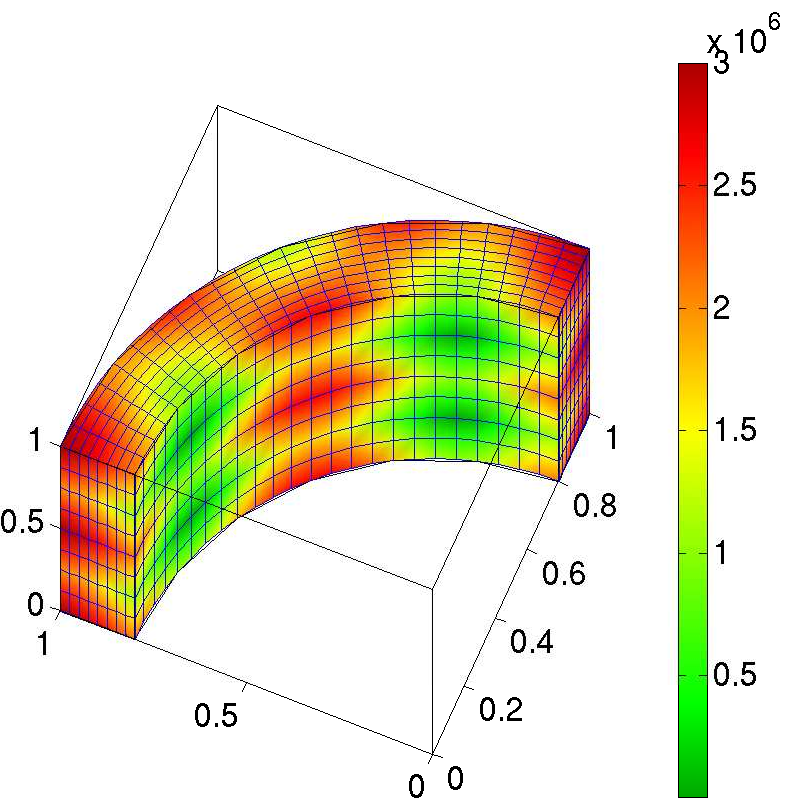
\includegraphics[width=0.48\textwidth]{figs/fan3a}
	\caption{\label{fig:mesh} Two and three dimensional warped
          meshes used in our numerical experiments. The color
          illustrates the value of the coefficient $\mu(\bs x)$.}
\end{figure}


\subsection{Setup of comparisons}\label{subsec:measures}
Tables \ref{tab:box}--\ref{tab:3d-fan} present the number of multigrid
v-cycles or of conjugate gradient (CG) iterations required to reduce
the norm of the discrete residual by a factor of $10^8$. In
particular, these tables report the following.
\begin{itemize}
\item[$\bullet$] The first column gives the polynomial \emph{order}
  used in the finite element discretization.
\item[$\bullet$] The columns entitled by \emph{MG as solver} report
  the number of v-cycles needed when multigrid is used as a
  solver. The subcolums are:
  \begin{itemize}
  \item \emph{Jacobi(3,3)} denotes that 3 pre-smoothing and 3
    post-smoothing steps of a pointwise Jacobi smoother are used on
    each level.
  \item \emph{Cheb(3,3)} indicates that Chebyshev-accelerated Jacobi
    smoothing is used, again with 3 pre-smoothing and 3
    post-smoothing steps. The maximal eigenvalue required by the
    Chebyshev method is estimated using \todo{XX iterations of
      Lanczos}.
  \item \emph{SSOR(2,1)} denotes that a symmetric successive
    over-relaxation method is employed, where 2 pre-smoothing and 1
    post-smoothing step are employed. Note that each SSOR smoothing
    iteration amounts to a forward and a backward v-cycle, and thus
    requires double the computational work compared to Jacobi
    smoothing.\footnote{This ignores aspects occurring in parallel
      environments, where Gauss-Seidel smoothing---such as SSOR---can
      be challenging to implement and requires more communication in
      distributed memory environments.}. The SSOR smoother is based on 
			a lexicographic ordering of  the unknowns. 
  \end{itemize}
  Note that for each smoother we report results for
  $h$-multigrid (columns marked by \emph{h}; see
  \S\ref{subsec:h}) as well as for $p$-multigrid (columns marked
  by \emph{p}; see \S\ref{subsec:p}). For $p$-multigrid, we
  restrict ourselves to orders that are powers of 2. After
  coarsening in $p$ till $p=1$, we coarsen in $h$. \todo{how
    many levels? what size meshes?}
\item[$\bullet$] The columns entitled \emph{MG with pCG} presents our
  results obtained when multigrid is uses as preconditioner in a CG
  algorithm. The sub-columns again correspond to different smoothers,
  as described above.
\item[$\bullet$] The columns headed by \emph{linearized pCG} present
  the number of CG iterations needed to solve the high-order system
  preconditioned with the low-order operator based on the high-order
  node points (see \S\ref{subsec:low}). While in practice one
  would most likely use an algebraic multigrid cycle to approximately
  solve the linearized system, here we use a direct factorization
  method as solver for the low-order system. The different columns
  correspond to different numbers of Chebyshev-accelerated Jacobi
  smoothing steps on the finest mesh. These smoothing steps use the
  high-order residual but the diagonal from the low-order system. As a
  consequence, the Chebyshev smoother requires an estimate of the
  largest eigenvalue of the high-order matrix preconditioned with the
  diagonal of the low-order operator, which is computed using
  \todo{XX} steps of the Lanzos algorithm.
\end{itemize}
In the next section, we summarize our numerical comparisons.

\subsection{Summary of numerical results}\label{subsec:results}
The Tables \ref{tab:box} and \ref{tab:2d-fan} present our results for
the two dimensional test problems. As can be seen in
Table~\ref{tab:box}, for the Laplace problem on the unit square all
solver/smoothing variants converge for all polynomial orders in a
relatively small number of iterations. However, the number of
iterations increases with the polynomial orders $p$, in particular
when multigrid is used as a solver. Using multigrid as a
preconditioner in CG results in a reduction of multigrid v-cycles, in
some cases even by a factor or two. Also, we observe that SSOR
smoothing generally performs better than the two Jacobi-based
smoothers. We find that the linear-order operator based on the
high-order nodes is a good preconditioner for the high-order
system. The convergence of this method is significantly improved when
smoothing steps on the finest level are used. Note that the Jacobi
smoother underlying the Chebyshev smoother uses the diagonal entries
of the low-order operator, but the residual computed from the
high-order operator. The low-order preconditioning approach proves to
be efficient, making it particularly attractive for high-order
discretized problems on unstructured meshes. However, in our tests
this efficiency partly has to be attributed to the use of a direct
solver for the low-order system, rather than an approximate solution
based on an algebraic multigrid method.

% \gsnote{It's interesting that with 3 smoothing steps this
%  performs better than the high-order multigrid with Chebyshev
%  smoother---the computational work is comparable; but I think this
%  might be caused by the direct solves on the coarse level.}

\begin{table}
  \caption{\label{tab:box} Results for two-dimensional unit square
    with constant coefficient $\mu\equiv 1$.  A total of 3 grids were
    used, the finest grid was $32\times 32$, and the coarsest was
    $8\times 8$. For a detailed description of the different
    experiments reported in this table we refer to
    \S\ref{subsec:measures}.}  \centering
  \begin{tabular}{|r|c c|c c|c c||c c|c c|c c||c c c|} 
    \hline
    & \multicolumn{6}{c||}{MG as solver} & \multicolumn{6}{c||}{MG with pCG} & \multicolumn{3}{r|}{linearized} \\
    \cline{2-13}
    \!\!\! order \!\!\!\! &  \multicolumn{2}{c|}{\!\scriptsize  Jacobi(3)\!} &  \multicolumn{2}{c|}{\!\scriptsize Cheb(3)\!} & \multicolumn{2}{c||}{\!\scriptsize  SSOR(2)\!} & \multicolumn{2}{c|}{\!\scriptsize Jacobi(3)\!} &  \multicolumn{2}{c|}{\!\scriptsize Cheb(3)\!} & \multicolumn{2}{c||}{\!\scriptsize SSOR(2)\!} & \multicolumn{3}{c|}{pCG}\\
\hline
 & $h$ & $p$ & $h$ & $p$& $h$ & $p$& $h$ & $p$& $h$ & $p$& $h$ & $p$& 0 & 1 & 3\\
 \cline{2-16}
1 & 6 & & 5 & & 5 & & 5 & & 4 & & 4 & & - & - & - \\
2 & 7 & 7 & 5 & 6 & 5 & 5 & 5 & 5 & 4 & 4 & 4 & 4 & 14 & 9 & 4 \\
3 & 8 & & 6 & & 5 & & 6 & & 5 & & 4 & & 16 & 9 & 4 \\
4 & 9 & 8 & 6 & 6 & 5 & 5 & 6 & 5 & 5 & 5 & 4 & 4 & 16 & 10 & 4 \\
5 & 12 & & 8 & & 7 & & 7 & & 6 & & 5 & & 17 & 10 & 4 \\
6 & 12 & & 9 & & 7 & & 7 & & 6 & & 5 & & 18 & 11 & 5\\
7 & 16 & & 12 & & 8 & & 8 & & 7 & & 6 & & 18 & 12 & 5 \\
8 & 17 & 14 & 13 & 10 & 8 & 7 & 9 & 8 & 7 & 6 & 6 & 5 & 19 & 12 & 5\\
16 & 40 & 33 & 33 & 27 & 17 & 14 & 14 & 12 & 12 & 11 & 9 & 8 & 21 & 14 & 8 \\
\hline
  \end{tabular}
\end{table}


Let us now contrast these observations with the results for the
variable coefficient case summarized in Table~\ref{tab:2d-fan}. First,
note that all variants perform reasonably for discretizations up to
order $p=4$. When used as a solver, multigrid either diverges or
converges very slowly for orders $p>4$. Convergence is reestablished
when multigrid is combined with CG.

Next, we turn to the three dimensional results reported in
Tables~\ref{tab:3d-box} and \ref{tab:3d-fan}. All of our
multigrid/smoother variants converge for the Laplace equation on the
unit cube, as shown in Table~\ref{tab:3d-box}. The benefit of using
multigrid as preconditioner rather than as solver is even more evident
in three dimensions than for the two dimensional unit square
problem. \todo{Need to comment on linearized preconditioner.}

Our results for varying coefficient problem on the three-dimensional
geometry shown in Figure~\ref{fig:mesh} are summarized in
Table~\ref{tab:3d-fan}. As in two dimensions, the performance of
multigrid when used as a solver degrades significantly for orders
$p>4$.


\begin{table}
  \caption{\label{tab:2d-fan} Results for two-dimensional warped
    geometry with varying coefficient $\mu(x,y) = 1 + 10^6(\cos^2(2\pi
    x) + \cos^2(2\pi y))$.  A total of 3 grids were used, the finest
    grid was $32\times 32$, and the coarsest was $8\times 8$. For a
    detailed description of the different experiments reported in this
    table we refer to \S\ref{subsec:measures}.}  \centering
  \begin{tabular}{|r|c c|c c|c c||c c|c c|c c||c c c|} 
    \hline
    & \multicolumn{6}{c||}{MG as solver} & \multicolumn{6}{c||}{MG with pCG} & \multicolumn{3}{r|}{linearized} \\
    \cline{2-13}
    \!\!\! order \!\!\!\! &  \multicolumn{2}{c|}{\!\scriptsize  Jacobi(3)\!} &  \multicolumn{2}{c|}{\!\scriptsize Cheb(3)\!} & \multicolumn{2}{c||}{\!\scriptsize  SSOR(2)\!} & \multicolumn{2}{c|}{\!\scriptsize Jacobi(3)\!} &  \multicolumn{2}{c|}{\!\scriptsize Cheb(3)\!} & \multicolumn{2}{c||}{\!\scriptsize SSOR(2)\!} & \multicolumn{3}{c|}{pCG}\\
\hline
 & $h$ & $p$ & $h$ & $p$& $h$ & $p$& $h$ & $p$& $h$ & $p$& $h$ & $p$& 0 & 1 & 3\\
 \cline{2-16}
1 & 14 & & 11 & & 6 & & 8 & & 7 & & 5 & & - & - & - \\
2 & 20 & 19 & 15 & 15 & 7 & 8 & 10 & 10 & 8 & 8 & 5 & 6 & 16 & 9 & 5 \\
3 & 20 & & 16 & & 8 & & 10 & & 9 & & 6 & & 18 & 9 & 6 \\
4 & 22 & 21 & 21 & 19 & 10 & 9 & 11 & 10 & 10 & 10 & 7 & 6 & 19 & 11 & 7\\
5 & -  & & 28 & & 12 & & 14 & & 12 & & 7 & & 21 & 12 & 8  \\
6 & -  & & 35 & & 13 & & 15 & & 13 & & 8 & & 23 & 13 & 9 \\
7 & -  & & 45 & & 16 & & 18 & & 15 & & 9 & & 24 & 14 & 9 \\
8 & -  & - & 52 & 46 & 17 & 15 & 20 & 20 & 16 & 15 & 9 & 8 & 25 & 14 & 10 \\
16 & - & - & 169 & 148 & 37 & 33 & 51 & 45 & 30 & 27 & 13 & 12 & 31 & 19 & 13 \\
\hline
  \end{tabular}
\end{table}


\begin{table}
  \caption{\label{tab:3d-box} Results for three-dimensional cube
    geometry with constant coefficient $\mu(\bs x) \equiv 1$. For a
    detailed description of the different experiments reported in this
    table we refer to \S\ref{subsec:measures}.}  \centering
	  \begin{tabular}{|r|c c|c c|c c||c c|c c|c c||c c c|} 
	    \hline
	    & \multicolumn{6}{c||}{MG as solver} & \multicolumn{6}{c||}{MG with pCG} & \multicolumn{3}{r|}{linearized} \\
	    \cline{2-13}
	    \!\!\! order \!\!\!\! &  \multicolumn{2}{c|}{\!\scriptsize  Jacobi(3)\!} &  \multicolumn{2}{c|}{\!\scriptsize Cheb(3)\!} & \multicolumn{2}{c||}{\!\scriptsize  SSOR(2)\!} & \multicolumn{2}{c|}{\!\scriptsize Jacobi(3)\!} &  \multicolumn{2}{c|}{\!\scriptsize Cheb(3)\!} & \multicolumn{2}{c||}{\!\scriptsize SSOR(2)\!} & \multicolumn{3}{c|}{pCG}\\
	\hline
	 & $h$ & $p$ & $h$ & $p$& $h$ & $p$& $h$ & $p$& $h$ & $p$& $h$ & $p$& 0 & 1 & 3\\
	 \cline{2-16}
1 & 6 & & 4 & & 4 & & 5 & & 4 & & 3 & & - & - & - \\
2 & 8 & 8 & 4 & 5 & 4 & 5 & 6 & 6 & 4 & 4 & 4 & 4 &  25 & 14 & 5 \\
3 & 10 & & 7 & & 5 & & 6 & & 5 & & 5 & & 27 & 13 & 5  \\
4 & 11 & 10 & 8 & 7 & 6 & 5 & 7 & 7 & 6 & 5 & 5 & 4 & 28 & 15 & 6 \\
5 & 14 & & 10 & & 7 & & 8 & & 7 & & 5 & & 29 & 16 & 6 \\
6 & 16 & & 11 & & 7 & & 9 & & 7 & & 6 & & 32 & 18 & 6 \\
7 & 20 & & 15 & & 9 & & 10 & & 9 & & 6 & & 34 & 19 & 7 \\
8 & 22 & 19 & 17 & 15 & 9 & 8 & 10 & 10 & 9 & 8 & 6 & 6 & 35 & 20 & 7 \\
16 & 47 & 42 & 38 & 34 & 17 & 15 & 16 & 14 & 14 & 13 & 9 & 9 & 39 & 22 & 11 \\
\hline 
 \end{tabular}
\end{table}

\begin{table}
  \caption{\label{tab:3d-fan} Results for three-dimensional warped
    geometry with varying coefficient $\mu(x,y,z) = 1 +
    10^6(\cos^2(2\pi x) + \cos^2(2\pi y) + \cos^2(2\pi z))$. For a
    detailed description of the different experiments reported in this
    table we refer to \S\ref{subsec:measures}.}  \centering
	  \begin{tabular}{|r|c c|c c|c c||c c|c c|c c||c c c|} 
	    \hline
	    & \multicolumn{6}{c||}{MG as solver} & \multicolumn{6}{c||}{MG with pCG} & \multicolumn{3}{r|}{linearized} \\
	    \cline{2-13}
	    \!\!\! order \!\!\!\! &  \multicolumn{2}{c|}{\!\scriptsize  Jacobi(3)\!} &  \multicolumn{2}{c|}{\!\scriptsize Cheb(3)\!} & \multicolumn{2}{c||}{\!\scriptsize  SSOR(2)\!} & \multicolumn{2}{c|}{\!\scriptsize Jacobi(3)\!} &  \multicolumn{2}{c|}{\!\scriptsize Cheb(3)\!} & \multicolumn{2}{c||}{\!\scriptsize SSOR(2)\!} & \multicolumn{3}{c|}{pCG}\\
	\hline
	 & $h$ & $p$ & $h$ & $p$& $h$ & $p$& $h$ & $p$& $h$ & $p$& $h$ & $p$& 0 & 1 & 3\\
	 \cline{2-16}
1 & 13 & & 7 & & 5 & & 7 & & 5 & & 4 & & - & - & - \\
2 & 17 & 18 & 13 & 13 & 7 & 7 & 9 & 9 & 8 & 8 & 5 & 5 & 26 & 14 & 7 \\
3 & 20 & & 16 & & 8 & & 10 & & 9 & & 6 & & 29 & 14 & 8 \\
4 & 23 & 22 & 18 & 18 & 9 & 9 & 11 & 11 & 9 & 9 & 7 & 6 & 31 & 16 & 9\\
5 & 26 & & 21 & & 10 & & 12 & & 10 & & 7 & & 34 & 17 & 10  \\
6 & 30 & & 27 & & 12 & & 13 & & 12 & & 8 & & 37 & 20 & 13 \\
7 & 35 & & 34 & & 14 & & 14 & & 14 & & 8 & & 37 & 21 & 13  \\
8 & - & - & 40 & 38 & 16 & 15 & 18 & 17 & 15 & 14 & 9 & 9 & 38 & 21 & 14 \\
16 & - & - & 117 & 110 & 32 & 29 & 67 & 60 & 27 & 26 & 13 & 13 & 47 & 28 & 22 \\
\hline
  \end{tabular}
\end{table}

In the next section, we summarize our findings and draw conclusions.

\section{Discussion and conclusions}
\label{sec:discuss}

Despite the fact that discrete systems originating from high-order
discretizations do not satisfy favorable matrix properties such as the
M-matrix property, we find that point smoothers can be efficient for
polynomial orders up to $p=16$.  For constant coefficient, two and
three-dimensional problems, all tested point smoothers (Jacobi,
Chebyshev-accelerated Jacobi and Gauss-Seidel SSOR smoothing) lead to
converging multigrid methods. For highly varying coefficients on
deformed geometries, SSOR outperforms Jacobi-based smoothing, which
performs poorly for orders $p>4$.

In a parallel environment, where Gauss-Seidel smoothing is
significantly more difficult to implement and requires more parallel
communication, Chebyshev-accelerated Jacobi smoothing represents an
interesting alternative since it is as simple to implement as Jacobi
smoothing.

Using multigrid as preconditioner in a Krylov method rather than as
solver results in significantly faster convergence, which by far
compensates for the additional work required by the Krylov method,
namely vector additions and inner products.  For problems with varying
coefficients, we found that the number of required v-cycles decreases
by up to a factor of three when combining multigrid with the conjugate
gradient method.

We find that a low order operator based on the high-order node points
is an excellent preconditioner for the low-order system, in particular
when combined with smoothing based on the high-order residual is
performed on the finest mesh.  When combined with algebraic multigrid
for the low-order operator, this approach is attractive for high-order
discretizations on unstructured meshes as also shown in
~\cite{Brown10, DevilleMund90, HeysManteuffelMcCormickEtAl05}.


%low-order preconditioner competitive w.r. to number of
%  iterations; thus a good option as preconditioner when using AMG for
%  unstructured high-order meshes

\section*{Acknowledgments}
We would like to thank Tobin Isaac for helpful discussions on the
low-order preconditioner. Support for this work was
  provided through the U.S.~National Science Foundation (NSF) grants
  CMMI-1028889 and   % CDI mantle/wave
  ARC-0941678,       % NSF ice
 and through the Scientific Discovery through Advanced
  Computing (SciDAC) projects 
  DE-SC0009286,   % Diamond
%  DE-SC0006656,  % Quest
  and DE-SC0002710 % UQ ice
  funded by the U.S.~Department of Energy
  Office of Science, Advanced Scientific Computing Research and
  Biological and Environmental Research.
 \todo{Check with George and Omar; these are Diamond, DOE ice, NSF ice and NSF mantle/wave.}


\bibliographystyle{siam}
\bibliography{ccgo}


\end{document}
